\documentclass{article}

\usepackage[utf8]{inputenc}
\usepackage[francais]{babel}
\usepackage{geometry}
\usepackage{graphicx}
\usepackage{amsfonts}
%\usepackage{pgfgantt}
\usepackage{tikz}

\title{Projet base de données\\
------ \\
\large{Traitement des emplois du temps du département informatique}\\
\small{Enseignant responsable : Claude Sabatier}}
\author{Lionel Dromer \and \'Eloi Perdereau}
\date{\today}

\sloppy
\geometry{dvips,a4paper,margin=1in}

\begin{document}

\maketitle
\tableofcontents
\newpage

\section{Cahier des charges}

\subsection{\'Etude de l'existant}
Nous ne pouvons avoir qu'un point de vue de l'utilisateur final, mais en étudiant différents modèles d'emploi du temps, nous avons pu relever des fonctionnalités récurrentes, avec des subtilités :
\begin{itemize}
\item Deux sens possibles d'affichage des jours : vertical ou horizontal.
\item Afficher l'emploi du temps de promotions, d'enseignants ou de salles. Possibilité de les combiner.
\item Choisir la période.
\item Différents formats d'exportation (PDF, impression, ...).
\item Modification de l'emploi du temps par un administrateur.
\item Couleurs par UE\footnote{UE = Union d'Enseignements}.
\item Libelle d'un créneau adapté selon l'affichage.
\item Version mobile disponible.
\end{itemize}

En voici deux exemples :

\begin{figure}[!ht]
\begin{center}
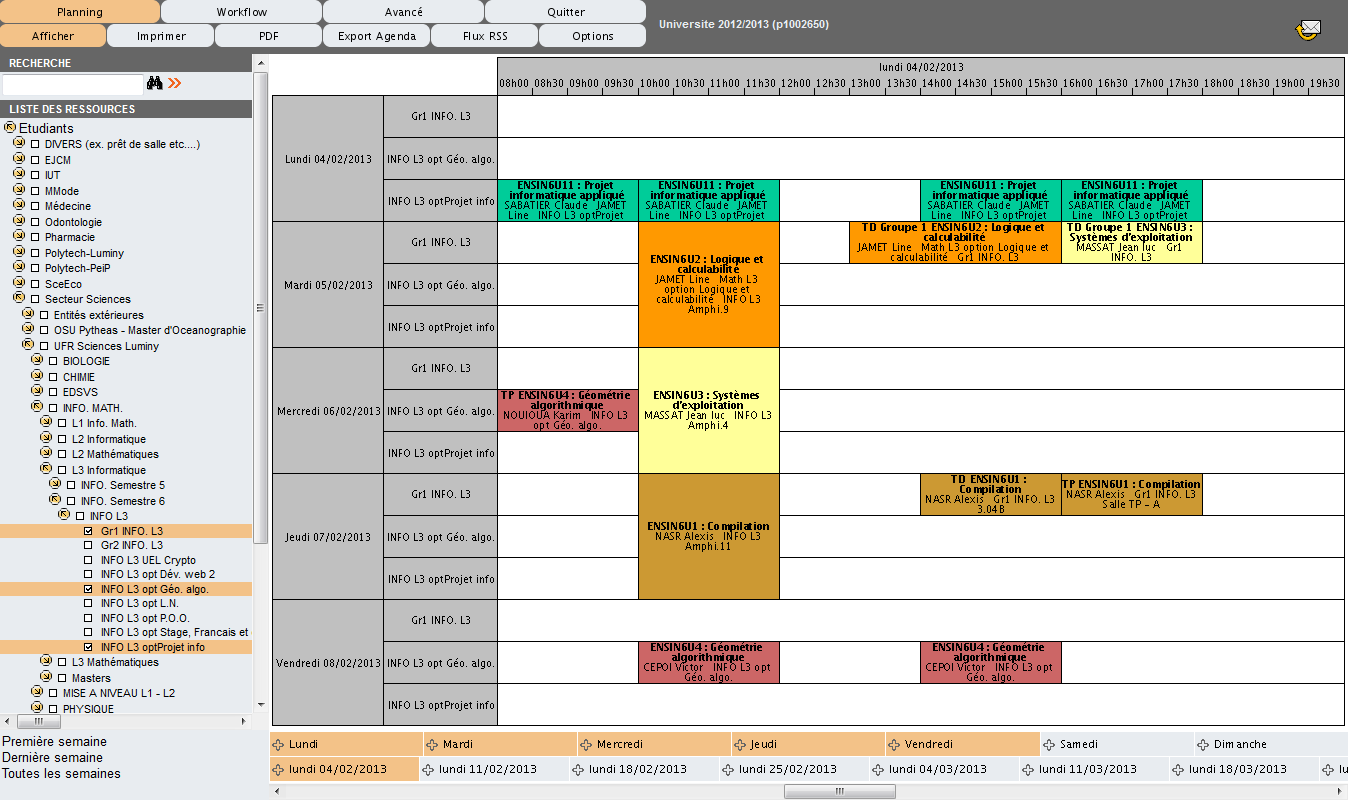
\includegraphics[scale=0.5]{img/edt_ade.png}
\caption{ADE : Emploi du temps de l'AMU}
\end{center}
\end{figure}

\newpage
\begin{figure}[!ht]
\begin{center}
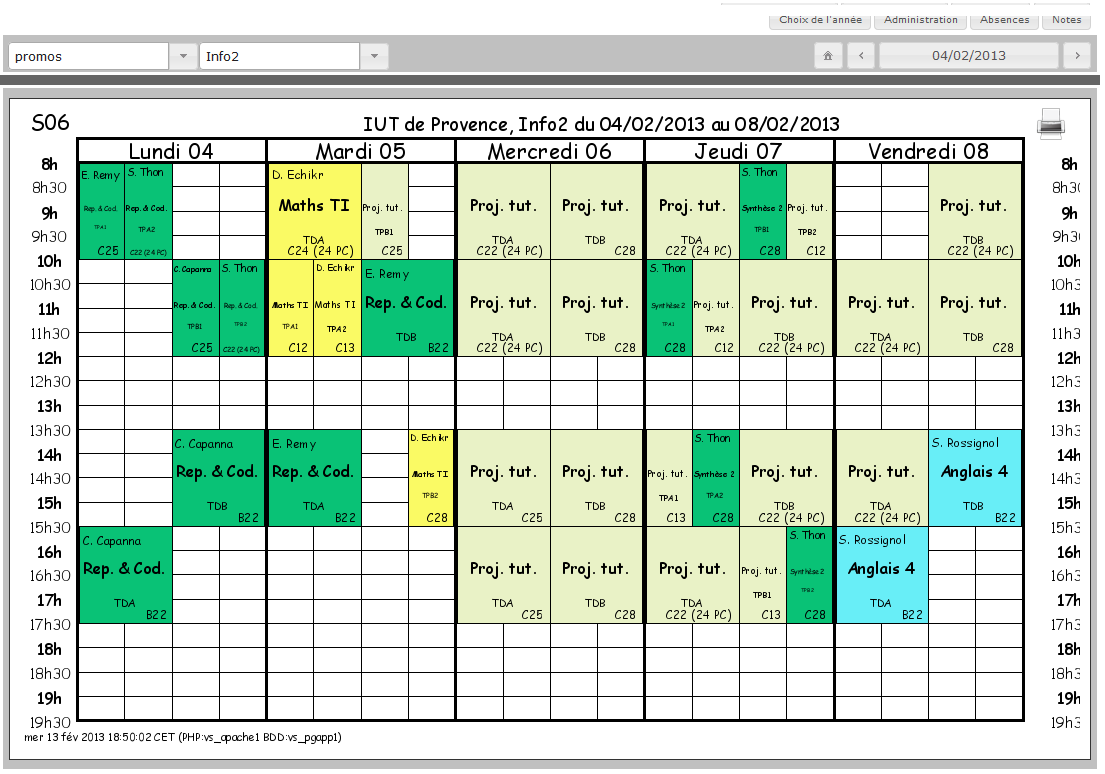
\includegraphics[scale=0.6]{img/edt_iut_arles.png}
\caption{Emploi du temps de l'IUT d'Arles}
\end{center}
\end{figure}



\subsection{\'Etude des besoins}
Afin de répondre à la problématique posée, on a pu relever les fonctionnalités suivantes :
\begin{itemize}
\item Vérifier la cohérence de toutes les horaires, au niveau des enseignants, des étudiants et des salles.
\item Modification de l'emploi du temps : déplacer une séance. Vérifier la disponibilité des participants (étudiants, enseignant, salle) avant de l'enregistrer.
\item Placement des séances selon un programme pédagogique donné.
\item \'Editer des récapitulatifs lisibles (couleurs et libellés adaptés) :
    \begin{itemize}
    \item Emploi du temps d'une promotion donnée (tout groupes de TD confondus ou d'un groupe donné), pour une période donnée.
    \item Emploi du temps d'un enseignant donné, pour une période donnée.
    \item Occupation d'une salle donnée pour une période donnée.
    \item Nombre total d'heures d'enseignement reçues par un étudiant d'une promotion donnée.
    \item Nombre d'heures de Cours, TD et TP assurés par un enseignant donné (et les équivalents TD correspondant) pour toutes les UE et toutes les promotions.
    \end{itemize}
\end{itemize}

\subsection{\'Etude de faisabilité (outils)}
Technologies à notre disposition :
\begin{itemize}
\item Langage Java
\item JPA ou JDBC + DAO
\item SGBD Oracle
\end{itemize}

Gestion de projet :
\begin{itemize}
\item Maven
\item Gestionnaire de version Git
\item Gestion de projet Gantt
\item \'Equipe de deux développeurs
\end{itemize}

\begin{figure}[!h]
\begin{center}
%\begin{ganttchart}[y unit title=0.4cm,
%y unit chart=0.5cm,
%vgrid,hgrid,
%title label anchor/.style={below=-1.6ex},
%title height=1,
%bar/.style={fill=gray!50},
%bar height=0.7,]{24}
%%labels
%\gantttitle{Février}{6}
%\gantttitle{Mars}{6}
%\gantttitle{Avril}{6}
%\gantttitle{Mai}{6} \\
%%tasks
%\ganttbar{Cahier des charges}{1}{3} \\
%\ganttbar{MCD}{4}{8} \\
%\ganttbar{MCT}{4}{7} \\
%\ganttbar{Interface graphique}{8}{18} \\
%\ganttbar{Modèle}{9}{20} \\
%\ganttbar{Tests}{14}{22} \\
%\ganttbar{Rapport}{21}{24}
%%relations
%\ganttlink{elem0}{elem1}
%\ganttlink{elem0}{elem2}
%\ganttlink{elem1}{elem4}
%\ganttlink{elem2}{elem3}
%\ganttlink{elem3}{elem6}
%\ganttlink{elem4}{elem6}
%\end{ganttchart}
\end{center}
\caption{Diagramme de Gantt}
\end{figure}

\subsection{Analyse préalable}

\subsubsection{Scénarios}
La structure pédagogique est fixe. Cela veux dire que les UE et leurs spécificités sont déjà présentes dans la base. Aucune interface n'est prévu pour modifier ces données. C'est à dire que seul un accès direct à la base de donnée permet la modification de la structure pédagogique.

\paragraph{Du point de vue de l'utilisateur final :\\}
Il y a deux types d'utilisateurs finaux : les enseignants et le public.
Le public ne peut que consulter l'emploi tu temps.
Les enseignants, ont également le droit de consulter l'état de leur service. Certains enseignants peuvent être gestionnaire (cf. paragraphe suivant).
Lorsqu'un utilisateur veut consulter l'emploi du temps, il doit d'abord dérouler un arbre dans lequel il sélectionne les différentes UE à afficher. Par salle, par année et groupe ou par enseignant.

\paragraph{Du point de vue des gestionnaires de l'emploi du temps :\\}
Il y a plusieurs gestionnaires de l'emploi du temps ; ils travailleront de manière concurrente. On distingue en distingue deux types avec des droits spécifiques :
\begin{itemize}
\item Le gestionnaire d'année : il peut placer les séances auquel participerons les étudiants de l'année (des années) dont le gestionnaire à les droits.
\item Le gestionnaire des professeurs : il peut modifier le nombre d'heures de services effectués par tous les enseignants, ainsi que leur ajouter une période d'indisponibilité.
\end{itemize}

Un gestionnaire peut faire les mêmes actions qu'un utilisateur classique. Lorsqu'il veut effectuer des tâches administratives, il doit se connecter via un bouton. Dès lors, une zone contenant différents boutons se présente à lui. Ces boutons affichent des panneaux dans lesquels le gestionnaire peut effectuer des tâches administratives.

\begin{itemize}
\item Pour un gestionnaire d'année(s) :
La zone contient un bouton par année gérée. Chacun affiche un panneau contenant les cours/TD/TP/heures de projet restant à placer (pour l'année en question), avec le nombre d'heures associés. Le panneau contient également des champs à remplir pour placer une séance (date de début, durée). Lorsqu'il veux placer un cours, il sélectionne le cours en question dans le panneau. Une fois le cours sélectionné et les champs remplis, un bouton valider calcule si tous les participants sont disponibles (étudiants, enseignants, salle). Si oui, une salle est attribuée automatiquement et une boîte de dialogue s'affiche permettant au gestionnaire de choisir le professeur à affecter. Ensuite le créneau est placé dans l'emploi du temps. Si les étudiants ne sont pas disponibles où qu'aucune salle n'est libre, un message d'erreur averti le gestionnaire avec le motif de refus. Les champs précédemment remplis pourront être modifiés en conséquence.
Un créneau est compris entre 8 heures et 20 heures du lundi au vendredi.\\

\item Pour un gestionnaire d'enseignant :
Le panneau se divise en deux avec une liste déroulante contenant la liste des enseignants en en-tête.
Une partie lui montre un formulaire pour ajouter une période d'indisponibilité. Cet ajout peut être refusé si l'enseignant en question a déjà un cours de prévu dans le créneau indiqué.
L'autre partie lui permet de modifier le nombre d'heures d'administrations effectués.
\end{itemize}

Un gestionnaire peut être à la fois gestionnaire de plusieurs années et gestionnaire d'enseignant en même temps.

\subsubsection{Cas particuliers}
\begin{itemize}
\item Avertissement lorsqu'une séance est placée dans un créneau peu commode (pause déjeuner, après 18 heures, etc...).
\item Avertissement lorsqu'une séance est placée moins de 48 heures avant sa date de début.
\item Avertissement si le nombre d'heures de TD, TP ou Projet est différent pour différents groupes d'une même promotion.
\end{itemize}

\section{Analyse détaillée}

\subsection{\'Etude des données}

\subsubsection{Dictionnaire des données}

\hspace*{-0.6in}
\begin{tabular}{|p{4cm}|p{8cm}|p{5cm}|}
  \hline
  Nom attribut & Description & Contrainte(s) \\
  \hline

  IdNiveau & Id du niveau d'une promotion (son année) & unique \\

  LibelleNiveau & Libellé du niveau d'une promotion (e.g : 'L1', 'M2') & $\emptyset$ \\

  IdUE & Identifiant d'une UE & unique \\

  LibelleUE & Libelle d'une UE & unique \\

  NbHeuresCours & Nombre d'heures de cours concernant une UE & $> 0$ \\

  NbHeuresTD & Nombre d'heures de TD concernant une UE & $> 0$ \\

  NbHeuresTP & Nombre d'heures de TP concernant une UE & $> 0$ \\

  NbHeuresProjet & Nombre d'heures de Projet concernant une UE & $\geq 0$ \\

%  NbHeuresCoursPlacees & Nombre d'heures de cours placées concernant une UE & $\geq 0\ ;\ \leq$ NbHeuresCours \\

%  NbHeuresTDPlacees & Nombre d'heures de TD placées concernant une UE & $\geq 0\ ;\ \leq$ NbHeuresTD \\

%  NbHeuresTPPlacees & Nombre d'heures de TP placées concernant une UE & $\geq 0\ ;\ \leq$ NbHeuresTP \\

%  NbHeuresProjetPlacees & Nombre d'heures de Projet placées concernant une UE & $\geq 0\ ;\ \leq$ NbHeuresProjet \\

  IdPromo & Identifiant d'une promotion & unique \\

  EffectifPromo & Effectif d'une promotion & $> 0$ \\

  IdGroupe & Identifiant d'un groupe de TD & unique \\

  EffectifGroupe & Effectif d'un groupe & $> 0$ \\

  NomEns & Nom d'un enseignant & $\emptyset$ \\

  RattachementEns & Site de rattachement d'une enseignant & $\in$ \{'Departement informatique', 'Exterieur'\} \\

%  GradeEns & Grade d'un enseignant & $\in$ \{'Maitre de conferences', 'Professeur', 'PRAG', 'PAST', 'ATER', 'Moniteur'\} \\

  NoTelEns & Numéro de téléphone correspondant du bureau qu'un enseignant occupe & $\emptyset$ \\

  MailEns & Adresse e-mail d'un enseignant & $\emptyset$ \\

  NbHeuresAdminEns & Nombre d'heures qu'un enseignant a effectué & $> 0$ \\

  IdGrade & Identifiant d'un grade d'un enseignant & unique \\

  LibelleGrade & Libelle d'un grade d'un enseignant & $\emptyset$ \\

  DateDebutIndisponibilite & Date de début d'une période d'indisponibilité pour un enseignant & $\emptyset$ \\

  DureeIndisponibilite & Durée d'une période d'indisponibilité pour un enseignant & $> 0$ \\

  IdSalle & Identifiant d'une salle & unique \\

  NoSalle & Numéro d'une salle & $\emptyset$ \\

  EffectifMax & Effectif maximal d'une salle & $> 0$ \\

  IdTypeSalle & Identifiant d'un type de salle & unique \\

  LibelleTypeSalle & Libelle d'un type de salle (e.g : 'Amphi', 'TD', 'TP'). & $\emptyset$ \\

  IdTypeSeance & Identifiant du type de séance\footnote{séance : Cours, TD, TP ou Projet en train de se dérouler} & unique \\

  LibelleTypeSeance & Libelle du type de séance (e.g : 'Cours', 'TD', 'TP', 'Projet') & $\emptyset$ \\

  CoefEquivalentTD & Coefficient d'équivalent TD d'un type de séance & $> 0$ \\

  DateDebutSeance & Date de début d'une séance & $\emptyset$ \\

  DureeSeance & Durée d'une séance & $> 0\ ;\ \leq 4$ \\

  IdGest & Identifiant numérique d'un gestionnaire & unique \\

  LoginGest & Identifiant servant à un gestionnaire d'emploi du temps pour se connecter & $\emptyset$ \\

  PwGest & Mot de passe servant à un gestionnaire d'emploi du temps pour se connecter & $\emptyset$ \\

  IsGestEns & Indique si l'utilisateur est un gestionnaire d'enseignant ou non & $\emptyset$ \\

  \hline
\end{tabular}

\newpage

\subsubsection{Modèle Conceptuel des Données}
\begin{figure}[!ht]
\hspace*{-0.9in}
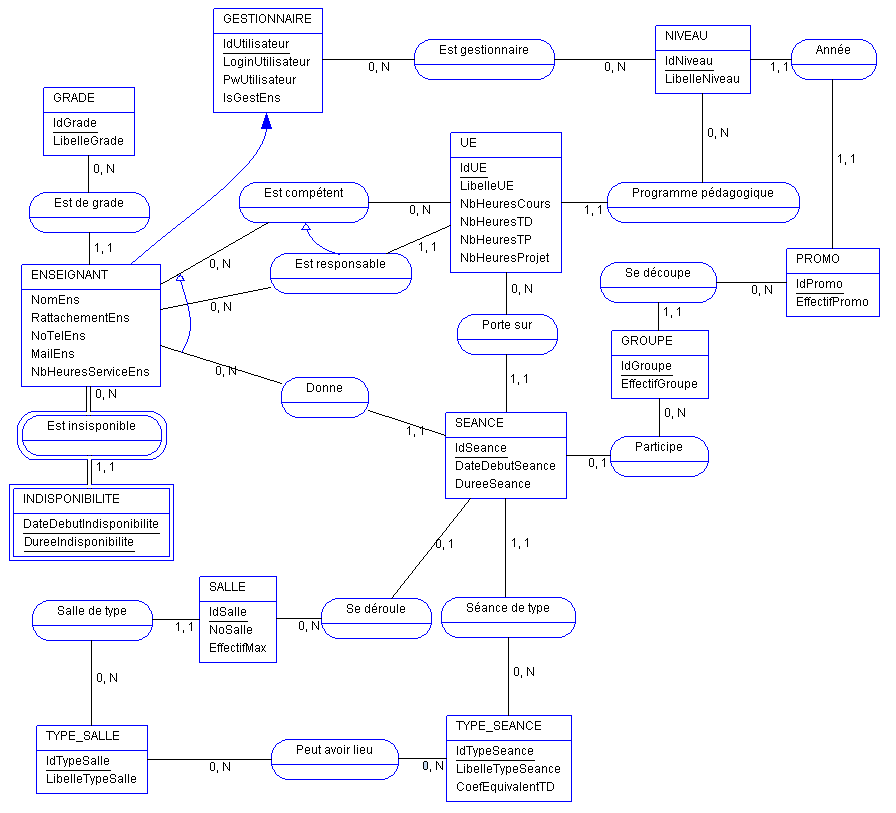
\includegraphics[scale=0.9]{img/MCD.png}
\caption{MCD}
\end{figure}

On conviendra que si aucun groupe ne participe à une séance, alors c'est toute la promotion du niveau de l'UE qui y participe.

\subsubsection{Contraintes}

\begin{itemize}
\item Un enseignant ne peut participer à une séance uniquement s'il ne participe pas déjà à une séance dont la période chevauche celle de la séance en question. De plus, il ne doit pas être indisponible durant la période de la séance.

\item Une promotion ne peut participer à une séance uniquement si elle ne participe pas déjà à séance dont la période chevauche celle de la séance en question. Idem pour un groupe.

\item Une salle ne peut être affecté à une séance uniquement si elle n'est pas déjà affecté à une séance dont la période chevauche celle de la séance en question.

\item Une séance ne peut avoir lieu uniquement dans une salle qui a un effectif plus faible que l'effectif du groupe ou de la promotion qui participe à la séance.

\item Une séance ne peut avoir lieu uniquement dans une salle dont le type est compatible à celui de la séance.

\item Une séance ne peut pas durer plus de 4 heures.

\item La somme des durées des séances pour une UE donnée et un type de séance donné ne doit pas dépasser le nombre d'heures prévu pour cette UE pour ce type de séance.

\item Aucune séance ne doit avoir lieu avant 8 heures ou après 20 heures.

\item La date de début d'une séance ajoutée ou modifiée doit être postérieur au présent. Idem pour la date de début d'une indisponibilité.

\item L'effectif de l'ensemble des groupes d'une promotion doit être égal à l'effectif de la promotion concernée.

\item Une promotion (ou un groupe) ne peut participer uniquement à des séances de son niveau.

\item Un groupe ne peut pas participer à une séance de type 'Cours'.

\item Une période d'indisponibilité ne peut être ajoutée (ou modifiée) si l'enseignant concerné participe à une séance chevauchant la période sus-dite.

\item Si un individu est connecté et qu'il n'est pas gestionnaire, c'est un enseignant. En effet, seulement trois types d'individus pourront se connecter : les enseignants, les gestionnaires d'années et les gestionnaires d'enseignants. Malheureusement, cette contrainte ne pourra pas être vérifiée en base. Prenons un exemple : nous voulons ajouter un nouveau gestionnaire d'année. Il faut d'abord insérer le gestionnaire en question avec ses identifiants, puis insérer le (premier) lien qui le lie à une année. Entre ces deux insertions, la contrainte ne sera pas satisfaite. Néanmoins, nous pouvons empêcher un individu de se connecter s'il n'est ni gestionnaire ni enseignant.

\end{itemize}

\subsection{\'Etude des fonctionnalités de l'application}

\subsubsection{Scénarios}

\subsubsection{Modèle Conceptuel des Traitements}
\begin{figure}[!ht]
\advance\leftskip-1.9in
% Graphic for TeX using PGF
% Title: /filer/etudiants/g7/p1002650/Bureau/dias/MCT1.dia
% Creator: Dia v0.97.1
% CreationDate: Fri Apr  5 16:00:33 2013
% For: p1002650
% \usepackage{tikz}
% The following commands are not supported in PSTricks at present
% We define them conditionally, so when they are implemented,
% this pgf file will use them.
\ifx\du\undefined
  \newlength{\du}
\fi
\setlength{\du}{15\unitlength}
\begin{tikzpicture}
\pgftransformxscale{1.000000}
\pgftransformyscale{-1.000000}
\definecolor{dialinecolor}{rgb}{0.000000, 0.000000, 0.000000}
\pgfsetstrokecolor{dialinecolor}
\definecolor{dialinecolor}{rgb}{1.000000, 1.000000, 1.000000}
\pgfsetfillcolor{dialinecolor}
\definecolor{dialinecolor}{rgb}{1.000000, 1.000000, 1.000000}
\pgfsetfillcolor{dialinecolor}
\pgfpathellipse{\pgfpoint{33.678616\du}{3.860661\du}}{\pgfpoint{5.749716\du}{0\du}}{\pgfpoint{0\du}{2.265661\du}}
\pgfusepath{fill}
\pgfsetlinewidth{0.200000\du}
\pgfsetdash{}{0pt}
\pgfsetdash{}{0pt}
\pgfsetmiterjoin
\definecolor{dialinecolor}{rgb}{0.000000, 0.000000, 0.000000}
\pgfsetstrokecolor{dialinecolor}
\pgfpathellipse{\pgfpoint{33.678616\du}{3.860661\du}}{\pgfpoint{5.749716\du}{0\du}}{\pgfpoint{0\du}{2.265661\du}}
\pgfusepath{stroke}
% setfont left to latex
\definecolor{dialinecolor}{rgb}{0.000000, 0.000000, 0.000000}
\pgfsetstrokecolor{dialinecolor}
\node at (33.678616\du,4.055661\du){Ouverture de l'application};
\definecolor{dialinecolor}{rgb}{1.000000, 1.000000, 1.000000}
\pgfsetfillcolor{dialinecolor}
\fill (22.762400\du,10.703000\du)--(22.762400\du,15.003000\du)--(33.227400\du,15.003000\du)--(33.227400\du,10.703000\du)--cycle;
\pgfsetlinewidth{0.100000\du}
\pgfsetdash{}{0pt}
\pgfsetdash{}{0pt}
\pgfsetmiterjoin
\definecolor{dialinecolor}{rgb}{0.000000, 0.000000, 0.000000}
\pgfsetstrokecolor{dialinecolor}
\draw (22.762400\du,10.703000\du)--(22.762400\du,15.003000\du)--(33.227400\du,15.003000\du)--(33.227400\du,10.703000\du)--cycle;
% setfont left to latex
\definecolor{dialinecolor}{rgb}{0.000000, 0.000000, 0.000000}
\pgfsetstrokecolor{dialinecolor}
\node at (27.994900\du,11.848000\du){Tentative de connexion à};
% setfont left to latex
\definecolor{dialinecolor}{rgb}{0.000000, 0.000000, 0.000000}
\pgfsetstrokecolor{dialinecolor}
\node at (27.994900\du,12.648000\du){la Base de Données};
% setfont left to latex
\definecolor{dialinecolor}{rgb}{0.000000, 0.000000, 0.000000}
\pgfsetstrokecolor{dialinecolor}
\node at (27.994900\du,13.448000\du){};
% setfont left to latex
\definecolor{dialinecolor}{rgb}{0.000000, 0.000000, 0.000000}
\pgfsetstrokecolor{dialinecolor}
\node at (27.994900\du,14.248000\du){};
\definecolor{dialinecolor}{rgb}{1.000000, 1.000000, 1.000000}
\pgfsetfillcolor{dialinecolor}
\pgfpathellipse{\pgfpoint{33.774646\du}{19.826325\du}}{\pgfpoint{4.122446\du}{0\du}}{\pgfpoint{0\du}{1.726025\du}}
\pgfusepath{fill}
\pgfsetlinewidth{0.100000\du}
\pgfsetdash{}{0pt}
\pgfsetdash{}{0pt}
\pgfsetmiterjoin
\definecolor{dialinecolor}{rgb}{0.000000, 0.000000, 0.000000}
\pgfsetstrokecolor{dialinecolor}
\pgfpathellipse{\pgfpoint{33.774646\du}{19.826325\du}}{\pgfpoint{4.122446\du}{0\du}}{\pgfpoint{0\du}{1.726025\du}}
\pgfusepath{stroke}
% setfont left to latex
\definecolor{dialinecolor}{rgb}{0.000000, 0.000000, 0.000000}
\pgfsetstrokecolor{dialinecolor}
\node at (33.774646\du,20.021325\du){Application prête};
\definecolor{dialinecolor}{rgb}{1.000000, 1.000000, 1.000000}
\pgfsetfillcolor{dialinecolor}
\pgfpathellipse{\pgfpoint{39.099725\du}{31.601263\du}}{\pgfpoint{4.015325\du}{0\du}}{\pgfpoint{0\du}{2.007663\du}}
\pgfusepath{fill}
\pgfsetlinewidth{0.200000\du}
\pgfsetdash{}{0pt}
\pgfsetdash{}{0pt}
\pgfsetmiterjoin
\definecolor{dialinecolor}{rgb}{0.000000, 0.000000, 0.000000}
\pgfsetstrokecolor{dialinecolor}
\pgfpathellipse{\pgfpoint{39.099725\du}{31.601263\du}}{\pgfpoint{4.015325\du}{0\du}}{\pgfpoint{0\du}{2.007663\du}}
\pgfusepath{stroke}
% setfont left to latex
\definecolor{dialinecolor}{rgb}{0.000000, 0.000000, 0.000000}
\pgfsetstrokecolor{dialinecolor}
\node at (39.099725\du,31.396263\du){Clic de fermeture};
% setfont left to latex
\definecolor{dialinecolor}{rgb}{0.000000, 0.000000, 0.000000}
\pgfsetstrokecolor{dialinecolor}
\node at (39.099725\du,32.196263\du){de l'application};
\definecolor{dialinecolor}{rgb}{1.000000, 1.000000, 1.000000}
\pgfsetfillcolor{dialinecolor}
\fill (29.503000\du,38.028000\du)--(29.503000\du,40.478000\du)--(39.103000\du,40.478000\du)--(39.103000\du,38.028000\du)--cycle;
\pgfsetlinewidth{0.100000\du}
\pgfsetdash{}{0pt}
\pgfsetdash{}{0pt}
\pgfsetmiterjoin
\definecolor{dialinecolor}{rgb}{0.000000, 0.000000, 0.000000}
\pgfsetstrokecolor{dialinecolor}
\draw (29.503000\du,38.028000\du)--(29.503000\du,40.478000\du)--(39.103000\du,40.478000\du)--(39.103000\du,38.028000\du)--cycle;
% setfont left to latex
\definecolor{dialinecolor}{rgb}{0.000000, 0.000000, 0.000000}
\pgfsetstrokecolor{dialinecolor}
\node at (34.303000\du,39.448000\du){Fermeture de l'application};
\definecolor{dialinecolor}{rgb}{1.000000, 1.000000, 1.000000}
\pgfsetfillcolor{dialinecolor}
\pgfpathellipse{\pgfpoint{34.298163\du}{44.602832\du}}{\pgfpoint{4.793063\du}{0\du}}{\pgfpoint{0\du}{1.275132\du}}
\pgfusepath{fill}
\pgfsetlinewidth{0.100000\du}
\pgfsetdash{}{0pt}
\pgfsetdash{}{0pt}
\pgfsetmiterjoin
\definecolor{dialinecolor}{rgb}{0.000000, 0.000000, 0.000000}
\pgfsetstrokecolor{dialinecolor}
\pgfpathellipse{\pgfpoint{34.298163\du}{44.602832\du}}{\pgfpoint{4.793063\du}{0\du}}{\pgfpoint{0\du}{1.275132\du}}
\pgfusepath{stroke}
% setfont left to latex
\definecolor{dialinecolor}{rgb}{0.000000, 0.000000, 0.000000}
\pgfsetstrokecolor{dialinecolor}
\node at (34.298163\du,44.797832\du){Application fermée};
\pgfsetlinewidth{0.100000\du}
\pgfsetdash{}{0pt}
\pgfsetdash{}{0pt}
\pgfsetmiterjoin
\pgfsetbuttcap
{
\definecolor{dialinecolor}{rgb}{0.000000, 0.000000, 0.000000}
\pgfsetfillcolor{dialinecolor}
% was here!!!
\pgfsetarrowsend{latex}
\definecolor{dialinecolor}{rgb}{0.000000, 0.000000, 0.000000}
\pgfsetstrokecolor{dialinecolor}
\pgfpathmoveto{\pgfpoint{33.678600\du}{6.126300\du}}
\pgfpathcurveto{\pgfpoint{33.782000\du}{7.587300\du}}{\pgfpoint{29.541300\du}{8.192300\du}}{\pgfpoint{27.996800\du}{9.645500\du}}
\pgfusepath{stroke}
}
\pgfsetlinewidth{0.100000\du}
\pgfsetdash{}{0pt}
\pgfsetdash{}{0pt}
\pgfsetmiterjoin
\pgfsetbuttcap
{
\definecolor{dialinecolor}{rgb}{0.000000, 0.000000, 0.000000}
\pgfsetfillcolor{dialinecolor}
% was here!!!
\pgfsetarrowsend{latex}
\definecolor{dialinecolor}{rgb}{0.000000, 0.000000, 0.000000}
\pgfsetstrokecolor{dialinecolor}
\pgfpathmoveto{\pgfpoint{30.611200\du}{15.003000\du}}
\pgfpathcurveto{\pgfpoint{30.519300\du}{16.578000\du}}{\pgfpoint{33.703000\du}{16.453000\du}}{\pgfpoint{33.774700\du}{18.100300\du}}
\pgfusepath{stroke}
}
\pgfsetlinewidth{0.100000\du}
\pgfsetdash{}{0pt}
\pgfsetdash{}{0pt}
\pgfsetmiterjoin
\pgfsetbuttcap
{
\definecolor{dialinecolor}{rgb}{0.000000, 0.000000, 0.000000}
\pgfsetfillcolor{dialinecolor}
% was here!!!
\pgfsetarrowsend{latex}
\definecolor{dialinecolor}{rgb}{0.000000, 0.000000, 0.000000}
\pgfsetstrokecolor{dialinecolor}
\pgfpathmoveto{\pgfpoint{39.099700\du}{33.608900\du}}
\pgfpathcurveto{\pgfpoint{39.153000\du}{35.203000\du}}{\pgfpoint{37.795100\du}{34.820500\du}}{\pgfpoint{37.795100\du}{36.945500\du}}
\pgfusepath{stroke}
}
\pgfsetlinewidth{0.100000\du}
\pgfsetdash{}{0pt}
\pgfsetdash{}{0pt}
\pgfsetmiterjoin
\pgfsetbuttcap
{
\definecolor{dialinecolor}{rgb}{0.000000, 0.000000, 0.000000}
\pgfsetfillcolor{dialinecolor}
% was here!!!
\pgfsetarrowsend{latex}
\definecolor{dialinecolor}{rgb}{0.000000, 0.000000, 0.000000}
\pgfsetstrokecolor{dialinecolor}
\pgfpathmoveto{\pgfpoint{34.303000\du}{40.478000\du}}
\pgfpathcurveto{\pgfpoint{34.303000\du}{42.178000\du}}{\pgfpoint{34.301500\du}{41.507700\du}}{\pgfpoint{34.298100\du}{43.327700\du}}
\pgfusepath{stroke}
}
\definecolor{dialinecolor}{rgb}{1.000000, 1.000000, 1.000000}
\pgfsetfillcolor{dialinecolor}
\pgfpathellipse{\pgfpoint{16.124666\du}{20.901269\du}}{\pgfpoint{4.889366\du}{0\du}}{\pgfpoint{0\du}{1.767069\du}}
\pgfusepath{fill}
\pgfsetlinewidth{0.100000\du}
\pgfsetdash{}{0pt}
\pgfsetdash{}{0pt}
\pgfsetmiterjoin
\definecolor{dialinecolor}{rgb}{0.000000, 0.000000, 0.000000}
\pgfsetstrokecolor{dialinecolor}
\pgfpathellipse{\pgfpoint{16.124666\du}{20.901269\du}}{\pgfpoint{4.889366\du}{0\du}}{\pgfpoint{0\du}{1.767069\du}}
\pgfusepath{stroke}
% setfont left to latex
\definecolor{dialinecolor}{rgb}{0.000000, 0.000000, 0.000000}
\pgfsetstrokecolor{dialinecolor}
\node at (16.124666\du,20.696269\du){Erreur de connexion};
% setfont left to latex
\definecolor{dialinecolor}{rgb}{0.000000, 0.000000, 0.000000}
\pgfsetstrokecolor{dialinecolor}
\node at (16.124666\du,21.496269\du){ou BD injoignable};
\definecolor{dialinecolor}{rgb}{1.000000, 1.000000, 1.000000}
\pgfsetfillcolor{dialinecolor}
\fill (10.199300\du,25.278000\du)--(10.199300\du,28.778000\du)--(22.106800\du,28.778000\du)--(22.106800\du,25.278000\du)--cycle;
\pgfsetlinewidth{0.100000\du}
\pgfsetdash{}{0pt}
\pgfsetdash{}{0pt}
\pgfsetmiterjoin
\definecolor{dialinecolor}{rgb}{0.000000, 0.000000, 0.000000}
\pgfsetstrokecolor{dialinecolor}
\draw (10.199300\du,25.278000\du)--(10.199300\du,28.778000\du)--(22.106800\du,28.778000\du)--(22.106800\du,25.278000\du)--cycle;
% setfont left to latex
\definecolor{dialinecolor}{rgb}{0.000000, 0.000000, 0.000000}
\pgfsetstrokecolor{dialinecolor}
\node at (16.153050\du,26.423000\du){Affichage d'une boîte de dialogue};
% setfont left to latex
\definecolor{dialinecolor}{rgb}{0.000000, 0.000000, 0.000000}
\pgfsetstrokecolor{dialinecolor}
\node at (16.153050\du,27.223000\du){};
% setfont left to latex
\definecolor{dialinecolor}{rgb}{0.000000, 0.000000, 0.000000}
\pgfsetstrokecolor{dialinecolor}
\node at (16.153050\du,28.023000\du){};
\definecolor{dialinecolor}{rgb}{1.000000, 1.000000, 1.000000}
\pgfsetfillcolor{dialinecolor}
\pgfpathellipse{\pgfpoint{9.974689\du}{32.602055\du}}{\pgfpoint{5.694829\du}{0\du}}{\pgfpoint{0\du}{1.700955\du}}
\pgfusepath{fill}
\pgfsetlinewidth{0.100000\du}
\pgfsetdash{}{0pt}
\pgfsetdash{}{0pt}
\pgfsetmiterjoin
\definecolor{dialinecolor}{rgb}{0.000000, 0.000000, 0.000000}
\pgfsetstrokecolor{dialinecolor}
\pgfpathellipse{\pgfpoint{9.974689\du}{32.602055\du}}{\pgfpoint{5.694829\du}{0\du}}{\pgfpoint{0\du}{1.700955\du}}
\pgfusepath{stroke}
% setfont left to latex
\definecolor{dialinecolor}{rgb}{0.000000, 0.000000, 0.000000}
\pgfsetstrokecolor{dialinecolor}
\node at (9.974689\du,32.797055\du){Prêt a re-tenter la connexion};
\definecolor{dialinecolor}{rgb}{1.000000, 1.000000, 1.000000}
\pgfsetfillcolor{dialinecolor}
\pgfpathellipse{\pgfpoint{22.849684\du}{32.408723\du}}{\pgfpoint{5.201384\du}{0\du}}{\pgfpoint{0\du}{1.598723\du}}
\pgfusepath{fill}
\pgfsetlinewidth{0.100000\du}
\pgfsetdash{}{0pt}
\pgfsetdash{}{0pt}
\pgfsetmiterjoin
\definecolor{dialinecolor}{rgb}{0.000000, 0.000000, 0.000000}
\pgfsetstrokecolor{dialinecolor}
\pgfpathellipse{\pgfpoint{22.849684\du}{32.408723\du}}{\pgfpoint{5.201384\du}{0\du}}{\pgfpoint{0\du}{1.598723\du}}
\pgfusepath{stroke}
% setfont left to latex
\definecolor{dialinecolor}{rgb}{0.000000, 0.000000, 0.000000}
\pgfsetstrokecolor{dialinecolor}
\node at (22.849684\du,32.603723\du){Prêt a fermer l'application};
\pgfsetlinewidth{0.100000\du}
\pgfsetdash{}{0pt}
\pgfsetdash{}{0pt}
\pgfsetmiterjoin
\pgfsetbuttcap
{
\definecolor{dialinecolor}{rgb}{0.000000, 0.000000, 0.000000}
\pgfsetfillcolor{dialinecolor}
% was here!!!
\pgfsetarrowsend{latex}
\definecolor{dialinecolor}{rgb}{0.000000, 0.000000, 0.000000}
\pgfsetstrokecolor{dialinecolor}
\pgfpathmoveto{\pgfpoint{13.176200\du}{28.778000\du}}
\pgfpathcurveto{\pgfpoint{13.103000\du}{30.615500\du}}{\pgfpoint{9.953050\du}{29.665500\du}}{\pgfpoint{9.974690\du}{30.901100\du}}
\pgfusepath{stroke}
}
\pgfsetlinewidth{0.100000\du}
\pgfsetdash{}{0pt}
\pgfsetdash{}{0pt}
\pgfsetmiterjoin
\pgfsetbuttcap
{
\definecolor{dialinecolor}{rgb}{0.000000, 0.000000, 0.000000}
\pgfsetfillcolor{dialinecolor}
% was here!!!
\pgfsetarrowsend{latex}
\definecolor{dialinecolor}{rgb}{0.000000, 0.000000, 0.000000}
\pgfsetstrokecolor{dialinecolor}
\pgfpathmoveto{\pgfpoint{19.129900\du}{28.778000\du}}
\pgfpathcurveto{\pgfpoint{19.303000\du}{30.165500\du}}{\pgfpoint{22.603000\du}{29.165500\du}}{\pgfpoint{22.849700\du}{30.810000\du}}
\pgfusepath{stroke}
}
\pgfsetlinewidth{0.100000\du}
\pgfsetdash{}{0pt}
\pgfsetdash{}{0pt}
\pgfsetmiterjoin
\pgfsetbuttcap
{
\definecolor{dialinecolor}{rgb}{0.000000, 0.000000, 0.000000}
\pgfsetfillcolor{dialinecolor}
% was here!!!
\pgfsetarrowsend{latex}
\definecolor{dialinecolor}{rgb}{0.000000, 0.000000, 0.000000}
\pgfsetstrokecolor{dialinecolor}
\pgfpathmoveto{\pgfpoint{25.378700\du}{15.003000\du}}
\pgfpathcurveto{\pgfpoint{25.353000\du}{18.053000\du}}{\pgfpoint{16.103000\du}{16.103000\du}}{\pgfpoint{16.124700\du}{19.134200\du}}
\pgfusepath{stroke}
}
\pgfsetlinewidth{0.100000\du}
\pgfsetdash{}{0pt}
\pgfsetdash{}{0pt}
\pgfsetmiterjoin
\pgfsetbuttcap
{
\definecolor{dialinecolor}{rgb}{0.000000, 0.000000, 0.000000}
\pgfsetfillcolor{dialinecolor}
% was here!!!
\pgfsetarrowsend{latex}
\definecolor{dialinecolor}{rgb}{0.000000, 0.000000, 0.000000}
\pgfsetstrokecolor{dialinecolor}
\pgfpathmoveto{\pgfpoint{16.124700\du}{22.668400\du}}
\pgfpathcurveto{\pgfpoint{16.124700\du}{24.368300\du}}{\pgfpoint{16.156400\du}{23.458000\du}}{\pgfpoint{16.153000\du}{25.278000\du}}
\pgfusepath{stroke}
}
\pgfsetlinewidth{0.100000\du}
\pgfsetdash{}{0pt}
\pgfsetdash{}{0pt}
\pgfsetbuttcap
\pgfsetmiterjoin
\pgfsetlinewidth{0.100000\du}
\pgfsetbuttcap
\pgfsetmiterjoin
\pgfsetdash{}{0pt}
\definecolor{dialinecolor}{rgb}{1.000000, 1.000000, 1.000000}
\pgfsetfillcolor{dialinecolor}
\fill (26.909300\du,10.695500\du)--(29.084300\du,10.695500\du)--(30.171800\du,9.645500\du)--(25.821800\du,9.645500\du)--cycle;
\definecolor{dialinecolor}{rgb}{0.000000, 0.000000, 0.000000}
\pgfsetstrokecolor{dialinecolor}
\draw (26.909300\du,10.695500\du)--(29.084300\du,10.695500\du)--(30.171800\du,9.645500\du)--(25.821800\du,9.645500\du)--cycle;
\pgfsetbuttcap
\pgfsetmiterjoin
\pgfsetdash{}{0pt}
\definecolor{dialinecolor}{rgb}{0.000000, 0.000000, 0.000000}
\pgfsetstrokecolor{dialinecolor}
\draw (26.909300\du,10.695500\du)--(29.084300\du,10.695500\du)--(30.171800\du,9.645500\du)--(25.821800\du,9.645500\du)--cycle;
\pgfsetlinewidth{0.100000\du}
\pgfsetdash{}{0pt}
\pgfsetdash{}{0pt}
\pgfsetmiterjoin
\pgfsetbuttcap
{
\definecolor{dialinecolor}{rgb}{0.000000, 0.000000, 0.000000}
\pgfsetfillcolor{dialinecolor}
% was here!!!
\pgfsetarrowsend{latex}
\definecolor{dialinecolor}{rgb}{0.000000, 0.000000, 0.000000}
\pgfsetstrokecolor{dialinecolor}
\pgfpathmoveto{\pgfpoint{4.279860\du}{32.602000\du}}
\pgfpathcurveto{\pgfpoint{-1.446950\du}{23.153000\du}}{\pgfpoint{25.378000\du}{6.603000\du}}{\pgfpoint{27.996800\du}{9.645500\du}}
\pgfusepath{stroke}
}
\pgfsetlinewidth{0.100000\du}
\pgfsetdash{}{0pt}
\pgfsetdash{}{0pt}
\pgfsetmiterjoin
\pgfsetbuttcap
{
\definecolor{dialinecolor}{rgb}{0.000000, 0.000000, 0.000000}
\pgfsetfillcolor{dialinecolor}
% was here!!!
\pgfsetarrowsend{latex}
\definecolor{dialinecolor}{rgb}{0.000000, 0.000000, 0.000000}
\pgfsetstrokecolor{dialinecolor}
\pgfpathmoveto{\pgfpoint{22.849700\du}{34.007400\du}}
\pgfpathcurveto{\pgfpoint{23.653000\du}{36.078000\du}}{\pgfpoint{29.305600\du}{34.428000\du}}{\pgfpoint{30.724300\du}{36.945500\du}}
\pgfusepath{stroke}
}
\pgfsetlinewidth{0.100000\du}
\pgfsetdash{}{0pt}
\pgfsetdash{}{0pt}
\pgfsetbuttcap
\pgfsetmiterjoin
\pgfsetlinewidth{0.100000\du}
\pgfsetbuttcap
\pgfsetmiterjoin
\pgfsetdash{}{0pt}
\definecolor{dialinecolor}{rgb}{1.000000, 1.000000, 1.000000}
\pgfsetfillcolor{dialinecolor}
\fill (32.491992\du,37.995500\du)--(36.027376\du,37.995500\du)--(37.795068\du,36.945500\du)--(30.724300\du,36.945500\du)--cycle;
\definecolor{dialinecolor}{rgb}{0.000000, 0.000000, 0.000000}
\pgfsetstrokecolor{dialinecolor}
\draw (32.491992\du,37.995500\du)--(36.027376\du,37.995500\du)--(37.795068\du,36.945500\du)--(30.724300\du,36.945500\du)--cycle;
\pgfsetbuttcap
\pgfsetmiterjoin
\pgfsetdash{}{0pt}
\definecolor{dialinecolor}{rgb}{0.000000, 0.000000, 0.000000}
\pgfsetstrokecolor{dialinecolor}
\draw (32.491992\du,37.995500\du)--(36.027376\du,37.995500\du)--(37.795068\du,36.945500\du)--(30.724300\du,36.945500\du)--cycle;
\pgfsetlinewidth{0.100000\du}
\pgfsetdash{}{0pt}
\pgfsetdash{}{0pt}
\pgfsetmiterjoin
\pgfsetbuttcap
{
\definecolor{dialinecolor}{rgb}{0.000000, 0.000000, 0.000000}
\pgfsetfillcolor{dialinecolor}
% was here!!!
\pgfsetarrowsend{latex}
\definecolor{dialinecolor}{rgb}{0.000000, 0.000000, 0.000000}
\pgfsetstrokecolor{dialinecolor}
\pgfpathmoveto{\pgfpoint{33.774700\du}{21.552300\du}}
\pgfpathcurveto{\pgfpoint{34.338000\du}{23.671000\du}}{\pgfpoint{34.265900\du}{34.265500\du}}{\pgfpoint{34.259700\du}{36.945500\du}}
\pgfusepath{stroke}
}
\definecolor{dialinecolor}{rgb}{1.000000, 1.000000, 1.000000}
\pgfsetfillcolor{dialinecolor}
\fill (22.757200\du,13.393600\du)--(22.757200\du,14.998332\du)--(27.983886\du,14.998332\du)--(27.983886\du,13.393600\du)--cycle;
\pgfsetlinewidth{0.100000\du}
\pgfsetdash{}{0pt}
\pgfsetdash{}{0pt}
\pgfsetmiterjoin
\definecolor{dialinecolor}{rgb}{0.000000, 0.000000, 0.000000}
\pgfsetstrokecolor{dialinecolor}
\draw (22.757200\du,13.393600\du)--(22.757200\du,14.998332\du)--(27.983886\du,14.998332\du)--(27.983886\du,13.393600\du)--cycle;
% setfont left to latex
\definecolor{dialinecolor}{rgb}{0.000000, 0.000000, 0.000000}
\pgfsetstrokecolor{dialinecolor}
\node at (25.370543\du,14.368188\du){$\neg$OK};
\definecolor{dialinecolor}{rgb}{1.000000, 1.000000, 1.000000}
\pgfsetfillcolor{dialinecolor}
\fill (10.201800\du,27.177600\du)--(10.201800\du,28.780816\du)--(16.131226\du,28.780816\du)--(16.131226\du,27.177600\du)--cycle;
\pgfsetlinewidth{0.100000\du}
\pgfsetdash{}{0pt}
\pgfsetdash{}{0pt}
\pgfsetmiterjoin
\definecolor{dialinecolor}{rgb}{0.000000, 0.000000, 0.000000}
\pgfsetstrokecolor{dialinecolor}
\draw (10.201800\du,27.177600\du)--(10.201800\du,28.780816\du)--(16.131226\du,28.780816\du)--(16.131226\du,27.177600\du)--cycle;
% setfont left to latex
\definecolor{dialinecolor}{rgb}{0.000000, 0.000000, 0.000000}
\pgfsetstrokecolor{dialinecolor}
\node at (13.166513\du,28.151430\du){Reessayer};
\definecolor{dialinecolor}{rgb}{1.000000, 1.000000, 1.000000}
\pgfsetfillcolor{dialinecolor}
\fill (16.142400\du,27.177600\du)--(16.142400\du,28.782332\du)--(22.106240\du,28.782332\du)--(22.106240\du,27.177600\du)--cycle;
\pgfsetlinewidth{0.100000\du}
\pgfsetdash{}{0pt}
\pgfsetdash{}{0pt}
\pgfsetmiterjoin
\definecolor{dialinecolor}{rgb}{0.000000, 0.000000, 0.000000}
\pgfsetstrokecolor{dialinecolor}
\draw (16.142400\du,27.177600\du)--(16.142400\du,28.782332\du)--(22.106240\du,28.782332\du)--(22.106240\du,27.177600\du)--cycle;
% setfont left to latex
\definecolor{dialinecolor}{rgb}{0.000000, 0.000000, 0.000000}
\pgfsetstrokecolor{dialinecolor}
\node at (19.124320\du,28.152188\du){Fermer};
\definecolor{dialinecolor}{rgb}{1.000000, 1.000000, 1.000000}
\pgfsetfillcolor{dialinecolor}
\fill (27.975100\du,13.388300\du)--(27.975100\du,14.993032\du)--(33.224387\du,14.993032\du)--(33.224387\du,13.388300\du)--cycle;
\pgfsetlinewidth{0.100000\du}
\pgfsetdash{}{0pt}
\pgfsetdash{}{0pt}
\pgfsetmiterjoin
\definecolor{dialinecolor}{rgb}{0.000000, 0.000000, 0.000000}
\pgfsetstrokecolor{dialinecolor}
\draw (27.975100\du,13.388300\du)--(27.975100\du,14.993032\du)--(33.224387\du,14.993032\du)--(33.224387\du,13.388300\du)--cycle;
% setfont left to latex
\definecolor{dialinecolor}{rgb}{0.000000, 0.000000, 0.000000}
\pgfsetstrokecolor{dialinecolor}
\node at (30.599744\du,14.362888\du){OK};
% setfont left to latex
\definecolor{dialinecolor}{rgb}{0.000000, 0.000000, 0.000000}
\pgfsetstrokecolor{dialinecolor}
\node[anchor=west] at (27.486100\du,10.404800\du){OU};
% setfont left to latex
\definecolor{dialinecolor}{rgb}{0.000000, 0.000000, 0.000000}
\pgfsetstrokecolor{dialinecolor}
\node[anchor=west] at (31.127600\du,35.568000\du){a};
% setfont left to latex
\definecolor{dialinecolor}{rgb}{0.000000, 0.000000, 0.000000}
\pgfsetstrokecolor{dialinecolor}
\node[anchor=west] at (33.704900\du,35.212000\du){b};
% setfont left to latex
\definecolor{dialinecolor}{rgb}{0.000000, 0.000000, 0.000000}
\pgfsetstrokecolor{dialinecolor}
\node[anchor=west] at (37.060000\du,35.993300\du){c};
% setfont left to latex
\definecolor{dialinecolor}{rgb}{0.000000, 0.000000, 0.000000}
\pgfsetstrokecolor{dialinecolor}
\node[anchor=west] at (32.138500\du,37.636700\du){a OU (b ET c)};
% setfont left to latex
\definecolor{dialinecolor}{rgb}{0.000000, 0.000000, 0.000000}
\pgfsetstrokecolor{dialinecolor}
\node[anchor=west] at (38.530000\du,46.000700\du){T};
\end{tikzpicture}
\caption{MCT (1)}
\end{figure}

\begin{figure}[!ht]
\advance\leftskip-0.95in
\caption{MCT (2)}
% Graphic for TeX using PGF
% Title: /filer/etudiants/g7/p1002650/Bureau/dias/MCT2.dia
% Creator: Dia v0.97.1
% CreationDate: Fri Apr  5 16:00:42 2013
% For: p1002650
% \usepackage{tikz}
% The following commands are not supported in PSTricks at present
% We define them conditionally, so when they are implemented,
% this pgf file will use them.
\ifx\du\undefined
  \newlength{\du}
\fi
\setlength{\du}{13.5\unitlength}
\begin{tikzpicture}
\pgftransformxscale{1.000000}
\pgftransformyscale{-1.000000}
\definecolor{dialinecolor}{rgb}{0.000000, 0.000000, 0.000000}
\pgfsetstrokecolor{dialinecolor}
\definecolor{dialinecolor}{rgb}{1.000000, 1.000000, 1.000000}
\pgfsetfillcolor{dialinecolor}
\definecolor{dialinecolor}{rgb}{1.000000, 1.000000, 1.000000}
\pgfsetfillcolor{dialinecolor}
\pgfpathellipse{\pgfpoint{43.048991\du}{9.377055\du}}{\pgfpoint{5.300491\du}{0\du}}{\pgfpoint{0\du}{2.001355\du}}
\pgfusepath{fill}
\pgfsetlinewidth{0.200000\du}
\pgfsetdash{}{0pt}
\pgfsetdash{}{0pt}
\pgfsetmiterjoin
\definecolor{dialinecolor}{rgb}{0.000000, 0.000000, 0.000000}
\pgfsetstrokecolor{dialinecolor}
\pgfpathellipse{\pgfpoint{43.048991\du}{9.377055\du}}{\pgfpoint{5.300491\du}{0\du}}{\pgfpoint{0\du}{2.001355\du}}
\pgfusepath{stroke}
% setfont left to latex
\definecolor{dialinecolor}{rgb}{0.000000, 0.000000, 0.000000}
\pgfsetstrokecolor{dialinecolor}
\node at (43.048991\du,8.772055\du){Sélection d'un};
% setfont left to latex
\definecolor{dialinecolor}{rgb}{0.000000, 0.000000, 0.000000}
\pgfsetstrokecolor{dialinecolor}
\node at (43.048991\du,9.572055\du){emploi du temps};
% setfont left to latex
\definecolor{dialinecolor}{rgb}{0.000000, 0.000000, 0.000000}
\pgfsetstrokecolor{dialinecolor}
\node at (43.048991\du,10.372055\du){à afficher};
\definecolor{dialinecolor}{rgb}{1.000000, 1.000000, 1.000000}
\pgfsetfillcolor{dialinecolor}
\fill (35.601900\du,19.771900\du)--(35.601900\du,22.471900\du)--(46.631900\du,22.471900\du)--(46.631900\du,19.771900\du)--cycle;
\pgfsetlinewidth{0.100000\du}
\pgfsetdash{}{0pt}
\pgfsetdash{}{0pt}
\pgfsetmiterjoin
\definecolor{dialinecolor}{rgb}{0.000000, 0.000000, 0.000000}
\pgfsetstrokecolor{dialinecolor}
\draw (35.601900\du,19.771900\du)--(35.601900\du,22.471900\du)--(46.631900\du,22.471900\du)--(46.631900\du,19.771900\du)--cycle;
% setfont left to latex
\definecolor{dialinecolor}{rgb}{0.000000, 0.000000, 0.000000}
\pgfsetstrokecolor{dialinecolor}
\node at (41.116900\du,20.916900\du){Requête BD et};
% setfont left to latex
\definecolor{dialinecolor}{rgb}{0.000000, 0.000000, 0.000000}
\pgfsetstrokecolor{dialinecolor}
\node at (41.116900\du,21.716900\du){affichage de l'emploi du temps};
\definecolor{dialinecolor}{rgb}{1.000000, 1.000000, 1.000000}
\pgfsetfillcolor{dialinecolor}
\pgfpathellipse{\pgfpoint{41.113540\du}{26.770214\du}}{\pgfpoint{4.873140\du}{0\du}}{\pgfpoint{0\du}{1.528314\du}}
\pgfusepath{fill}
\pgfsetlinewidth{0.100000\du}
\pgfsetdash{}{0pt}
\pgfsetdash{}{0pt}
\pgfsetmiterjoin
\definecolor{dialinecolor}{rgb}{0.000000, 0.000000, 0.000000}
\pgfsetstrokecolor{dialinecolor}
\pgfpathellipse{\pgfpoint{41.113540\du}{26.770214\du}}{\pgfpoint{4.873140\du}{0\du}}{\pgfpoint{0\du}{1.528314\du}}
\pgfusepath{stroke}
% setfont left to latex
\definecolor{dialinecolor}{rgb}{0.000000, 0.000000, 0.000000}
\pgfsetstrokecolor{dialinecolor}
\node at (41.113540\du,26.565214\du){Emploi du temps};
% setfont left to latex
\definecolor{dialinecolor}{rgb}{0.000000, 0.000000, 0.000000}
\pgfsetstrokecolor{dialinecolor}
\node at (41.113540\du,27.365214\du){affiché};
\definecolor{dialinecolor}{rgb}{1.000000, 1.000000, 1.000000}
\pgfsetfillcolor{dialinecolor}
\pgfpathellipse{\pgfpoint{8.701654\du}{4.808017\du}}{\pgfpoint{5.171654\du}{0\du}}{\pgfpoint{0\du}{1.525417\du}}
\pgfusepath{fill}
\pgfsetlinewidth{0.200000\du}
\pgfsetdash{}{0pt}
\pgfsetdash{}{0pt}
\pgfsetmiterjoin
\definecolor{dialinecolor}{rgb}{0.000000, 0.000000, 0.000000}
\pgfsetstrokecolor{dialinecolor}
\pgfpathellipse{\pgfpoint{8.701654\du}{4.808017\du}}{\pgfpoint{5.171654\du}{0\du}}{\pgfpoint{0\du}{1.525417\du}}
\pgfusepath{stroke}
% setfont left to latex
\definecolor{dialinecolor}{rgb}{0.000000, 0.000000, 0.000000}
\pgfsetstrokecolor{dialinecolor}
\node at (8.701654\du,4.603017\du){Clic sur le bouton};
% setfont left to latex
\definecolor{dialinecolor}{rgb}{0.000000, 0.000000, 0.000000}
\pgfsetstrokecolor{dialinecolor}
\node at (8.701654\du,5.403017\du){de connexion};
\definecolor{dialinecolor}{rgb}{1.000000, 1.000000, 1.000000}
\pgfsetfillcolor{dialinecolor}
\fill (11.580000\du,11.059700\du)--(11.580000\du,14.559700\du)--(21.030000\du,14.559700\du)--(21.030000\du,11.059700\du)--cycle;
\pgfsetlinewidth{0.100000\du}
\pgfsetdash{}{0pt}
\pgfsetdash{}{0pt}
\pgfsetmiterjoin
\definecolor{dialinecolor}{rgb}{0.000000, 0.000000, 0.000000}
\pgfsetstrokecolor{dialinecolor}
\draw (11.580000\du,11.059700\du)--(11.580000\du,14.559700\du)--(21.030000\du,14.559700\du)--(21.030000\du,11.059700\du)--cycle;
% setfont left to latex
\definecolor{dialinecolor}{rgb}{0.000000, 0.000000, 0.000000}
\pgfsetstrokecolor{dialinecolor}
\node at (16.305000\du,12.204700\du){Affichage du formulaire};
% setfont left to latex
\definecolor{dialinecolor}{rgb}{0.000000, 0.000000, 0.000000}
\pgfsetstrokecolor{dialinecolor}
\node at (16.305000\du,13.004700\du){de demande d'identifiant};
% setfont left to latex
\definecolor{dialinecolor}{rgb}{0.000000, 0.000000, 0.000000}
\pgfsetstrokecolor{dialinecolor}
\node at (16.305000\du,13.804700\du){et mot de passe};
\definecolor{dialinecolor}{rgb}{1.000000, 1.000000, 1.000000}
\pgfsetfillcolor{dialinecolor}
\pgfpathellipse{\pgfpoint{15.401669\du}{19.558017\du}}{\pgfpoint{3.908869\du}{0\du}}{\pgfpoint{0\du}{1.449217\du}}
\pgfusepath{fill}
\pgfsetlinewidth{0.100000\du}
\pgfsetdash{}{0pt}
\pgfsetdash{}{0pt}
\pgfsetmiterjoin
\definecolor{dialinecolor}{rgb}{0.000000, 0.000000, 0.000000}
\pgfsetstrokecolor{dialinecolor}
\pgfpathellipse{\pgfpoint{15.401669\du}{19.558017\du}}{\pgfpoint{3.908869\du}{0\du}}{\pgfpoint{0\du}{1.449217\du}}
\pgfusepath{stroke}
% setfont left to latex
\definecolor{dialinecolor}{rgb}{0.000000, 0.000000, 0.000000}
\pgfsetstrokecolor{dialinecolor}
\node at (15.401669\du,19.753017\du){Formulaire affiché};
\definecolor{dialinecolor}{rgb}{1.000000, 1.000000, 1.000000}
\pgfsetfillcolor{dialinecolor}
\pgfpathellipse{\pgfpoint{28.276659\du}{19.158053\du}}{\pgfpoint{4.925459\du}{0\du}}{\pgfpoint{0\du}{1.855153\du}}
\pgfusepath{fill}
\pgfsetlinewidth{0.200000\du}
\pgfsetdash{}{0pt}
\pgfsetdash{}{0pt}
\pgfsetmiterjoin
\definecolor{dialinecolor}{rgb}{0.000000, 0.000000, 0.000000}
\pgfsetstrokecolor{dialinecolor}
\pgfpathellipse{\pgfpoint{28.276659\du}{19.158053\du}}{\pgfpoint{4.925459\du}{0\du}}{\pgfpoint{0\du}{1.855153\du}}
\pgfusepath{stroke}
% setfont left to latex
\definecolor{dialinecolor}{rgb}{0.000000, 0.000000, 0.000000}
\pgfsetstrokecolor{dialinecolor}
\node at (28.276659\du,18.953053\du){Saisie des identifiant};
% setfont left to latex
\definecolor{dialinecolor}{rgb}{0.000000, 0.000000, 0.000000}
\pgfsetstrokecolor{dialinecolor}
\node at (28.276659\du,19.753053\du){et mot de passe};
\definecolor{dialinecolor}{rgb}{1.000000, 1.000000, 1.000000}
\pgfsetfillcolor{dialinecolor}
\fill (15.149100\du,23.845700\du)--(15.149100\du,28.945700\du)--(28.284100\du,28.945700\du)--(28.284100\du,23.845700\du)--cycle;
\pgfsetlinewidth{0.100000\du}
\pgfsetdash{}{0pt}
\pgfsetdash{}{0pt}
\pgfsetmiterjoin
\definecolor{dialinecolor}{rgb}{0.000000, 0.000000, 0.000000}
\pgfsetstrokecolor{dialinecolor}
\draw (15.149100\du,23.845700\du)--(15.149100\du,28.945700\du)--(28.284100\du,28.945700\du)--(28.284100\du,23.845700\du)--cycle;
% setfont left to latex
\definecolor{dialinecolor}{rgb}{0.000000, 0.000000, 0.000000}
\pgfsetstrokecolor{dialinecolor}
\node at (21.716600\du,24.990700\du){Tentative de connexion et};
% setfont left to latex
\definecolor{dialinecolor}{rgb}{0.000000, 0.000000, 0.000000}
\pgfsetstrokecolor{dialinecolor}
\node at (21.716600\du,25.790700\du){détermination des droits};
% setfont left to latex
\definecolor{dialinecolor}{rgb}{0.000000, 0.000000, 0.000000}
\pgfsetstrokecolor{dialinecolor}
\node at (21.716600\du,26.590700\du){(requête BD)};
% setfont left to latex
\definecolor{dialinecolor}{rgb}{0.000000, 0.000000, 0.000000}
\pgfsetstrokecolor{dialinecolor}
\node at (21.716600\du,27.390700\du){};
% setfont left to latex
\definecolor{dialinecolor}{rgb}{0.000000, 0.000000, 0.000000}
\pgfsetstrokecolor{dialinecolor}
\node at (21.716600\du,28.190700\du){};
\definecolor{dialinecolor}{rgb}{1.000000, 1.000000, 1.000000}
\pgfsetfillcolor{dialinecolor}
\pgfpathellipse{\pgfpoint{11.442808\du}{33.493166\du}}{\pgfpoint{4.268178\du}{0\du}}{\pgfpoint{0\du}{1.645766\du}}
\pgfusepath{fill}
\pgfsetlinewidth{0.100000\du}
\pgfsetdash{}{0pt}
\pgfsetdash{}{0pt}
\pgfsetmiterjoin
\definecolor{dialinecolor}{rgb}{0.000000, 0.000000, 0.000000}
\pgfsetstrokecolor{dialinecolor}
\pgfpathellipse{\pgfpoint{11.442808\du}{33.493166\du}}{\pgfpoint{4.268178\du}{0\du}}{\pgfpoint{0\du}{1.645766\du}}
\pgfusepath{stroke}
% setfont left to latex
\definecolor{dialinecolor}{rgb}{0.000000, 0.000000, 0.000000}
\pgfsetstrokecolor{dialinecolor}
\node at (11.442808\du,33.688166\du){Erreur de connexion};
\definecolor{dialinecolor}{rgb}{1.000000, 1.000000, 1.000000}
\pgfsetfillcolor{dialinecolor}
\pgfpathellipse{\pgfpoint{31.065031\du}{33.523808\du}}{\pgfpoint{7.309231\du}{0\du}}{\pgfpoint{0\du}{1.827308\du}}
\pgfusepath{fill}
\pgfsetlinewidth{0.100000\du}
\pgfsetdash{}{0pt}
\pgfsetdash{}{0pt}
\pgfsetmiterjoin
\definecolor{dialinecolor}{rgb}{0.000000, 0.000000, 0.000000}
\pgfsetstrokecolor{dialinecolor}
\pgfpathellipse{\pgfpoint{31.065031\du}{33.523808\du}}{\pgfpoint{7.309231\du}{0\du}}{\pgfpoint{0\du}{1.827308\du}}
\pgfusepath{stroke}
% setfont left to latex
\definecolor{dialinecolor}{rgb}{0.000000, 0.000000, 0.000000}
\pgfsetstrokecolor{dialinecolor}
\node at (31.065031\du,33.318808\du){Identifiant et mot de passe};
% setfont left to latex
\definecolor{dialinecolor}{rgb}{0.000000, 0.000000, 0.000000}
\pgfsetstrokecolor{dialinecolor}
\node at (31.065031\du,34.118808\du){correspondent à un gestionnaire};
\pgfsetlinewidth{0.100000\du}
\pgfsetdash{}{0pt}
\pgfsetdash{}{0pt}
\pgfsetmiterjoin
\pgfsetbuttcap
{
\definecolor{dialinecolor}{rgb}{0.000000, 0.000000, 0.000000}
\pgfsetfillcolor{dialinecolor}
% was here!!!
\pgfsetarrowsend{latex}
\definecolor{dialinecolor}{rgb}{0.000000, 0.000000, 0.000000}
\pgfsetstrokecolor{dialinecolor}
\pgfpathmoveto{\pgfpoint{8.701660\du}{6.333400\du}}
\pgfpathcurveto{\pgfpoint{8.880020\du}{8.322200\du}}{\pgfpoint{14.710500\du}{8.480400\du}}{\pgfpoint{16.285500\du}{10.030400\du}}
\pgfusepath{stroke}
}
\pgfsetlinewidth{0.100000\du}
\pgfsetdash{}{0pt}
\pgfsetdash{}{0pt}
\pgfsetmiterjoin
\pgfsetbuttcap
{
\definecolor{dialinecolor}{rgb}{0.000000, 0.000000, 0.000000}
\pgfsetfillcolor{dialinecolor}
% was here!!!
\pgfsetarrowsend{latex}
\definecolor{dialinecolor}{rgb}{0.000000, 0.000000, 0.000000}
\pgfsetstrokecolor{dialinecolor}
\pgfpathmoveto{\pgfpoint{16.305000\du}{14.559700\du}}
\pgfpathcurveto{\pgfpoint{16.780000\du}{16.172200\du}}{\pgfpoint{15.280000\du}{15.872200\du}}{\pgfpoint{15.401600\du}{18.108800\du}}
\pgfusepath{stroke}
}
\pgfsetlinewidth{0.100000\du}
\pgfsetdash{}{0pt}
\pgfsetdash{}{0pt}
\pgfsetmiterjoin
\pgfsetbuttcap
{
\definecolor{dialinecolor}{rgb}{0.000000, 0.000000, 0.000000}
\pgfsetfillcolor{dialinecolor}
% was here!!!
\pgfsetarrowsend{latex}
\definecolor{dialinecolor}{rgb}{0.000000, 0.000000, 0.000000}
\pgfsetstrokecolor{dialinecolor}
\pgfpathmoveto{\pgfpoint{15.401600\du}{21.007200\du}}
\pgfpathcurveto{\pgfpoint{15.680000\du}{22.584700\du}}{\pgfpoint{20.311500\du}{21.244900\du}}{\pgfpoint{21.662800\du}{22.807400\du}}
\pgfusepath{stroke}
}
\pgfsetlinewidth{0.100000\du}
\pgfsetdash{}{0pt}
\pgfsetdash{}{0pt}
\pgfsetmiterjoin
\pgfsetbuttcap
{
\definecolor{dialinecolor}{rgb}{0.000000, 0.000000, 0.000000}
\pgfsetfillcolor{dialinecolor}
% was here!!!
\pgfsetarrowsend{latex}
\definecolor{dialinecolor}{rgb}{0.000000, 0.000000, 0.000000}
\pgfsetstrokecolor{dialinecolor}
\pgfpathmoveto{\pgfpoint{28.276600\du}{21.013200\du}}
\pgfpathcurveto{\pgfpoint{27.830000\du}{22.884700\du}}{\pgfpoint{23.811500\du}{20.844900\du}}{\pgfpoint{21.662800\du}{22.807400\du}}
\pgfusepath{stroke}
}
\pgfsetlinewidth{0.100000\du}
\pgfsetdash{}{0pt}
\pgfsetdash{}{0pt}
\pgfsetmiterjoin
\pgfsetbuttcap
{
\definecolor{dialinecolor}{rgb}{0.000000, 0.000000, 0.000000}
\pgfsetfillcolor{dialinecolor}
% was here!!!
\pgfsetarrowsend{latex}
\definecolor{dialinecolor}{rgb}{0.000000, 0.000000, 0.000000}
\pgfsetstrokecolor{dialinecolor}
\pgfpathmoveto{\pgfpoint{18.432800\du}{28.945700\du}}
\pgfpathcurveto{\pgfpoint{17.265300\du}{30.583200\du}}{\pgfpoint{13.046100\du}{29.976400\du}}{\pgfpoint{11.442800\du}{31.847400\du}}
\pgfusepath{stroke}
}
\pgfsetlinewidth{0.100000\du}
\pgfsetdash{}{0pt}
\pgfsetdash{}{0pt}
\pgfsetmiterjoin
\pgfsetbuttcap
{
\definecolor{dialinecolor}{rgb}{0.000000, 0.000000, 0.000000}
\pgfsetfillcolor{dialinecolor}
% was here!!!
\pgfsetarrowsend{latex}
\definecolor{dialinecolor}{rgb}{0.000000, 0.000000, 0.000000}
\pgfsetstrokecolor{dialinecolor}
\pgfpathmoveto{\pgfpoint{25.000300\du}{28.945700\du}}
\pgfpathcurveto{\pgfpoint{25.615300\du}{30.533200\du}}{\pgfpoint{30.218400\du}{29.931400\du}}{\pgfpoint{31.065100\du}{31.696500\du}}
\pgfusepath{stroke}
}
\pgfsetlinewidth{0.100000\du}
\pgfsetdash{}{0pt}
\pgfsetdash{}{0pt}
\pgfsetmiterjoin
\pgfsetbuttcap
{
\definecolor{dialinecolor}{rgb}{0.000000, 0.000000, 0.000000}
\pgfsetfillcolor{dialinecolor}
% was here!!!
\pgfsetarrowsend{latex}
\definecolor{dialinecolor}{rgb}{0.000000, 0.000000, 0.000000}
\pgfsetstrokecolor{dialinecolor}
\pgfpathmoveto{\pgfpoint{43.049000\du}{11.378400\du}}
\pgfpathcurveto{\pgfpoint{43.202400\du}{13.519000\du}}{\pgfpoint{42.480000\du}{17.024400\du}}{\pgfpoint{41.101100\du}{18.706900\du}}
\pgfusepath{stroke}
}
\pgfsetlinewidth{0.100000\du}
\pgfsetdash{}{0pt}
\pgfsetdash{}{0pt}
\pgfsetmiterjoin
\pgfsetbuttcap
{
\definecolor{dialinecolor}{rgb}{0.000000, 0.000000, 0.000000}
\pgfsetfillcolor{dialinecolor}
% was here!!!
\pgfsetarrowsend{latex}
\definecolor{dialinecolor}{rgb}{0.000000, 0.000000, 0.000000}
\pgfsetstrokecolor{dialinecolor}
\pgfpathmoveto{\pgfpoint{41.116900\du}{22.471900\du}}
\pgfpathcurveto{\pgfpoint{41.116900\du}{24.171900\du}}{\pgfpoint{41.116900\du}{23.421900\du}}{\pgfpoint{41.113500\du}{25.241900\du}}
\pgfusepath{stroke}
}
\definecolor{dialinecolor}{rgb}{1.000000, 1.000000, 1.000000}
\pgfsetfillcolor{dialinecolor}
\pgfpathellipse{\pgfpoint{32.079846\du}{3.271025\du}}{\pgfpoint{4.122446\du}{0\du}}{\pgfpoint{0\du}{1.726025\du}}
\pgfusepath{fill}
\pgfsetlinewidth{0.100000\du}
\pgfsetdash{}{0pt}
\pgfsetdash{}{0pt}
\pgfsetmiterjoin
\definecolor{dialinecolor}{rgb}{0.000000, 0.000000, 0.000000}
\pgfsetstrokecolor{dialinecolor}
\pgfpathellipse{\pgfpoint{32.079846\du}{3.271025\du}}{\pgfpoint{4.122446\du}{0\du}}{\pgfpoint{0\du}{1.726025\du}}
\pgfusepath{stroke}
% setfont left to latex
\definecolor{dialinecolor}{rgb}{0.000000, 0.000000, 0.000000}
\pgfsetstrokecolor{dialinecolor}
\node at (32.079846\du,3.466025\du){Application prête};
\pgfsetlinewidth{0.100000\du}
\pgfsetdash{}{0pt}
\pgfsetdash{}{0pt}
\pgfsetmiterjoin
\pgfsetbuttcap
{
\definecolor{dialinecolor}{rgb}{0.000000, 0.000000, 0.000000}
\pgfsetfillcolor{dialinecolor}
% was here!!!
\pgfsetarrowsend{latex}
\definecolor{dialinecolor}{rgb}{0.000000, 0.000000, 0.000000}
\pgfsetstrokecolor{dialinecolor}
\pgfpathmoveto{\pgfpoint{33.657400\du}{4.865700\du}}
\pgfpathcurveto{\pgfpoint{33.667400\du}{8.335000\du}}{\pgfpoint{37.991000\du}{14.051500\du}}{\pgfpoint{41.101100\du}{18.706900\du}}
\pgfusepath{stroke}
}
\pgfsetlinewidth{0.100000\du}
\pgfsetdash{}{0pt}
\pgfsetdash{}{0pt}
\pgfsetmiterjoin
\pgfsetbuttcap
{
\definecolor{dialinecolor}{rgb}{0.000000, 0.000000, 0.000000}
\pgfsetfillcolor{dialinecolor}
% was here!!!
\pgfsetarrowsend{latex}
\definecolor{dialinecolor}{rgb}{0.000000, 0.000000, 0.000000}
\pgfsetstrokecolor{dialinecolor}
\pgfpathmoveto{\pgfpoint{30.502200\du}{4.865700\du}}
\pgfpathcurveto{\pgfpoint{30.167400\du}{9.010000\du}}{\pgfpoint{20.760500\du}{5.330400\du}}{\pgfpoint{16.285500\du}{10.030400\du}}
\pgfusepath{stroke}
}
\definecolor{dialinecolor}{rgb}{1.000000, 1.000000, 1.000000}
\pgfsetfillcolor{dialinecolor}
\fill (23.693700\du,37.735200\du)--(23.693700\du,41.235200\du)--(38.416200\du,41.235200\du)--(38.416200\du,37.735200\du)--cycle;
\pgfsetlinewidth{0.100000\du}
\pgfsetdash{}{0pt}
\pgfsetdash{}{0pt}
\pgfsetmiterjoin
\definecolor{dialinecolor}{rgb}{0.000000, 0.000000, 0.000000}
\pgfsetstrokecolor{dialinecolor}
\draw (23.693700\du,37.735200\du)--(23.693700\du,41.235200\du)--(38.416200\du,41.235200\du)--(38.416200\du,37.735200\du)--cycle;
% setfont left to latex
\definecolor{dialinecolor}{rgb}{0.000000, 0.000000, 0.000000}
\pgfsetstrokecolor{dialinecolor}
\node at (31.054950\du,38.880200\du){Détermination des droits du gestionnaire};
% setfont left to latex
\definecolor{dialinecolor}{rgb}{0.000000, 0.000000, 0.000000}
\pgfsetstrokecolor{dialinecolor}
\node at (31.054950\du,39.680200\du){et affichage des informations};
% setfont left to latex
\definecolor{dialinecolor}{rgb}{0.000000, 0.000000, 0.000000}
\pgfsetstrokecolor{dialinecolor}
\node at (31.054950\du,40.480200\du){et des boutons relatifs à ces droits};
\definecolor{dialinecolor}{rgb}{1.000000, 1.000000, 1.000000}
\pgfsetfillcolor{dialinecolor}
\pgfpathellipse{\pgfpoint{31.087248\du}{45.731162\du}}{\pgfpoint{5.912248\du}{0\du}}{\pgfpoint{0\du}{1.478062\du}}
\pgfusepath{fill}
\pgfsetlinewidth{0.100000\du}
\pgfsetdash{}{0pt}
\pgfsetdash{}{0pt}
\pgfsetmiterjoin
\definecolor{dialinecolor}{rgb}{0.000000, 0.000000, 0.000000}
\pgfsetstrokecolor{dialinecolor}
\pgfpathellipse{\pgfpoint{31.087248\du}{45.731162\du}}{\pgfpoint{5.912248\du}{0\du}}{\pgfpoint{0\du}{1.478062\du}}
\pgfusepath{stroke}
% setfont left to latex
\definecolor{dialinecolor}{rgb}{0.000000, 0.000000, 0.000000}
\pgfsetstrokecolor{dialinecolor}
\node at (31.087248\du,45.926162\du){Session gestionnaire ouverte};
\pgfsetlinewidth{0.100000\du}
\pgfsetdash{}{0pt}
\pgfsetdash{}{0pt}
\pgfsetmiterjoin
\pgfsetbuttcap
{
\definecolor{dialinecolor}{rgb}{0.000000, 0.000000, 0.000000}
\pgfsetfillcolor{dialinecolor}
% was here!!!
\pgfsetarrowsend{latex}
\definecolor{dialinecolor}{rgb}{0.000000, 0.000000, 0.000000}
\pgfsetstrokecolor{dialinecolor}
\pgfpathmoveto{\pgfpoint{31.065100\du}{35.351100\du}}
\pgfpathcurveto{\pgfpoint{31.075800\du}{36.243200\du}}{\pgfpoint{31.030000\du}{34.997700\du}}{\pgfpoint{31.055000\du}{37.735200\du}}
\pgfusepath{stroke}
}
\pgfsetlinewidth{0.100000\du}
\pgfsetdash{}{0pt}
\pgfsetdash{}{0pt}
\pgfsetmiterjoin
\pgfsetbuttcap
{
\definecolor{dialinecolor}{rgb}{0.000000, 0.000000, 0.000000}
\pgfsetfillcolor{dialinecolor}
% was here!!!
\pgfsetarrowsend{latex}
\definecolor{dialinecolor}{rgb}{0.000000, 0.000000, 0.000000}
\pgfsetstrokecolor{dialinecolor}
\pgfpathmoveto{\pgfpoint{31.055000\du}{41.235200\du}}
\pgfpathcurveto{\pgfpoint{31.065800\du}{42.127300\du}}{\pgfpoint{31.062200\du}{41.515600\du}}{\pgfpoint{31.087200\du}{44.253100\du}}
\pgfusepath{stroke}
}
\definecolor{dialinecolor}{rgb}{1.000000, 1.000000, 1.000000}
\pgfsetfillcolor{dialinecolor}
\fill (15.148200\du,27.343800\du)--(15.148200\du,28.948532\du)--(21.710736\du,28.948532\du)--(21.710736\du,27.343800\du)--cycle;
\pgfsetlinewidth{0.100000\du}
\pgfsetdash{}{0pt}
\pgfsetdash{}{0pt}
\pgfsetmiterjoin
\definecolor{dialinecolor}{rgb}{0.000000, 0.000000, 0.000000}
\pgfsetstrokecolor{dialinecolor}
\draw (15.148200\du,27.343800\du)--(15.148200\du,28.948532\du)--(21.710736\du,28.948532\du)--(21.710736\du,27.343800\du)--cycle;
% setfont left to latex
\definecolor{dialinecolor}{rgb}{0.000000, 0.000000, 0.000000}
\pgfsetstrokecolor{dialinecolor}
\node at (18.429468\du,28.318388\du){$\neg$OK};
\definecolor{dialinecolor}{rgb}{1.000000, 1.000000, 1.000000}
\pgfsetfillcolor{dialinecolor}
\fill (21.705600\du,27.344100\du)--(21.705600\du,28.948832\du)--(28.268136\du,28.948832\du)--(28.268136\du,27.344100\du)--cycle;
\pgfsetlinewidth{0.100000\du}
\pgfsetdash{}{0pt}
\pgfsetdash{}{0pt}
\pgfsetmiterjoin
\definecolor{dialinecolor}{rgb}{0.000000, 0.000000, 0.000000}
\pgfsetstrokecolor{dialinecolor}
\draw (21.705600\du,27.344100\du)--(21.705600\du,28.948832\du)--(28.268136\du,28.948832\du)--(28.268136\du,27.344100\du)--cycle;
% setfont left to latex
\definecolor{dialinecolor}{rgb}{0.000000, 0.000000, 0.000000}
\pgfsetstrokecolor{dialinecolor}
\node at (24.986868\du,28.318688\du){OK};
\pgfsetlinewidth{0.100000\du}
\pgfsetdash{}{0pt}
\pgfsetdash{}{0pt}
\pgfsetbuttcap
\pgfsetmiterjoin
\pgfsetlinewidth{0.100000\du}
\pgfsetbuttcap
\pgfsetmiterjoin
\pgfsetdash{}{0pt}
\definecolor{dialinecolor}{rgb}{1.000000, 1.000000, 1.000000}
\pgfsetfillcolor{dialinecolor}
\fill (20.575300\du,23.857400\du)--(22.750300\du,23.857400\du)--(23.837800\du,22.807400\du)--(19.487800\du,22.807400\du)--cycle;
\definecolor{dialinecolor}{rgb}{0.000000, 0.000000, 0.000000}
\pgfsetstrokecolor{dialinecolor}
\draw (20.575300\du,23.857400\du)--(22.750300\du,23.857400\du)--(23.837800\du,22.807400\du)--(19.487800\du,22.807400\du)--cycle;
\pgfsetbuttcap
\pgfsetmiterjoin
\pgfsetdash{}{0pt}
\definecolor{dialinecolor}{rgb}{0.000000, 0.000000, 0.000000}
\pgfsetstrokecolor{dialinecolor}
\draw (20.575300\du,23.857400\du)--(22.750300\du,23.857400\du)--(23.837800\du,22.807400\du)--(19.487800\du,22.807400\du)--cycle;
\pgfsetlinewidth{0.100000\du}
\pgfsetdash{}{0pt}
\pgfsetdash{}{0pt}
\pgfsetbuttcap
\pgfsetmiterjoin
\pgfsetlinewidth{0.100000\du}
\pgfsetbuttcap
\pgfsetmiterjoin
\pgfsetdash{}{0pt}
\definecolor{dialinecolor}{rgb}{1.000000, 1.000000, 1.000000}
\pgfsetfillcolor{dialinecolor}
\fill (15.198000\du,11.080400\du)--(17.373000\du,11.080400\du)--(18.460500\du,10.030400\du)--(14.110500\du,10.030400\du)--cycle;
\definecolor{dialinecolor}{rgb}{0.000000, 0.000000, 0.000000}
\pgfsetstrokecolor{dialinecolor}
\draw (15.198000\du,11.080400\du)--(17.373000\du,11.080400\du)--(18.460500\du,10.030400\du)--(14.110500\du,10.030400\du)--cycle;
\pgfsetbuttcap
\pgfsetmiterjoin
\pgfsetdash{}{0pt}
\definecolor{dialinecolor}{rgb}{0.000000, 0.000000, 0.000000}
\pgfsetstrokecolor{dialinecolor}
\draw (15.198000\du,11.080400\du)--(17.373000\du,11.080400\du)--(18.460500\du,10.030400\du)--(14.110500\du,10.030400\du)--cycle;
% setfont left to latex
\definecolor{dialinecolor}{rgb}{0.000000, 0.000000, 0.000000}
\pgfsetstrokecolor{dialinecolor}
\node[anchor=west] at (15.861200\du,10.838300\du){ET};
% setfont left to latex
\definecolor{dialinecolor}{rgb}{0.000000, 0.000000, 0.000000}
\pgfsetstrokecolor{dialinecolor}
\node[anchor=west] at (21.218300\du,23.530700\du){ET};
% setfont left to latex
\definecolor{dialinecolor}{rgb}{0.000000, 0.000000, 0.000000}
\pgfsetstrokecolor{dialinecolor}
\node[anchor=west] at (28.719700\du,6.133200\du){X};
% setfont left to latex
\definecolor{dialinecolor}{rgb}{0.000000, 0.000000, 0.000000}
\pgfsetstrokecolor{dialinecolor}
\node[anchor=west] at (34.553500\du,7.220300\du){Y};
% setfont left to latex
\definecolor{dialinecolor}{rgb}{0.000000, 0.000000, 0.000000}
\pgfsetstrokecolor{dialinecolor}
\node[anchor=west] at (14.620100\du,35.564000\du){T(X)};
\pgfsetlinewidth{0.100000\du}
\pgfsetdash{}{0pt}
\pgfsetdash{}{0pt}
\pgfsetbuttcap
\pgfsetmiterjoin
\pgfsetlinewidth{0.100000\du}
\pgfsetbuttcap
\pgfsetmiterjoin
\pgfsetdash{}{0pt}
\definecolor{dialinecolor}{rgb}{1.000000, 1.000000, 1.000000}
\pgfsetfillcolor{dialinecolor}
\fill (40.013600\du,19.756900\du)--(42.188600\du,19.756900\du)--(43.276100\du,18.706900\du)--(38.926100\du,18.706900\du)--cycle;
\definecolor{dialinecolor}{rgb}{0.000000, 0.000000, 0.000000}
\pgfsetstrokecolor{dialinecolor}
\draw (40.013600\du,19.756900\du)--(42.188600\du,19.756900\du)--(43.276100\du,18.706900\du)--(38.926100\du,18.706900\du)--cycle;
\pgfsetbuttcap
\pgfsetmiterjoin
\pgfsetdash{}{0pt}
\definecolor{dialinecolor}{rgb}{0.000000, 0.000000, 0.000000}
\pgfsetstrokecolor{dialinecolor}
\draw (40.013600\du,19.756900\du)--(42.188600\du,19.756900\du)--(43.276100\du,18.706900\du)--(38.926100\du,18.706900\du)--cycle;
% setfont left to latex
\definecolor{dialinecolor}{rgb}{0.000000, 0.000000, 0.000000}
\pgfsetstrokecolor{dialinecolor}
\node[anchor=west] at (40.676800\du,19.514700\du){ET};
% setfont left to latex
\definecolor{dialinecolor}{rgb}{0.000000, 0.000000, 0.000000}
\pgfsetstrokecolor{dialinecolor}
\node[anchor=west] at (43.786200\du,29.174800\du){T(Y)};
\end{tikzpicture}
\end{figure}

\begin{figure}[!ht]
\advance\leftskip-0.95in
% Graphic for TeX using PGF
% Title: /filer/etudiants/g7/p1002650/Bureau/dias/MCT3.dia
% Creator: Dia v0.97.1
% CreationDate: Fri Apr  5 16:09:47 2013
% For: p1002650
% \usepackage{tikz}
% The following commands are not supported in PSTricks at present
% We define them conditionally, so when they are implemented,
% this pgf file will use them.
\ifx\du\undefined
  \newlength{\du}
\fi
\setlength{\du}{13.5\unitlength}
\begin{tikzpicture}
\pgftransformxscale{1.000000}
\pgftransformyscale{-1.000000}
\definecolor{dialinecolor}{rgb}{0.000000, 0.000000, 0.000000}
\pgfsetstrokecolor{dialinecolor}
\definecolor{dialinecolor}{rgb}{1.000000, 1.000000, 1.000000}
\pgfsetfillcolor{dialinecolor}
\definecolor{dialinecolor}{rgb}{1.000000, 1.000000, 1.000000}
\pgfsetfillcolor{dialinecolor}
\pgfpathellipse{\pgfpoint{39.733615\du}{5.911812\du}}{\pgfpoint{8.252015\du}{0\du}}{\pgfpoint{0\du}{3.862412\du}}
\pgfusepath{fill}
\pgfsetlinewidth{0.200000\du}
\pgfsetdash{}{0pt}
\pgfsetdash{}{0pt}
\pgfsetmiterjoin
\definecolor{dialinecolor}{rgb}{0.000000, 0.000000, 0.000000}
\pgfsetstrokecolor{dialinecolor}
\pgfpathellipse{\pgfpoint{39.733615\du}{5.911812\du}}{\pgfpoint{8.252015\du}{0\du}}{\pgfpoint{0\du}{3.862412\du}}
\pgfusepath{stroke}
% setfont left to latex
\definecolor{dialinecolor}{rgb}{0.000000, 0.000000, 0.000000}
\pgfsetstrokecolor{dialinecolor}
\node at (39.733615\du,4.906812\du){Clic sur le bouton pour};
% setfont left to latex
\definecolor{dialinecolor}{rgb}{0.000000, 0.000000, 0.000000}
\pgfsetstrokecolor{dialinecolor}
\node at (39.733615\du,5.706812\du){ajouter une indisponibilité ou};
% setfont left to latex
\definecolor{dialinecolor}{rgb}{0.000000, 0.000000, 0.000000}
\pgfsetstrokecolor{dialinecolor}
\node at (39.733615\du,6.506812\du){modifier le nombre d'heures};
% setfont left to latex
\definecolor{dialinecolor}{rgb}{0.000000, 0.000000, 0.000000}
\pgfsetstrokecolor{dialinecolor}
\node at (39.733615\du,7.306812\du){de services effectuées par un enseignant};
\definecolor{dialinecolor}{rgb}{1.000000, 1.000000, 1.000000}
\pgfsetfillcolor{dialinecolor}
\pgfpathellipse{\pgfpoint{11.515653\du}{4.692192\du}}{\pgfpoint{7.985653\du}{0\du}}{\pgfpoint{0\du}{2.864892\du}}
\pgfusepath{fill}
\pgfsetlinewidth{0.200000\du}
\pgfsetdash{}{0pt}
\pgfsetdash{}{0pt}
\pgfsetmiterjoin
\definecolor{dialinecolor}{rgb}{0.000000, 0.000000, 0.000000}
\pgfsetstrokecolor{dialinecolor}
\pgfpathellipse{\pgfpoint{11.515653\du}{4.692192\du}}{\pgfpoint{7.985653\du}{0\du}}{\pgfpoint{0\du}{2.864892\du}}
\pgfusepath{stroke}
% setfont left to latex
\definecolor{dialinecolor}{rgb}{0.000000, 0.000000, 0.000000}
\pgfsetstrokecolor{dialinecolor}
\node at (11.515653\du,4.087192\du){Clic sur le bouton pour};
% setfont left to latex
\definecolor{dialinecolor}{rgb}{0.000000, 0.000000, 0.000000}
\pgfsetstrokecolor{dialinecolor}
\node at (11.515653\du,4.887192\du){placer une séance pour un niveau};
% setfont left to latex
\definecolor{dialinecolor}{rgb}{0.000000, 0.000000, 0.000000}
\pgfsetstrokecolor{dialinecolor}
\node at (11.515653\du,5.687192\du){dont le gestionnaire possède les droits};
\definecolor{dialinecolor}{rgb}{1.000000, 1.000000, 1.000000}
\pgfsetfillcolor{dialinecolor}
\fill (16.776400\du,8.547300\du)--(16.776400\du,11.447300\du)--(30.476400\du,11.447300\du)--(30.476400\du,8.547300\du)--cycle;
\pgfsetlinewidth{0.100000\du}
\pgfsetdash{}{0pt}
\pgfsetdash{}{0pt}
\pgfsetmiterjoin
\definecolor{dialinecolor}{rgb}{0.000000, 0.000000, 0.000000}
\pgfsetstrokecolor{dialinecolor}
\draw (16.776400\du,8.547300\du)--(16.776400\du,11.447300\du)--(30.476400\du,11.447300\du)--(30.476400\du,8.547300\du)--cycle;
% setfont left to latex
\definecolor{dialinecolor}{rgb}{0.000000, 0.000000, 0.000000}
\pgfsetstrokecolor{dialinecolor}
\node at (23.626400\du,9.792300\du){Ouverture du formulaire};
% setfont left to latex
\definecolor{dialinecolor}{rgb}{0.000000, 0.000000, 0.000000}
\pgfsetstrokecolor{dialinecolor}
\node at (23.626400\du,10.592300\du){correspondant au bouton cliqué};
\definecolor{dialinecolor}{rgb}{1.000000, 1.000000, 1.000000}
\pgfsetfillcolor{dialinecolor}
\pgfpathellipse{\pgfpoint{17.265530\du}{14.476597\du}}{\pgfpoint{4.538230\du}{0\du}}{\pgfpoint{0\du}{1.174297\du}}
\pgfusepath{fill}
\pgfsetlinewidth{0.100000\du}
\pgfsetdash{}{0pt}
\pgfsetdash{}{0pt}
\pgfsetmiterjoin
\definecolor{dialinecolor}{rgb}{0.000000, 0.000000, 0.000000}
\pgfsetstrokecolor{dialinecolor}
\pgfpathellipse{\pgfpoint{17.265530\du}{14.476597\du}}{\pgfpoint{4.538230\du}{0\du}}{\pgfpoint{0\du}{1.174297\du}}
\pgfusepath{stroke}
% setfont left to latex
\definecolor{dialinecolor}{rgb}{0.000000, 0.000000, 0.000000}
\pgfsetstrokecolor{dialinecolor}
\node at (17.265530\du,14.671597\du){Formulaire ouvert};
\definecolor{dialinecolor}{rgb}{1.000000, 1.000000, 1.000000}
\pgfsetfillcolor{dialinecolor}
\pgfpathellipse{\pgfpoint{33.116088\du}{14.052847\du}}{\pgfpoint{5.510188\du}{0\du}}{\pgfpoint{0\du}{1.377547\du}}
\pgfusepath{fill}
\pgfsetlinewidth{0.200000\du}
\pgfsetdash{}{0pt}
\pgfsetdash{}{0pt}
\pgfsetmiterjoin
\definecolor{dialinecolor}{rgb}{0.000000, 0.000000, 0.000000}
\pgfsetstrokecolor{dialinecolor}
\pgfpathellipse{\pgfpoint{33.116088\du}{14.052847\du}}{\pgfpoint{5.510188\du}{0\du}}{\pgfpoint{0\du}{1.377547\du}}
\pgfusepath{stroke}
% setfont left to latex
\definecolor{dialinecolor}{rgb}{0.000000, 0.000000, 0.000000}
\pgfsetstrokecolor{dialinecolor}
\node at (33.116088\du,14.247847\du){Validation des champs};
\definecolor{dialinecolor}{rgb}{1.000000, 1.000000, 1.000000}
\pgfsetfillcolor{dialinecolor}
\fill (19.864500\du,19.179400\du)--(19.864500\du,22.679400\du)--(29.403753\du,22.679400\du)--(29.403753\du,19.179400\du)--cycle;
\pgfsetlinewidth{0.100000\du}
\pgfsetdash{}{0pt}
\pgfsetdash{}{0pt}
\pgfsetmiterjoin
\definecolor{dialinecolor}{rgb}{0.000000, 0.000000, 0.000000}
\pgfsetstrokecolor{dialinecolor}
\draw (19.864500\du,19.179400\du)--(19.864500\du,22.679400\du)--(29.403753\du,22.679400\du)--(29.403753\du,19.179400\du)--cycle;
% setfont left to latex
\definecolor{dialinecolor}{rgb}{0.000000, 0.000000, 0.000000}
\pgfsetstrokecolor{dialinecolor}
\node at (24.634126\du,20.324400\du){Vérification des champs};
% setfont left to latex
\definecolor{dialinecolor}{rgb}{0.000000, 0.000000, 0.000000}
\pgfsetstrokecolor{dialinecolor}
\node at (24.634126\du,21.124400\du){};
% setfont left to latex
\definecolor{dialinecolor}{rgb}{0.000000, 0.000000, 0.000000}
\pgfsetstrokecolor{dialinecolor}
\node at (24.634126\du,21.924400\du){};
\definecolor{dialinecolor}{rgb}{1.000000, 1.000000, 1.000000}
\pgfsetfillcolor{dialinecolor}
\pgfpathellipse{\pgfpoint{31.640278\du}{26.541171\du}}{\pgfpoint{5.625878\du}{0\du}}{\pgfpoint{0\du}{1.706871\du}}
\pgfusepath{fill}
\pgfsetlinewidth{0.100000\du}
\pgfsetdash{}{0pt}
\pgfsetdash{}{0pt}
\pgfsetmiterjoin
\definecolor{dialinecolor}{rgb}{0.000000, 0.000000, 0.000000}
\pgfsetstrokecolor{dialinecolor}
\pgfpathellipse{\pgfpoint{31.640278\du}{26.541171\du}}{\pgfpoint{5.625878\du}{0\du}}{\pgfpoint{0\du}{1.706871\du}}
\pgfusepath{stroke}
% setfont left to latex
\definecolor{dialinecolor}{rgb}{0.000000, 0.000000, 0.000000}
\pgfsetstrokecolor{dialinecolor}
\node at (31.640278\du,26.336171\du){Prêt pour mettre à jour};
% setfont left to latex
\definecolor{dialinecolor}{rgb}{0.000000, 0.000000, 0.000000}
\pgfsetstrokecolor{dialinecolor}
\node at (31.640278\du,27.136171\du){la BD};
\definecolor{dialinecolor}{rgb}{1.000000, 1.000000, 1.000000}
\pgfsetfillcolor{dialinecolor}
\pgfpathellipse{\pgfpoint{17.327205\du}{26.540201\du}}{\pgfpoint{4.573605\du}{0\du}}{\pgfpoint{0\du}{1.143401\du}}
\pgfusepath{fill}
\pgfsetlinewidth{0.100000\du}
\pgfsetdash{}{0pt}
\pgfsetdash{}{0pt}
\pgfsetmiterjoin
\definecolor{dialinecolor}{rgb}{0.000000, 0.000000, 0.000000}
\pgfsetstrokecolor{dialinecolor}
\pgfpathellipse{\pgfpoint{17.327205\du}{26.540201\du}}{\pgfpoint{4.573605\du}{0\du}}{\pgfpoint{0\du}{1.143401\du}}
\pgfusepath{stroke}
% setfont left to latex
\definecolor{dialinecolor}{rgb}{0.000000, 0.000000, 0.000000}
\pgfsetstrokecolor{dialinecolor}
\node at (17.327205\du,26.735201\du){Champs incorrects};
\definecolor{dialinecolor}{rgb}{1.000000, 1.000000, 1.000000}
\pgfsetfillcolor{dialinecolor}
\fill (27.018700\du,30.559100\du)--(27.018700\du,34.059100\du)--(36.318700\du,34.059100\du)--(36.318700\du,30.559100\du)--cycle;
\pgfsetlinewidth{0.100000\du}
\pgfsetdash{}{0pt}
\pgfsetdash{}{0pt}
\pgfsetmiterjoin
\definecolor{dialinecolor}{rgb}{0.000000, 0.000000, 0.000000}
\pgfsetstrokecolor{dialinecolor}
\draw (27.018700\du,30.559100\du)--(27.018700\du,34.059100\du)--(36.318700\du,34.059100\du)--(36.318700\du,30.559100\du)--cycle;
% setfont left to latex
\definecolor{dialinecolor}{rgb}{0.000000, 0.000000, 0.000000}
\pgfsetstrokecolor{dialinecolor}
\node at (31.668700\du,31.704100\du){Mise à jour de la BD};
% setfont left to latex
\definecolor{dialinecolor}{rgb}{0.000000, 0.000000, 0.000000}
\pgfsetstrokecolor{dialinecolor}
\node at (31.668700\du,32.504100\du){};
% setfont left to latex
\definecolor{dialinecolor}{rgb}{0.000000, 0.000000, 0.000000}
\pgfsetstrokecolor{dialinecolor}
\node at (31.668700\du,33.304100\du){};
\definecolor{dialinecolor}{rgb}{1.000000, 1.000000, 1.000000}
\pgfsetfillcolor{dialinecolor}
\pgfpathellipse{\pgfpoint{34.869464\du}{37.577782\du}}{\pgfpoint{3.953364\du}{0\du}}{\pgfpoint{0\du}{1.176682\du}}
\pgfusepath{fill}
\pgfsetlinewidth{0.100000\du}
\pgfsetdash{}{0pt}
\pgfsetdash{}{0pt}
\pgfsetmiterjoin
\definecolor{dialinecolor}{rgb}{0.000000, 0.000000, 0.000000}
\pgfsetstrokecolor{dialinecolor}
\pgfpathellipse{\pgfpoint{34.869464\du}{37.577782\du}}{\pgfpoint{3.953364\du}{0\du}}{\pgfpoint{0\du}{1.176682\du}}
\pgfusepath{stroke}
% setfont left to latex
\definecolor{dialinecolor}{rgb}{0.000000, 0.000000, 0.000000}
\pgfsetstrokecolor{dialinecolor}
\node at (34.869464\du,37.772782\du){BD mise à jour};
\definecolor{dialinecolor}{rgb}{1.000000, 1.000000, 1.000000}
\pgfsetfillcolor{dialinecolor}
\pgfpathellipse{\pgfpoint{25.035994\du}{37.798260\du}}{\pgfpoint{4.373394\du}{0\du}}{\pgfpoint{0\du}{1.385160\du}}
\pgfusepath{fill}
\pgfsetlinewidth{0.100000\du}
\pgfsetdash{}{0pt}
\pgfsetdash{}{0pt}
\pgfsetmiterjoin
\definecolor{dialinecolor}{rgb}{0.000000, 0.000000, 0.000000}
\pgfsetstrokecolor{dialinecolor}
\pgfpathellipse{\pgfpoint{25.035994\du}{37.798260\du}}{\pgfpoint{4.373394\du}{0\du}}{\pgfpoint{0\du}{1.385160\du}}
\pgfusepath{stroke}
% setfont left to latex
\definecolor{dialinecolor}{rgb}{0.000000, 0.000000, 0.000000}
\pgfsetstrokecolor{dialinecolor}
\node at (25.035994\du,37.993260\du){Erreur au niveau BD};
\definecolor{dialinecolor}{rgb}{1.000000, 1.000000, 1.000000}
\pgfsetfillcolor{dialinecolor}
\fill (14.828700\du,42.116100\du)--(14.828700\du,44.116100\du)--(26.509950\du,44.116100\du)--(26.509950\du,42.116100\du)--cycle;
\pgfsetlinewidth{0.100000\du}
\pgfsetdash{}{0pt}
\pgfsetdash{}{0pt}
\pgfsetmiterjoin
\definecolor{dialinecolor}{rgb}{0.000000, 0.000000, 0.000000}
\pgfsetstrokecolor{dialinecolor}
\draw (14.828700\du,42.116100\du)--(14.828700\du,44.116100\du)--(26.509950\du,44.116100\du)--(26.509950\du,42.116100\du)--cycle;
% setfont left to latex
\definecolor{dialinecolor}{rgb}{0.000000, 0.000000, 0.000000}
\pgfsetstrokecolor{dialinecolor}
\node at (20.669325\du,43.311100\du){Affichage d'un message d'erreur};
\definecolor{dialinecolor}{rgb}{1.000000, 1.000000, 1.000000}
\pgfsetfillcolor{dialinecolor}
\pgfpathellipse{\pgfpoint{20.656620\du}{46.876120\du}}{\pgfpoint{4.862720\du}{0\du}}{\pgfpoint{0\du}{1.666020\du}}
\pgfusepath{fill}
\pgfsetlinewidth{0.100000\du}
\pgfsetdash{}{0pt}
\pgfsetdash{}{0pt}
\pgfsetmiterjoin
\definecolor{dialinecolor}{rgb}{0.000000, 0.000000, 0.000000}
\pgfsetstrokecolor{dialinecolor}
\pgfpathellipse{\pgfpoint{20.656620\du}{46.876120\du}}{\pgfpoint{4.862720\du}{0\du}}{\pgfpoint{0\du}{1.666020\du}}
\pgfusepath{stroke}
% setfont left to latex
\definecolor{dialinecolor}{rgb}{0.000000, 0.000000, 0.000000}
\pgfsetstrokecolor{dialinecolor}
\node at (20.656620\du,46.671120\du){Impossible de};
% setfont left to latex
\definecolor{dialinecolor}{rgb}{0.000000, 0.000000, 0.000000}
\pgfsetstrokecolor{dialinecolor}
\node at (20.656620\du,47.471120\du){mettre à jour la BD};
\pgfsetlinewidth{0.100000\du}
\pgfsetdash{}{0pt}
\pgfsetdash{}{0pt}
\pgfsetmiterjoin
\pgfsetbuttcap
{
\definecolor{dialinecolor}{rgb}{0.000000, 0.000000, 0.000000}
\pgfsetfillcolor{dialinecolor}
% was here!!!
\pgfsetarrowsend{latex}
\definecolor{dialinecolor}{rgb}{0.000000, 0.000000, 0.000000}
\pgfsetstrokecolor{dialinecolor}
\pgfpathmoveto{\pgfpoint{32.109700\du}{7.389890\du}}
\pgfpathcurveto{\pgfpoint{30.506100\du}{8.142090\du}}{\pgfpoint{30.805500\du}{6.240500\du}}{\pgfpoint{27.750000\du}{7.523000\du}}
\pgfusepath{stroke}
}
\pgfsetlinewidth{0.100000\du}
\pgfsetdash{}{0pt}
\pgfsetdash{}{0pt}
\pgfsetmiterjoin
\pgfsetbuttcap
{
\definecolor{dialinecolor}{rgb}{0.000000, 0.000000, 0.000000}
\pgfsetfillcolor{dialinecolor}
% was here!!!
\pgfsetarrowsend{latex}
\definecolor{dialinecolor}{rgb}{0.000000, 0.000000, 0.000000}
\pgfsetstrokecolor{dialinecolor}
\pgfpathmoveto{\pgfpoint{23.626400\du}{11.447300\du}}
\pgfpathcurveto{\pgfpoint{22.676400\du}{13.209800\du}}{\pgfpoint{18.124400\du}{11.180400\du}}{\pgfpoint{17.265600\du}{13.302300\du}}
\pgfusepath{stroke}
}
\pgfsetlinewidth{0.100000\du}
\pgfsetdash{}{0pt}
\pgfsetdash{}{0pt}
\pgfsetmiterjoin
\pgfsetbuttcap
{
\definecolor{dialinecolor}{rgb}{0.000000, 0.000000, 0.000000}
\pgfsetfillcolor{dialinecolor}
% was here!!!
\pgfsetarrowsend{latex}
\definecolor{dialinecolor}{rgb}{0.000000, 0.000000, 0.000000}
\pgfsetstrokecolor{dialinecolor}
\pgfpathmoveto{\pgfpoint{17.265600\du}{15.650900\du}}
\pgfpathcurveto{\pgfpoint{17.474400\du}{17.395700\du}}{\pgfpoint{22.672800\du}{16.274200\du}}{\pgfpoint{24.597800\du}{18.161700\du}}
\pgfusepath{stroke}
}
\pgfsetlinewidth{0.100000\du}
\pgfsetdash{}{0pt}
\pgfsetdash{}{0pt}
\pgfsetmiterjoin
\pgfsetbuttcap
{
\definecolor{dialinecolor}{rgb}{0.000000, 0.000000, 0.000000}
\pgfsetfillcolor{dialinecolor}
% was here!!!
\pgfsetarrowsend{latex}
\definecolor{dialinecolor}{rgb}{0.000000, 0.000000, 0.000000}
\pgfsetstrokecolor{dialinecolor}
\pgfpathmoveto{\pgfpoint{33.116100\du}{15.430400\du}}
\pgfpathcurveto{\pgfpoint{32.539600\du}{17.792900\du}}{\pgfpoint{26.072800\du}{16.774200\du}}{\pgfpoint{24.597800\du}{18.161700\du}}
\pgfusepath{stroke}
}
\pgfsetlinewidth{0.100000\du}
\pgfsetdash{}{0pt}
\pgfsetdash{}{0pt}
\pgfsetmiterjoin
\pgfsetbuttcap
{
\definecolor{dialinecolor}{rgb}{0.000000, 0.000000, 0.000000}
\pgfsetfillcolor{dialinecolor}
% was here!!!
\pgfsetarrowsend{latex}
\definecolor{dialinecolor}{rgb}{0.000000, 0.000000, 0.000000}
\pgfsetstrokecolor{dialinecolor}
\pgfpathmoveto{\pgfpoint{27.019000\du}{22.679400\du}}
\pgfpathcurveto{\pgfpoint{27.556500\du}{24.204400\du}}{\pgfpoint{31.218700\du}{23.180400\du}}{\pgfpoint{31.640300\du}{24.834300\du}}
\pgfusepath{stroke}
}
\pgfsetlinewidth{0.100000\du}
\pgfsetdash{}{0pt}
\pgfsetdash{}{0pt}
\pgfsetmiterjoin
\pgfsetbuttcap
{
\definecolor{dialinecolor}{rgb}{0.000000, 0.000000, 0.000000}
\pgfsetfillcolor{dialinecolor}
% was here!!!
\pgfsetarrowsend{latex}
\definecolor{dialinecolor}{rgb}{0.000000, 0.000000, 0.000000}
\pgfsetstrokecolor{dialinecolor}
\pgfpathmoveto{\pgfpoint{22.249300\du}{22.679400\du}}
\pgfpathcurveto{\pgfpoint{21.911800\du}{24.154400\du}}{\pgfpoint{17.585400\du}{23.326200\du}}{\pgfpoint{17.327200\du}{25.396800\du}}
\pgfusepath{stroke}
}
\pgfsetlinewidth{0.100000\du}
\pgfsetdash{}{0pt}
\pgfsetdash{}{0pt}
\pgfsetmiterjoin
\pgfsetbuttcap
{
\definecolor{dialinecolor}{rgb}{0.000000, 0.000000, 0.000000}
\pgfsetfillcolor{dialinecolor}
% was here!!!
\pgfsetarrowsend{latex}
\definecolor{dialinecolor}{rgb}{0.000000, 0.000000, 0.000000}
\pgfsetstrokecolor{dialinecolor}
\pgfpathmoveto{\pgfpoint{31.640300\du}{28.248000\du}}
\pgfpathcurveto{\pgfpoint{31.640300\du}{29.298100\du}}{\pgfpoint{31.668700\du}{29.709100\du}}{\pgfpoint{31.668700\du}{30.559100\du}}
\pgfusepath{stroke}
}
\pgfsetlinewidth{0.100000\du}
\pgfsetdash{}{0pt}
\pgfsetdash{}{0pt}
\pgfsetmiterjoin
\pgfsetbuttcap
{
\definecolor{dialinecolor}{rgb}{0.000000, 0.000000, 0.000000}
\pgfsetfillcolor{dialinecolor}
% was here!!!
\pgfsetarrowsend{latex}
\definecolor{dialinecolor}{rgb}{0.000000, 0.000000, 0.000000}
\pgfsetstrokecolor{dialinecolor}
\pgfpathmoveto{\pgfpoint{33.993700\du}{34.059100\du}}
\pgfpathcurveto{\pgfpoint{34.268700\du}{35.559100\du}}{\pgfpoint{34.672800\du}{34.967100\du}}{\pgfpoint{34.869500\du}{36.401100\du}}
\pgfusepath{stroke}
}
\pgfsetlinewidth{0.100000\du}
\pgfsetdash{}{0pt}
\pgfsetdash{}{0pt}
\pgfsetmiterjoin
\pgfsetbuttcap
{
\definecolor{dialinecolor}{rgb}{0.000000, 0.000000, 0.000000}
\pgfsetfillcolor{dialinecolor}
% was here!!!
\pgfsetarrowsend{latex}
\definecolor{dialinecolor}{rgb}{0.000000, 0.000000, 0.000000}
\pgfsetstrokecolor{dialinecolor}
\pgfpathmoveto{\pgfpoint{29.343700\du}{34.059100\du}}
\pgfpathcurveto{\pgfpoint{29.282500\du}{35.544100\du}}{\pgfpoint{25.293700\du}{34.627100\du}}{\pgfpoint{25.036000\du}{36.413100\du}}
\pgfusepath{stroke}
}
\pgfsetlinewidth{0.100000\du}
\pgfsetdash{}{0pt}
\pgfsetdash{}{0pt}
\pgfsetbuttcap
\pgfsetmiterjoin
\pgfsetlinewidth{0.100000\du}
\pgfsetbuttcap
\pgfsetmiterjoin
\pgfsetdash{}{0pt}
\definecolor{dialinecolor}{rgb}{1.000000, 1.000000, 1.000000}
\pgfsetfillcolor{dialinecolor}
\fill (19.566200\du,42.117100\du)--(21.741200\du,42.117100\du)--(22.828700\du,41.067100\du)--(18.478700\du,41.067100\du)--cycle;
\definecolor{dialinecolor}{rgb}{0.000000, 0.000000, 0.000000}
\pgfsetstrokecolor{dialinecolor}
\draw (19.566200\du,42.117100\du)--(21.741200\du,42.117100\du)--(22.828700\du,41.067100\du)--(18.478700\du,41.067100\du)--cycle;
\pgfsetbuttcap
\pgfsetmiterjoin
\pgfsetdash{}{0pt}
\definecolor{dialinecolor}{rgb}{0.000000, 0.000000, 0.000000}
\pgfsetstrokecolor{dialinecolor}
\draw (19.566200\du,42.117100\du)--(21.741200\du,42.117100\du)--(22.828700\du,41.067100\du)--(18.478700\du,41.067100\du)--cycle;
\pgfsetlinewidth{0.100000\du}
\pgfsetdash{}{0pt}
\pgfsetdash{}{0pt}
\pgfsetmiterjoin
\pgfsetbuttcap
{
\definecolor{dialinecolor}{rgb}{0.000000, 0.000000, 0.000000}
\pgfsetfillcolor{dialinecolor}
% was here!!!
\pgfsetarrowsend{latex}
\definecolor{dialinecolor}{rgb}{0.000000, 0.000000, 0.000000}
\pgfsetstrokecolor{dialinecolor}
\pgfpathmoveto{\pgfpoint{17.327200\du}{27.683600\du}}
\pgfpathcurveto{\pgfpoint{16.785400\du}{30.989100\du}}{\pgfpoint{18.784300\du}{39.285100\du}}{\pgfpoint{20.653700\du}{41.067100\du}}
\pgfusepath{stroke}
}
\pgfsetlinewidth{0.100000\du}
\pgfsetdash{}{0pt}
\pgfsetdash{}{0pt}
\pgfsetmiterjoin
\pgfsetbuttcap
{
\definecolor{dialinecolor}{rgb}{0.000000, 0.000000, 0.000000}
\pgfsetfillcolor{dialinecolor}
% was here!!!
\pgfsetarrowsend{latex}
\definecolor{dialinecolor}{rgb}{0.000000, 0.000000, 0.000000}
\pgfsetstrokecolor{dialinecolor}
\pgfpathmoveto{\pgfpoint{25.036000\du}{39.184100\du}}
\pgfpathcurveto{\pgfpoint{24.247700\du}{40.510100\du}}{\pgfpoint{21.683300\du}{40.168100\du}}{\pgfpoint{20.653700\du}{41.067100\du}}
\pgfusepath{stroke}
}
\pgfsetlinewidth{0.100000\du}
\pgfsetdash{}{0pt}
\pgfsetdash{}{0pt}
\pgfsetmiterjoin
\pgfsetbuttcap
{
\definecolor{dialinecolor}{rgb}{0.000000, 0.000000, 0.000000}
\pgfsetfillcolor{dialinecolor}
% was here!!!
\pgfsetarrowsend{latex}
\definecolor{dialinecolor}{rgb}{0.000000, 0.000000, 0.000000}
\pgfsetstrokecolor{dialinecolor}
\pgfpathmoveto{\pgfpoint{20.669300\du}{44.116100\du}}
\pgfpathcurveto{\pgfpoint{20.669300\du}{45.166100\du}}{\pgfpoint{20.656600\du}{44.360100\du}}{\pgfpoint{20.656600\du}{45.210100\du}}
\pgfusepath{stroke}
}
\pgfsetlinewidth{0.100000\du}
\pgfsetdash{}{0pt}
\pgfsetdash{}{0pt}
\pgfsetmiterjoin
\pgfsetbuttcap
{
\definecolor{dialinecolor}{rgb}{0.000000, 0.000000, 0.000000}
\pgfsetfillcolor{dialinecolor}
% was here!!!
\pgfsetarrowsend{latex}
\definecolor{dialinecolor}{rgb}{0.000000, 0.000000, 0.000000}
\pgfsetstrokecolor{dialinecolor}
\pgfpathmoveto{\pgfpoint{14.571600\du}{7.339000\du}}
\pgfpathcurveto{\pgfpoint{15.817300\du}{9.028800\du}}{\pgfpoint{17.918300\du}{6.301500\du}}{\pgfpoint{20.086100\du}{7.523000\du}}
\pgfusepath{stroke}
}
\definecolor{dialinecolor}{rgb}{1.000000, 1.000000, 1.000000}
\pgfsetfillcolor{dialinecolor}
\fill (19.860400\du,21.082300\du)--(19.860400\du,22.680255\du)--(24.629468\du,22.680255\du)--(24.629468\du,21.082300\du)--cycle;
\pgfsetlinewidth{0.100000\du}
\pgfsetdash{}{0pt}
\pgfsetdash{}{0pt}
\pgfsetmiterjoin
\definecolor{dialinecolor}{rgb}{0.000000, 0.000000, 0.000000}
\pgfsetstrokecolor{dialinecolor}
\draw (19.860400\du,21.082300\du)--(19.860400\du,22.680255\du)--(24.629468\du,22.680255\du)--(24.629468\du,21.082300\du)--cycle;
% setfont left to latex
\definecolor{dialinecolor}{rgb}{0.000000, 0.000000, 0.000000}
\pgfsetstrokecolor{dialinecolor}
\node at (22.244934\du,22.053500\du){$\neg$OK};
\definecolor{dialinecolor}{rgb}{1.000000, 1.000000, 1.000000}
\pgfsetfillcolor{dialinecolor}
\fill (24.625300\du,21.079900\du)--(24.625300\du,22.684632\du)--(29.394368\du,22.684632\du)--(29.394368\du,21.079900\du)--cycle;
\pgfsetlinewidth{0.100000\du}
\pgfsetdash{}{0pt}
\pgfsetdash{}{0pt}
\pgfsetmiterjoin
\definecolor{dialinecolor}{rgb}{0.000000, 0.000000, 0.000000}
\pgfsetstrokecolor{dialinecolor}
\draw (24.625300\du,21.079900\du)--(24.625300\du,22.684632\du)--(29.394368\du,22.684632\du)--(29.394368\du,21.079900\du)--cycle;
% setfont left to latex
\definecolor{dialinecolor}{rgb}{0.000000, 0.000000, 0.000000}
\pgfsetstrokecolor{dialinecolor}
\node at (27.009834\du,22.054488\du){OK};
\definecolor{dialinecolor}{rgb}{1.000000, 1.000000, 1.000000}
\pgfsetfillcolor{dialinecolor}
\fill (27.025600\du,32.457100\du)--(27.025600\du,34.061832\du)--(31.660406\du,34.061832\du)--(31.660406\du,32.457100\du)--cycle;
\pgfsetlinewidth{0.100000\du}
\pgfsetdash{}{0pt}
\pgfsetdash{}{0pt}
\pgfsetmiterjoin
\definecolor{dialinecolor}{rgb}{0.000000, 0.000000, 0.000000}
\pgfsetstrokecolor{dialinecolor}
\draw (27.025600\du,32.457100\du)--(27.025600\du,34.061832\du)--(31.660406\du,34.061832\du)--(31.660406\du,32.457100\du)--cycle;
% setfont left to latex
\definecolor{dialinecolor}{rgb}{0.000000, 0.000000, 0.000000}
\pgfsetstrokecolor{dialinecolor}
\node at (29.343003\du,33.431688\du){Erreur};
\definecolor{dialinecolor}{rgb}{1.000000, 1.000000, 1.000000}
\pgfsetfillcolor{dialinecolor}
\fill (31.682400\du,32.456100\du)--(31.682400\du,34.060832\du)--(36.317206\du,34.060832\du)--(36.317206\du,32.456100\du)--cycle;
\pgfsetlinewidth{0.100000\du}
\pgfsetdash{}{0pt}
\pgfsetdash{}{0pt}
\pgfsetmiterjoin
\definecolor{dialinecolor}{rgb}{0.000000, 0.000000, 0.000000}
\pgfsetstrokecolor{dialinecolor}
\draw (31.682400\du,32.456100\du)--(31.682400\du,34.060832\du)--(36.317206\du,34.060832\du)--(36.317206\du,32.456100\du)--cycle;
% setfont left to latex
\definecolor{dialinecolor}{rgb}{0.000000, 0.000000, 0.000000}
\pgfsetstrokecolor{dialinecolor}
\node at (33.999803\du,33.430688\du){$\neg$Erreur};
\pgfsetlinewidth{0.100000\du}
\pgfsetdash{}{0pt}
\pgfsetdash{}{0pt}
\pgfsetbuttcap
\pgfsetmiterjoin
\pgfsetlinewidth{0.100000\du}
\pgfsetbuttcap
\pgfsetmiterjoin
\pgfsetdash{}{0pt}
\definecolor{dialinecolor}{rgb}{1.000000, 1.000000, 1.000000}
\pgfsetfillcolor{dialinecolor}
\fill (23.510300\du,19.211700\du)--(25.685300\du,19.211700\du)--(26.772800\du,18.161700\du)--(22.422800\du,18.161700\du)--cycle;
\definecolor{dialinecolor}{rgb}{0.000000, 0.000000, 0.000000}
\pgfsetstrokecolor{dialinecolor}
\draw (23.510300\du,19.211700\du)--(25.685300\du,19.211700\du)--(26.772800\du,18.161700\du)--(22.422800\du,18.161700\du)--cycle;
\pgfsetbuttcap
\pgfsetmiterjoin
\pgfsetdash{}{0pt}
\definecolor{dialinecolor}{rgb}{0.000000, 0.000000, 0.000000}
\pgfsetstrokecolor{dialinecolor}
\draw (23.510300\du,19.211700\du)--(25.685300\du,19.211700\du)--(26.772800\du,18.161700\du)--(22.422800\du,18.161700\du)--cycle;
\pgfsetlinewidth{0.100000\du}
\pgfsetdash{}{0pt}
\pgfsetdash{}{0pt}
\pgfsetbuttcap
\pgfsetmiterjoin
\pgfsetlinewidth{0.100000\du}
\pgfsetbuttcap
\pgfsetmiterjoin
\pgfsetdash{}{0pt}
\definecolor{dialinecolor}{rgb}{1.000000, 1.000000, 1.000000}
\pgfsetfillcolor{dialinecolor}
\fill (22.002075\du,8.573000\du)--(25.834025\du,8.573000\du)--(27.750000\du,7.523000\du)--(20.086100\du,7.523000\du)--cycle;
\definecolor{dialinecolor}{rgb}{0.000000, 0.000000, 0.000000}
\pgfsetstrokecolor{dialinecolor}
\draw (22.002075\du,8.573000\du)--(25.834025\du,8.573000\du)--(27.750000\du,7.523000\du)--(20.086100\du,7.523000\du)--cycle;
\pgfsetbuttcap
\pgfsetmiterjoin
\pgfsetdash{}{0pt}
\definecolor{dialinecolor}{rgb}{0.000000, 0.000000, 0.000000}
\pgfsetstrokecolor{dialinecolor}
\draw (22.002075\du,8.573000\du)--(25.834025\du,8.573000\du)--(27.750000\du,7.523000\du)--(20.086100\du,7.523000\du)--cycle;
% setfont left to latex
\definecolor{dialinecolor}{rgb}{0.000000, 0.000000, 0.000000}
\pgfsetstrokecolor{dialinecolor}
\node[anchor=west] at (21.495000\du,8.209400\du){b ET (a OU c)};
% setfont left to latex
\definecolor{dialinecolor}{rgb}{0.000000, 0.000000, 0.000000}
\pgfsetstrokecolor{dialinecolor}
\node[anchor=west] at (24.185100\du,18.941500\du){ET};
% setfont left to latex
\definecolor{dialinecolor}{rgb}{0.000000, 0.000000, 0.000000}
\pgfsetstrokecolor{dialinecolor}
\node[anchor=west] at (20.135100\du,41.775100\du){OU};
% setfont left to latex
\definecolor{dialinecolor}{rgb}{0.000000, 0.000000, 0.000000}
\pgfsetstrokecolor{dialinecolor}
\node[anchor=west] at (24.231400\du,48.962100\du){T(X)};
% setfont left to latex
\definecolor{dialinecolor}{rgb}{0.000000, 0.000000, 0.000000}
\pgfsetstrokecolor{dialinecolor}
\node[anchor=west] at (38.049900\du,39.261100\du){T(X)};
\definecolor{dialinecolor}{rgb}{1.000000, 1.000000, 1.000000}
\pgfsetfillcolor{dialinecolor}
\pgfpathellipse{\pgfpoint{25.730282\du}{3.060071\du}}{\pgfpoint{6.060282\du}{0\du}}{\pgfpoint{0\du}{1.515071\du}}
\pgfusepath{fill}
\pgfsetlinewidth{0.100000\du}
\pgfsetdash{}{0pt}
\pgfsetdash{}{0pt}
\pgfsetmiterjoin
\definecolor{dialinecolor}{rgb}{0.000000, 0.000000, 0.000000}
\pgfsetstrokecolor{dialinecolor}
\pgfpathellipse{\pgfpoint{25.730282\du}{3.060071\du}}{\pgfpoint{6.060282\du}{0\du}}{\pgfpoint{0\du}{1.515071\du}}
\pgfusepath{stroke}
% setfont left to latex
\definecolor{dialinecolor}{rgb}{0.000000, 0.000000, 0.000000}
\pgfsetstrokecolor{dialinecolor}
\node at (25.730282\du,3.255071\du){Session gestionnaire ouverte};
\pgfsetlinewidth{0.100000\du}
\pgfsetdash{}{0pt}
\pgfsetdash{}{0pt}
\pgfsetmiterjoin
\pgfsetbuttcap
{
\definecolor{dialinecolor}{rgb}{0.000000, 0.000000, 0.000000}
\pgfsetfillcolor{dialinecolor}
% was here!!!
\pgfsetarrowsend{latex}
\definecolor{dialinecolor}{rgb}{0.000000, 0.000000, 0.000000}
\pgfsetstrokecolor{dialinecolor}
\pgfpathmoveto{\pgfpoint{25.730300\du}{4.575100\du}}
\pgfpathcurveto{\pgfpoint{25.741100\du}{5.467200\du}}{\pgfpoint{23.997850\du}{5.993000\du}}{\pgfpoint{23.918050\du}{7.523000\du}}
\pgfusepath{stroke}
}
% setfont left to latex
\definecolor{dialinecolor}{rgb}{0.000000, 0.000000, 0.000000}
\pgfsetstrokecolor{dialinecolor}
\node[anchor=west] at (19.350000\du,6.650000\du){a};
% setfont left to latex
\definecolor{dialinecolor}{rgb}{0.000000, 0.000000, 0.000000}
\pgfsetstrokecolor{dialinecolor}
\node[anchor=west] at (23.525000\du,6.215000\du){b};
% setfont left to latex
\definecolor{dialinecolor}{rgb}{0.000000, 0.000000, 0.000000}
\pgfsetstrokecolor{dialinecolor}
\node[anchor=west] at (29.000000\du,6.550000\du){c};
\end{tikzpicture}
\caption{MCT (3)}
\end{figure}

\section{Programmation et interfaces}

\subsection{Les DAO (Data Access Object)}
\begin{figure}[!ht]
\advance\leftskip-1in
% Graphic for TeX using PGF
% Title: /filer/etudiants/g7/p1002650/Bureau/cahier_des_charges/diagrammes/DAOs.dia
% Creator: Dia v0.97.1
% CreationDate: Fri Apr  5 17:25:54 2013
% For: p1002650
% \usepackage{tikz}
% The following commands are not supported in PSTricks at present
% We define them conditionally, so when they are implemented,
% this pgf file will use them.
\ifx\du\undefined
  \newlength{\du}
\fi
\setlength{\du}{14\unitlength}
\begin{tikzpicture}
\pgftransformxscale{1.000000}
\pgftransformyscale{-1.000000}
\definecolor{dialinecolor}{rgb}{0.000000, 0.000000, 0.000000}
\pgfsetstrokecolor{dialinecolor}
\definecolor{dialinecolor}{rgb}{1.000000, 1.000000, 1.000000}
\pgfsetfillcolor{dialinecolor}
\pgfsetlinewidth{0.100000\du}
\pgfsetdash{}{0pt}
\definecolor{dialinecolor}{rgb}{1.000000, 1.000000, 1.000000}
\pgfsetfillcolor{dialinecolor}
\fill (53.782900\du,0.457500\du)--(53.782900\du,2.657500\du)--(61.597900\du,2.657500\du)--(61.597900\du,0.457500\du)--cycle;
\definecolor{dialinecolor}{rgb}{0.000000, 0.000000, 0.000000}
\pgfsetstrokecolor{dialinecolor}
\draw (53.782900\du,0.457500\du)--(53.782900\du,2.657500\du)--(61.597900\du,2.657500\du)--(61.597900\du,0.457500\du)--cycle;
% setfont left to latex
\definecolor{dialinecolor}{rgb}{0.000000, 0.000000, 0.000000}
\pgfsetstrokecolor{dialinecolor}
\node at (57.690400\du,1.257500\du){$<$$<$interface$>$$>$};
% setfont left to latex
\definecolor{dialinecolor}{rgb}{0.000000, 0.000000, 0.000000}
\pgfsetstrokecolor{dialinecolor}
\node at (57.690400\du,2.207500\du){DAO$<$T$>$};
\definecolor{dialinecolor}{rgb}{1.000000, 1.000000, 1.000000}
\pgfsetfillcolor{dialinecolor}
\fill (53.782900\du,2.657500\du)--(53.782900\du,3.057500\du)--(61.597900\du,3.057500\du)--(61.597900\du,2.657500\du)--cycle;
\definecolor{dialinecolor}{rgb}{0.000000, 0.000000, 0.000000}
\pgfsetstrokecolor{dialinecolor}
\draw (53.782900\du,2.657500\du)--(53.782900\du,3.057500\du)--(61.597900\du,3.057500\du)--(61.597900\du,2.657500\du)--cycle;
\definecolor{dialinecolor}{rgb}{1.000000, 1.000000, 1.000000}
\pgfsetfillcolor{dialinecolor}
\fill (53.782900\du,3.057500\du)--(53.782900\du,7.257500\du)--(61.597900\du,7.257500\du)--(61.597900\du,3.057500\du)--cycle;
\definecolor{dialinecolor}{rgb}{0.000000, 0.000000, 0.000000}
\pgfsetstrokecolor{dialinecolor}
\draw (53.782900\du,3.057500\du)--(53.782900\du,7.257500\du)--(61.597900\du,7.257500\du)--(61.597900\du,3.057500\du)--cycle;
% setfont left to latex
\definecolor{dialinecolor}{rgb}{0.000000, 0.000000, 0.000000}
\pgfsetstrokecolor{dialinecolor}
\node[anchor=west] at (53.932900\du,3.757500\du){+create(T): T};
% setfont left to latex
\definecolor{dialinecolor}{rgb}{0.000000, 0.000000, 0.000000}
\pgfsetstrokecolor{dialinecolor}
\node[anchor=west] at (53.932900\du,4.557500\du){+findAll(): List$<$T$>$};
% setfont left to latex
\definecolor{dialinecolor}{rgb}{0.000000, 0.000000, 0.000000}
\pgfsetstrokecolor{dialinecolor}
\node[anchor=west] at (53.932900\du,5.357500\du){+getById(int): T};
% setfont left to latex
\definecolor{dialinecolor}{rgb}{0.000000, 0.000000, 0.000000}
\pgfsetstrokecolor{dialinecolor}
\node[anchor=west] at (53.932900\du,6.157500\du){+update(T)};
% setfont left to latex
\definecolor{dialinecolor}{rgb}{0.000000, 0.000000, 0.000000}
\pgfsetstrokecolor{dialinecolor}
\node[anchor=west] at (53.932900\du,6.957500\du){+delete(T)};
\pgfsetlinewidth{0.100000\du}
\pgfsetdash{}{0pt}
\definecolor{dialinecolor}{rgb}{1.000000, 1.000000, 1.000000}
\pgfsetfillcolor{dialinecolor}
\fill (32.805300\du,15.056600\du)--(32.805300\du,17.256600\du)--(51.015300\du,17.256600\du)--(51.015300\du,15.056600\du)--cycle;
\definecolor{dialinecolor}{rgb}{0.000000, 0.000000, 0.000000}
\pgfsetstrokecolor{dialinecolor}
\draw (32.805300\du,15.056600\du)--(32.805300\du,17.256600\du)--(51.015300\du,17.256600\du)--(51.015300\du,15.056600\du)--cycle;
% setfont left to latex
\definecolor{dialinecolor}{rgb}{0.000000, 0.000000, 0.000000}
\pgfsetstrokecolor{dialinecolor}
\node at (41.910300\du,15.856600\du){$<$$<$interface$>$$>$};
% setfont left to latex
\definecolor{dialinecolor}{rgb}{0.000000, 0.000000, 0.000000}
\pgfsetstrokecolor{dialinecolor}
\node at (41.910300\du,16.806600\du){DAOAdmin};
\definecolor{dialinecolor}{rgb}{1.000000, 1.000000, 1.000000}
\pgfsetfillcolor{dialinecolor}
\fill (32.805300\du,17.256600\du)--(32.805300\du,17.656600\du)--(51.015300\du,17.656600\du)--(51.015300\du,17.256600\du)--cycle;
\definecolor{dialinecolor}{rgb}{0.000000, 0.000000, 0.000000}
\pgfsetstrokecolor{dialinecolor}
\draw (32.805300\du,17.256600\du)--(32.805300\du,17.656600\du)--(51.015300\du,17.656600\du)--(51.015300\du,17.256600\du)--cycle;
\definecolor{dialinecolor}{rgb}{1.000000, 1.000000, 1.000000}
\pgfsetfillcolor{dialinecolor}
\fill (32.805300\du,17.656600\du)--(32.805300\du,18.656600\du)--(51.015300\du,18.656600\du)--(51.015300\du,17.656600\du)--cycle;
\definecolor{dialinecolor}{rgb}{0.000000, 0.000000, 0.000000}
\pgfsetstrokecolor{dialinecolor}
\draw (32.805300\du,17.656600\du)--(32.805300\du,18.656600\du)--(51.015300\du,18.656600\du)--(51.015300\du,17.656600\du)--cycle;
% setfont left to latex
\definecolor{dialinecolor}{rgb}{0.000000, 0.000000, 0.000000}
\pgfsetstrokecolor{dialinecolor}
\node[anchor=west] at (32.955300\du,18.356600\du){+findByLoginPassword(l:String,p:String): Admin};
\pgfsetlinewidth{0.100000\du}
\pgfsetdash{}{0pt}
\definecolor{dialinecolor}{rgb}{1.000000, 1.000000, 1.000000}
\pgfsetfillcolor{dialinecolor}
\fill (44.785200\du,19.490300\du)--(44.785200\du,20.890300\du)--(58.375200\du,20.890300\du)--(58.375200\du,19.490300\du)--cycle;
\definecolor{dialinecolor}{rgb}{0.000000, 0.000000, 0.000000}
\pgfsetstrokecolor{dialinecolor}
\draw (44.785200\du,19.490300\du)--(44.785200\du,20.890300\du)--(58.375200\du,20.890300\du)--(58.375200\du,19.490300\du)--cycle;
% setfont left to latex
\definecolor{dialinecolor}{rgb}{0.000000, 0.000000, 0.000000}
\pgfsetstrokecolor{dialinecolor}
\node at (51.580200\du,20.440300\du){DAOGeneriqueJPA$<$T$>$};
\definecolor{dialinecolor}{rgb}{1.000000, 1.000000, 1.000000}
\pgfsetfillcolor{dialinecolor}
\fill (44.785200\du,20.890300\du)--(44.785200\du,23.490300\du)--(58.375200\du,23.490300\du)--(58.375200\du,20.890300\du)--cycle;
\definecolor{dialinecolor}{rgb}{0.000000, 0.000000, 0.000000}
\pgfsetstrokecolor{dialinecolor}
\draw (44.785200\du,20.890300\du)--(44.785200\du,23.490300\du)--(58.375200\du,23.490300\du)--(58.375200\du,20.890300\du)--cycle;
% setfont left to latex
\definecolor{dialinecolor}{rgb}{0.000000, 0.000000, 0.000000}
\pgfsetstrokecolor{dialinecolor}
\node[anchor=west] at (44.935200\du,21.590300\du){\#em: EntityManager};
% setfont left to latex
\definecolor{dialinecolor}{rgb}{0.000000, 0.000000, 0.000000}
\pgfsetstrokecolor{dialinecolor}
\node[anchor=west] at (44.935200\du,22.390300\du){\#entityClass: Class$<$T$>$};
% setfont left to latex
\definecolor{dialinecolor}{rgb}{0.000000, 0.000000, 0.000000}
\pgfsetstrokecolor{dialinecolor}
\node[anchor=west] at (44.935200\du,23.190300\du){\#entityName: String};
\definecolor{dialinecolor}{rgb}{1.000000, 1.000000, 1.000000}
\pgfsetfillcolor{dialinecolor}
\fill (44.785200\du,23.490300\du)--(44.785200\du,28.490300\du)--(58.375200\du,28.490300\du)--(58.375200\du,23.490300\du)--cycle;
\definecolor{dialinecolor}{rgb}{0.000000, 0.000000, 0.000000}
\pgfsetstrokecolor{dialinecolor}
\draw (44.785200\du,23.490300\du)--(44.785200\du,28.490300\du)--(58.375200\du,28.490300\du)--(58.375200\du,23.490300\du)--cycle;
% setfont left to latex
\definecolor{dialinecolor}{rgb}{0.000000, 0.000000, 0.000000}
\pgfsetstrokecolor{dialinecolor}
\node[anchor=west] at (44.935200\du,24.190300\du){+DAOGeneriqueJPA(em:EntityManager)};
% setfont left to latex
\definecolor{dialinecolor}{rgb}{0.000000, 0.000000, 0.000000}
\pgfsetstrokecolor{dialinecolor}
\node[anchor=west] at (44.935200\du,24.990300\du){+create(T): T};
% setfont left to latex
\definecolor{dialinecolor}{rgb}{0.000000, 0.000000, 0.000000}
\pgfsetstrokecolor{dialinecolor}
\node[anchor=west] at (44.935200\du,25.790300\du){+findAll(): List$<$T$>$};
% setfont left to latex
\definecolor{dialinecolor}{rgb}{0.000000, 0.000000, 0.000000}
\pgfsetstrokecolor{dialinecolor}
\node[anchor=west] at (44.935200\du,26.590300\du){+getById(int): T};
% setfont left to latex
\definecolor{dialinecolor}{rgb}{0.000000, 0.000000, 0.000000}
\pgfsetstrokecolor{dialinecolor}
\node[anchor=west] at (44.935200\du,27.390300\du){+update(T)};
% setfont left to latex
\definecolor{dialinecolor}{rgb}{0.000000, 0.000000, 0.000000}
\pgfsetstrokecolor{dialinecolor}
\node[anchor=west] at (44.935200\du,28.190300\du){+delete(T)};
\pgfsetlinewidth{0.100000\du}
\pgfsetdash{}{0pt}
\definecolor{dialinecolor}{rgb}{1.000000, 1.000000, 1.000000}
\pgfsetfillcolor{dialinecolor}
\fill (56.077500\du,15.104600\du)--(56.077500\du,17.304600\du)--(61.582500\du,17.304600\du)--(61.582500\du,15.104600\du)--cycle;
\definecolor{dialinecolor}{rgb}{0.000000, 0.000000, 0.000000}
\pgfsetstrokecolor{dialinecolor}
\draw (56.077500\du,15.104600\du)--(56.077500\du,17.304600\du)--(61.582500\du,17.304600\du)--(61.582500\du,15.104600\du)--cycle;
% setfont left to latex
\definecolor{dialinecolor}{rgb}{0.000000, 0.000000, 0.000000}
\pgfsetstrokecolor{dialinecolor}
\node at (58.830000\du,15.904600\du){$<$$<$interface$>$$>$};
% setfont left to latex
\definecolor{dialinecolor}{rgb}{0.000000, 0.000000, 0.000000}
\pgfsetstrokecolor{dialinecolor}
\node at (58.830000\du,16.854600\du){DAOGroup};
\definecolor{dialinecolor}{rgb}{1.000000, 1.000000, 1.000000}
\pgfsetfillcolor{dialinecolor}
\fill (56.077500\du,17.304600\du)--(56.077500\du,17.704600\du)--(61.582500\du,17.704600\du)--(61.582500\du,17.304600\du)--cycle;
\definecolor{dialinecolor}{rgb}{0.000000, 0.000000, 0.000000}
\pgfsetstrokecolor{dialinecolor}
\draw (56.077500\du,17.304600\du)--(56.077500\du,17.704600\du)--(61.582500\du,17.704600\du)--(61.582500\du,17.304600\du)--cycle;
\definecolor{dialinecolor}{rgb}{1.000000, 1.000000, 1.000000}
\pgfsetfillcolor{dialinecolor}
\fill (56.077500\du,17.704600\du)--(56.077500\du,18.104600\du)--(61.582500\du,18.104600\du)--(61.582500\du,17.704600\du)--cycle;
\definecolor{dialinecolor}{rgb}{0.000000, 0.000000, 0.000000}
\pgfsetstrokecolor{dialinecolor}
\draw (56.077500\du,17.704600\du)--(56.077500\du,18.104600\du)--(61.582500\du,18.104600\du)--(61.582500\du,17.704600\du)--cycle;
\pgfsetlinewidth{0.100000\du}
\pgfsetdash{}{0pt}
\definecolor{dialinecolor}{rgb}{1.000000, 1.000000, 1.000000}
\pgfsetfillcolor{dialinecolor}
\fill (62.013200\du,15.084400\du)--(62.013200\du,17.284400\du)--(76.758200\du,17.284400\du)--(76.758200\du,15.084400\du)--cycle;
\definecolor{dialinecolor}{rgb}{0.000000, 0.000000, 0.000000}
\pgfsetstrokecolor{dialinecolor}
\draw (62.013200\du,15.084400\du)--(62.013200\du,17.284400\du)--(76.758200\du,17.284400\du)--(76.758200\du,15.084400\du)--cycle;
% setfont left to latex
\definecolor{dialinecolor}{rgb}{0.000000, 0.000000, 0.000000}
\pgfsetstrokecolor{dialinecolor}
\node at (69.385700\du,15.884400\du){$<$$<$interface$>$$>$};
% setfont left to latex
\definecolor{dialinecolor}{rgb}{0.000000, 0.000000, 0.000000}
\pgfsetstrokecolor{dialinecolor}
\node at (69.385700\du,16.834400\du){DAOTeacher};
\definecolor{dialinecolor}{rgb}{1.000000, 1.000000, 1.000000}
\pgfsetfillcolor{dialinecolor}
\fill (62.013200\du,17.284400\du)--(62.013200\du,17.684400\du)--(76.758200\du,17.684400\du)--(76.758200\du,17.284400\du)--cycle;
\definecolor{dialinecolor}{rgb}{0.000000, 0.000000, 0.000000}
\pgfsetstrokecolor{dialinecolor}
\draw (62.013200\du,17.284400\du)--(62.013200\du,17.684400\du)--(76.758200\du,17.684400\du)--(76.758200\du,17.284400\du)--cycle;
\definecolor{dialinecolor}{rgb}{1.000000, 1.000000, 1.000000}
\pgfsetfillcolor{dialinecolor}
\fill (62.013200\du,17.684400\du)--(62.013200\du,18.684400\du)--(76.758200\du,18.684400\du)--(76.758200\du,17.684400\du)--cycle;
\definecolor{dialinecolor}{rgb}{0.000000, 0.000000, 0.000000}
\pgfsetstrokecolor{dialinecolor}
\draw (62.013200\du,17.684400\du)--(62.013200\du,18.684400\du)--(76.758200\du,18.684400\du)--(76.758200\du,17.684400\du)--cycle;
% setfont left to latex
\definecolor{dialinecolor}{rgb}{0.000000, 0.000000, 0.000000}
\pgfsetstrokecolor{dialinecolor}
\node[anchor=west] at (62.163200\du,18.384400\du){+computeServiceHours(t:Teacher): Long};
\pgfsetlinewidth{0.100000\du}
\pgfsetdash{}{0pt}
\definecolor{dialinecolor}{rgb}{1.000000, 1.000000, 1.000000}
\pgfsetfillcolor{dialinecolor}
\fill (48.401300\du,40.490500\du)--(48.401300\du,41.890500\du)--(60.451300\du,41.890500\du)--(60.451300\du,40.490500\du)--cycle;
\definecolor{dialinecolor}{rgb}{0.000000, 0.000000, 0.000000}
\pgfsetstrokecolor{dialinecolor}
\draw (48.401300\du,40.490500\du)--(48.401300\du,41.890500\du)--(60.451300\du,41.890500\du)--(60.451300\du,40.490500\du)--cycle;
% setfont left to latex
\definecolor{dialinecolor}{rgb}{0.000000, 0.000000, 0.000000}
\pgfsetstrokecolor{dialinecolor}
\node at (54.426300\du,41.440500\du){DAOGroupJPA};
\definecolor{dialinecolor}{rgb}{1.000000, 1.000000, 1.000000}
\pgfsetfillcolor{dialinecolor}
\fill (48.401300\du,41.890500\du)--(48.401300\du,42.290500\du)--(60.451300\du,42.290500\du)--(60.451300\du,41.890500\du)--cycle;
\definecolor{dialinecolor}{rgb}{0.000000, 0.000000, 0.000000}
\pgfsetstrokecolor{dialinecolor}
\draw (48.401300\du,41.890500\du)--(48.401300\du,42.290500\du)--(60.451300\du,42.290500\du)--(60.451300\du,41.890500\du)--cycle;
\definecolor{dialinecolor}{rgb}{1.000000, 1.000000, 1.000000}
\pgfsetfillcolor{dialinecolor}
\fill (48.401300\du,42.290500\du)--(48.401300\du,43.290500\du)--(60.451300\du,43.290500\du)--(60.451300\du,42.290500\du)--cycle;
\definecolor{dialinecolor}{rgb}{0.000000, 0.000000, 0.000000}
\pgfsetstrokecolor{dialinecolor}
\draw (48.401300\du,42.290500\du)--(48.401300\du,43.290500\du)--(60.451300\du,43.290500\du)--(60.451300\du,42.290500\du)--cycle;
% setfont left to latex
\definecolor{dialinecolor}{rgb}{0.000000, 0.000000, 0.000000}
\pgfsetstrokecolor{dialinecolor}
\node[anchor=west] at (48.551300\du,42.990500\du){+DAOGroupJPA(em:EntityManager)};
\pgfsetlinewidth{0.100000\du}
\pgfsetdash{}{0pt}
\pgfsetmiterjoin
\pgfsetbuttcap
{
\definecolor{dialinecolor}{rgb}{0.000000, 0.000000, 0.000000}
\pgfsetfillcolor{dialinecolor}
% was here!!!
\definecolor{dialinecolor}{rgb}{0.000000, 0.000000, 0.000000}
\pgfsetstrokecolor{dialinecolor}
\draw (57.690400\du,7.307921\du)--(57.690400\du,11.182261\du)--(41.910300\du,11.182261\du)--(41.910300\du,15.056600\du);
}
\definecolor{dialinecolor}{rgb}{0.000000, 0.000000, 0.000000}
\pgfsetstrokecolor{dialinecolor}
\draw (57.690400\du,8.219725\du)--(57.690400\du,11.182261\du)--(41.910300\du,11.182261\du)--(41.910300\du,15.056600\du);
\pgfsetmiterjoin
\definecolor{dialinecolor}{rgb}{1.000000, 1.000000, 1.000000}
\pgfsetfillcolor{dialinecolor}
\fill (58.090400\du,8.219725\du)--(57.690400\du,7.419725\du)--(57.290400\du,8.219725\du)--cycle;
\pgfsetlinewidth{0.100000\du}
\pgfsetdash{}{0pt}
\pgfsetmiterjoin
\definecolor{dialinecolor}{rgb}{0.000000, 0.000000, 0.000000}
\pgfsetstrokecolor{dialinecolor}
\draw (58.090400\du,8.219725\du)--(57.690400\du,7.419725\du)--(57.290400\du,8.219725\du)--cycle;
% setfont left to latex
\pgfsetlinewidth{0.100000\du}
\pgfsetdash{}{0pt}
\pgfsetmiterjoin
\pgfsetbuttcap
{
\definecolor{dialinecolor}{rgb}{0.000000, 0.000000, 0.000000}
\pgfsetfillcolor{dialinecolor}
% was here!!!
\definecolor{dialinecolor}{rgb}{0.000000, 0.000000, 0.000000}
\pgfsetstrokecolor{dialinecolor}
\draw (57.690400\du,7.307921\du)--(57.690400\du,11.206261\du)--(58.830000\du,11.206261\du)--(58.830000\du,15.104600\du);
}
\definecolor{dialinecolor}{rgb}{0.000000, 0.000000, 0.000000}
\pgfsetstrokecolor{dialinecolor}
\draw (57.690400\du,8.219725\du)--(57.690400\du,11.206261\du)--(58.830000\du,11.206261\du)--(58.830000\du,15.104600\du);
\pgfsetmiterjoin
\definecolor{dialinecolor}{rgb}{1.000000, 1.000000, 1.000000}
\pgfsetfillcolor{dialinecolor}
\fill (58.090400\du,8.219725\du)--(57.690400\du,7.419725\du)--(57.290400\du,8.219725\du)--cycle;
\pgfsetlinewidth{0.100000\du}
\pgfsetdash{}{0pt}
\pgfsetmiterjoin
\definecolor{dialinecolor}{rgb}{0.000000, 0.000000, 0.000000}
\pgfsetstrokecolor{dialinecolor}
\draw (58.090400\du,8.219725\du)--(57.690400\du,7.419725\du)--(57.290400\du,8.219725\du)--cycle;
% setfont left to latex
\pgfsetlinewidth{0.100000\du}
\pgfsetdash{}{0pt}
\pgfsetmiterjoin
\pgfsetbuttcap
{
\definecolor{dialinecolor}{rgb}{0.000000, 0.000000, 0.000000}
\pgfsetfillcolor{dialinecolor}
% was here!!!
\definecolor{dialinecolor}{rgb}{0.000000, 0.000000, 0.000000}
\pgfsetstrokecolor{dialinecolor}
\draw (57.690400\du,7.307921\du)--(57.690400\du,11.196161\du)--(69.385700\du,11.196161\du)--(69.385700\du,15.084400\du);
}
\definecolor{dialinecolor}{rgb}{0.000000, 0.000000, 0.000000}
\pgfsetstrokecolor{dialinecolor}
\draw (57.690400\du,8.219725\du)--(57.690400\du,11.196161\du)--(69.385700\du,11.196161\du)--(69.385700\du,15.084400\du);
\pgfsetmiterjoin
\definecolor{dialinecolor}{rgb}{1.000000, 1.000000, 1.000000}
\pgfsetfillcolor{dialinecolor}
\fill (58.090400\du,8.219725\du)--(57.690400\du,7.419725\du)--(57.290400\du,8.219725\du)--cycle;
\pgfsetlinewidth{0.100000\du}
\pgfsetdash{}{0pt}
\pgfsetmiterjoin
\definecolor{dialinecolor}{rgb}{0.000000, 0.000000, 0.000000}
\pgfsetstrokecolor{dialinecolor}
\draw (58.090400\du,8.219725\du)--(57.690400\du,7.419725\du)--(57.290400\du,8.219725\du)--cycle;
% setfont left to latex
\pgfsetlinewidth{0.100000\du}
\pgfsetdash{{1.000000\du}{1.000000\du}}{0\du}
\pgfsetdash{{0.400000\du}{0.400000\du}}{0\du}
\pgfsetmiterjoin
\pgfsetbuttcap
{
\definecolor{dialinecolor}{rgb}{0.000000, 0.000000, 0.000000}
\pgfsetfillcolor{dialinecolor}
% was here!!!
\definecolor{dialinecolor}{rgb}{0.000000, 0.000000, 0.000000}
\pgfsetstrokecolor{dialinecolor}
\draw (41.910300\du,18.707052\du)--(41.910300\du,27.338526\du)--(41.888400\du,27.338526\du)--(41.888400\du,35.970000\du);
}
\definecolor{dialinecolor}{rgb}{0.000000, 0.000000, 0.000000}
\pgfsetstrokecolor{dialinecolor}
\draw (41.910300\du,19.618855\du)--(41.910300\du,27.338526\du)--(41.888400\du,27.338526\du)--(41.888400\du,35.970000\du);
\pgfsetmiterjoin
\definecolor{dialinecolor}{rgb}{1.000000, 1.000000, 1.000000}
\pgfsetfillcolor{dialinecolor}
\fill (42.310300\du,19.618855\du)--(41.910300\du,18.818855\du)--(41.510300\du,19.618855\du)--cycle;
\pgfsetlinewidth{0.100000\du}
\pgfsetdash{}{0pt}
\pgfsetmiterjoin
\definecolor{dialinecolor}{rgb}{0.000000, 0.000000, 0.000000}
\pgfsetstrokecolor{dialinecolor}
\draw (42.310300\du,19.618855\du)--(41.910300\du,18.818855\du)--(41.510300\du,19.618855\du)--cycle;
% setfont left to latex
\pgfsetlinewidth{0.100000\du}
\pgfsetdash{{0.400000\du}{0.400000\du}}{0\du}
\pgfsetdash{{0.400000\du}{0.400000\du}}{0\du}
\pgfsetmiterjoin
\pgfsetbuttcap
{
\definecolor{dialinecolor}{rgb}{0.000000, 0.000000, 0.000000}
\pgfsetfillcolor{dialinecolor}
% was here!!!
\definecolor{dialinecolor}{rgb}{0.000000, 0.000000, 0.000000}
\pgfsetstrokecolor{dialinecolor}
\draw (58.830000\du,18.154978\du)--(58.830000\du,29.297562\du)--(54.426300\du,29.297562\du)--(54.426300\du,40.440146\du);
}
\definecolor{dialinecolor}{rgb}{0.000000, 0.000000, 0.000000}
\pgfsetstrokecolor{dialinecolor}
\draw (58.830000\du,19.066782\du)--(58.830000\du,29.297562\du)--(54.426300\du,29.297562\du)--(54.426300\du,40.440146\du);
\pgfsetmiterjoin
\definecolor{dialinecolor}{rgb}{1.000000, 1.000000, 1.000000}
\pgfsetfillcolor{dialinecolor}
\fill (59.230000\du,19.066782\du)--(58.830000\du,18.266782\du)--(58.430000\du,19.066782\du)--cycle;
\pgfsetlinewidth{0.100000\du}
\pgfsetdash{}{0pt}
\pgfsetmiterjoin
\definecolor{dialinecolor}{rgb}{0.000000, 0.000000, 0.000000}
\pgfsetstrokecolor{dialinecolor}
\draw (59.230000\du,19.066782\du)--(58.830000\du,18.266782\du)--(58.430000\du,19.066782\du)--cycle;
% setfont left to latex
\pgfsetlinewidth{0.100000\du}
\pgfsetdash{{0.400000\du}{0.400000\du}}{0\du}
\pgfsetdash{{0.400000\du}{0.400000\du}}{0\du}
\pgfsetmiterjoin
\pgfsetbuttcap
{
\definecolor{dialinecolor}{rgb}{0.000000, 0.000000, 0.000000}
\pgfsetfillcolor{dialinecolor}
% was here!!!
\definecolor{dialinecolor}{rgb}{0.000000, 0.000000, 0.000000}
\pgfsetstrokecolor{dialinecolor}
\draw (69.385700\du,18.734852\du)--(69.385700\du,27.327200\du)--(69.405900\du,27.327200\du)--(69.405900\du,35.919548\du);
}
\definecolor{dialinecolor}{rgb}{0.000000, 0.000000, 0.000000}
\pgfsetstrokecolor{dialinecolor}
\draw (69.385700\du,19.646655\du)--(69.385700\du,27.327200\du)--(69.405900\du,27.327200\du)--(69.405900\du,35.919548\du);
\pgfsetmiterjoin
\definecolor{dialinecolor}{rgb}{1.000000, 1.000000, 1.000000}
\pgfsetfillcolor{dialinecolor}
\fill (69.785700\du,19.646655\du)--(69.385700\du,18.846655\du)--(68.985700\du,19.646655\du)--cycle;
\pgfsetlinewidth{0.100000\du}
\pgfsetdash{}{0pt}
\pgfsetmiterjoin
\definecolor{dialinecolor}{rgb}{0.000000, 0.000000, 0.000000}
\pgfsetstrokecolor{dialinecolor}
\draw (69.785700\du,19.646655\du)--(69.385700\du,18.846655\du)--(68.985700\du,19.646655\du)--cycle;
% setfont left to latex
\pgfsetlinewidth{0.100000\du}
\pgfsetdash{{0.400000\du}{0.400000\du}}{0\du}
\pgfsetdash{{0.400000\du}{0.400000\du}}{0\du}
\pgfsetmiterjoin
\pgfsetbuttcap
{
\definecolor{dialinecolor}{rgb}{0.000000, 0.000000, 0.000000}
\pgfsetfillcolor{dialinecolor}
% was here!!!
\definecolor{dialinecolor}{rgb}{0.000000, 0.000000, 0.000000}
\pgfsetstrokecolor{dialinecolor}
\draw (57.690400\du,7.307921\du)--(57.690400\du,13.373972\du)--(51.580200\du,13.373972\du)--(51.580200\du,19.440022\du);
}
\definecolor{dialinecolor}{rgb}{0.000000, 0.000000, 0.000000}
\pgfsetstrokecolor{dialinecolor}
\draw (57.690400\du,8.219725\du)--(57.690400\du,13.373972\du)--(51.580200\du,13.373972\du)--(51.580200\du,19.440022\du);
\pgfsetmiterjoin
\definecolor{dialinecolor}{rgb}{1.000000, 1.000000, 1.000000}
\pgfsetfillcolor{dialinecolor}
\fill (58.090400\du,8.219725\du)--(57.690400\du,7.419725\du)--(57.290400\du,8.219725\du)--cycle;
\pgfsetlinewidth{0.100000\du}
\pgfsetdash{}{0pt}
\pgfsetmiterjoin
\definecolor{dialinecolor}{rgb}{0.000000, 0.000000, 0.000000}
\pgfsetstrokecolor{dialinecolor}
\draw (58.090400\du,8.219725\du)--(57.690400\du,7.419725\du)--(57.290400\du,8.219725\du)--cycle;
% setfont left to latex
\pgfsetlinewidth{0.100000\du}
\pgfsetdash{}{0pt}
\pgfsetmiterjoin
\pgfsetbuttcap
{
\definecolor{dialinecolor}{rgb}{0.000000, 0.000000, 0.000000}
\pgfsetfillcolor{dialinecolor}
% was here!!!
\definecolor{dialinecolor}{rgb}{0.000000, 0.000000, 0.000000}
\pgfsetstrokecolor{dialinecolor}
\draw (51.580200\du,28.490300\du)--(51.580200\du,32.230150\du)--(41.888400\du,32.230150\du)--(41.888400\du,35.970000\du);
}
\definecolor{dialinecolor}{rgb}{0.000000, 0.000000, 0.000000}
\pgfsetstrokecolor{dialinecolor}
\draw (51.580200\du,29.402103\du)--(51.580200\du,32.230150\du)--(41.888400\du,32.230150\du)--(41.888400\du,35.970000\du);
\pgfsetmiterjoin
\definecolor{dialinecolor}{rgb}{1.000000, 1.000000, 1.000000}
\pgfsetfillcolor{dialinecolor}
\fill (51.980200\du,29.402103\du)--(51.580200\du,28.602103\du)--(51.180200\du,29.402103\du)--cycle;
\pgfsetlinewidth{0.100000\du}
\pgfsetdash{}{0pt}
\pgfsetmiterjoin
\definecolor{dialinecolor}{rgb}{0.000000, 0.000000, 0.000000}
\pgfsetstrokecolor{dialinecolor}
\draw (51.980200\du,29.402103\du)--(51.580200\du,28.602103\du)--(51.180200\du,29.402103\du)--cycle;
% setfont left to latex
\pgfsetlinewidth{0.100000\du}
\pgfsetdash{}{0pt}
\pgfsetmiterjoin
\pgfsetbuttcap
{
\definecolor{dialinecolor}{rgb}{0.000000, 0.000000, 0.000000}
\pgfsetfillcolor{dialinecolor}
% was here!!!
\definecolor{dialinecolor}{rgb}{0.000000, 0.000000, 0.000000}
\pgfsetstrokecolor{dialinecolor}
\draw (51.580200\du,28.490300\du)--(51.580200\du,34.465223\du)--(54.426300\du,34.465223\du)--(54.426300\du,40.440146\du);
}
\definecolor{dialinecolor}{rgb}{0.000000, 0.000000, 0.000000}
\pgfsetstrokecolor{dialinecolor}
\draw (51.580200\du,29.402103\du)--(51.580200\du,34.465223\du)--(54.426300\du,34.465223\du)--(54.426300\du,40.440146\du);
\pgfsetmiterjoin
\definecolor{dialinecolor}{rgb}{1.000000, 1.000000, 1.000000}
\pgfsetfillcolor{dialinecolor}
\fill (51.980200\du,29.402103\du)--(51.580200\du,28.602103\du)--(51.180200\du,29.402103\du)--cycle;
\pgfsetlinewidth{0.100000\du}
\pgfsetdash{}{0pt}
\pgfsetmiterjoin
\definecolor{dialinecolor}{rgb}{0.000000, 0.000000, 0.000000}
\pgfsetstrokecolor{dialinecolor}
\draw (51.980200\du,29.402103\du)--(51.580200\du,28.602103\du)--(51.180200\du,29.402103\du)--cycle;
% setfont left to latex
\pgfsetlinewidth{0.100000\du}
\pgfsetdash{}{0pt}
\pgfsetmiterjoin
\pgfsetbuttcap
{
\definecolor{dialinecolor}{rgb}{0.000000, 0.000000, 0.000000}
\pgfsetfillcolor{dialinecolor}
% was here!!!
\definecolor{dialinecolor}{rgb}{0.000000, 0.000000, 0.000000}
\pgfsetstrokecolor{dialinecolor}
\draw (51.580200\du,28.490300\du)--(51.580200\du,32.230150\du)--(69.405900\du,32.230150\du)--(69.405900\du,35.970000\du);
}
\definecolor{dialinecolor}{rgb}{0.000000, 0.000000, 0.000000}
\pgfsetstrokecolor{dialinecolor}
\draw (51.580200\du,29.402103\du)--(51.580200\du,32.230150\du)--(69.405900\du,32.230150\du)--(69.405900\du,35.970000\du);
\pgfsetmiterjoin
\definecolor{dialinecolor}{rgb}{1.000000, 1.000000, 1.000000}
\pgfsetfillcolor{dialinecolor}
\fill (51.980200\du,29.402103\du)--(51.580200\du,28.602103\du)--(51.180200\du,29.402103\du)--cycle;
\pgfsetlinewidth{0.100000\du}
\pgfsetdash{}{0pt}
\pgfsetmiterjoin
\definecolor{dialinecolor}{rgb}{0.000000, 0.000000, 0.000000}
\pgfsetstrokecolor{dialinecolor}
\draw (51.980200\du,29.402103\du)--(51.580200\du,28.602103\du)--(51.180200\du,29.402103\du)--cycle;
% setfont left to latex
% setfont left to latex
\definecolor{dialinecolor}{rgb}{0.000000, 0.000000, 0.000000}
\pgfsetstrokecolor{dialinecolor}
\node[anchor=west] at (52.985600\du,16.507500\du){...};
% setfont left to latex
\definecolor{dialinecolor}{rgb}{0.000000, 0.000000, 0.000000}
\pgfsetstrokecolor{dialinecolor}
\node[anchor=west] at (56.085600\du,38.157500\du){...};
\pgfsetlinewidth{0.100000\du}
\pgfsetdash{}{0pt}
\definecolor{dialinecolor}{rgb}{1.000000, 1.000000, 1.000000}
\pgfsetfillcolor{dialinecolor}
\fill (32.783400\du,35.970000\du)--(32.783400\du,37.370000\du)--(50.993400\du,37.370000\du)--(50.993400\du,35.970000\du)--cycle;
\definecolor{dialinecolor}{rgb}{0.000000, 0.000000, 0.000000}
\pgfsetstrokecolor{dialinecolor}
\draw (32.783400\du,35.970000\du)--(32.783400\du,37.370000\du)--(50.993400\du,37.370000\du)--(50.993400\du,35.970000\du)--cycle;
% setfont left to latex
\definecolor{dialinecolor}{rgb}{0.000000, 0.000000, 0.000000}
\pgfsetstrokecolor{dialinecolor}
\node at (41.888400\du,36.920000\du){DAOAdminJPA};
\definecolor{dialinecolor}{rgb}{1.000000, 1.000000, 1.000000}
\pgfsetfillcolor{dialinecolor}
\fill (32.783400\du,37.370000\du)--(32.783400\du,37.770000\du)--(50.993400\du,37.770000\du)--(50.993400\du,37.370000\du)--cycle;
\definecolor{dialinecolor}{rgb}{0.000000, 0.000000, 0.000000}
\pgfsetstrokecolor{dialinecolor}
\draw (32.783400\du,37.370000\du)--(32.783400\du,37.770000\du)--(50.993400\du,37.770000\du)--(50.993400\du,37.370000\du)--cycle;
\definecolor{dialinecolor}{rgb}{1.000000, 1.000000, 1.000000}
\pgfsetfillcolor{dialinecolor}
\fill (32.783400\du,37.770000\du)--(32.783400\du,39.570000\du)--(50.993400\du,39.570000\du)--(50.993400\du,37.770000\du)--cycle;
\definecolor{dialinecolor}{rgb}{0.000000, 0.000000, 0.000000}
\pgfsetstrokecolor{dialinecolor}
\draw (32.783400\du,37.770000\du)--(32.783400\du,39.570000\du)--(50.993400\du,39.570000\du)--(50.993400\du,37.770000\du)--cycle;
% setfont left to latex
\definecolor{dialinecolor}{rgb}{0.000000, 0.000000, 0.000000}
\pgfsetstrokecolor{dialinecolor}
\node[anchor=west] at (32.933400\du,38.470000\du){+DAOAdmin(em:EntityManager)};
% setfont left to latex
\definecolor{dialinecolor}{rgb}{0.000000, 0.000000, 0.000000}
\pgfsetstrokecolor{dialinecolor}
\node[anchor=west] at (32.933400\du,39.270000\du){+findByLoginPassword(l:String,p:String): Admin};
\pgfsetlinewidth{0.100000\du}
\pgfsetdash{}{0pt}
\definecolor{dialinecolor}{rgb}{1.000000, 1.000000, 1.000000}
\pgfsetfillcolor{dialinecolor}
\fill (62.033400\du,35.970000\du)--(62.033400\du,37.370000\du)--(76.778400\du,37.370000\du)--(76.778400\du,35.970000\du)--cycle;
\definecolor{dialinecolor}{rgb}{0.000000, 0.000000, 0.000000}
\pgfsetstrokecolor{dialinecolor}
\draw (62.033400\du,35.970000\du)--(62.033400\du,37.370000\du)--(76.778400\du,37.370000\du)--(76.778400\du,35.970000\du)--cycle;
% setfont left to latex
\definecolor{dialinecolor}{rgb}{0.000000, 0.000000, 0.000000}
\pgfsetstrokecolor{dialinecolor}
\node at (69.405900\du,36.920000\du){DAOTeacherJPA};
\definecolor{dialinecolor}{rgb}{1.000000, 1.000000, 1.000000}
\pgfsetfillcolor{dialinecolor}
\fill (62.033400\du,37.370000\du)--(62.033400\du,37.770000\du)--(76.778400\du,37.770000\du)--(76.778400\du,37.370000\du)--cycle;
\definecolor{dialinecolor}{rgb}{0.000000, 0.000000, 0.000000}
\pgfsetstrokecolor{dialinecolor}
\draw (62.033400\du,37.370000\du)--(62.033400\du,37.770000\du)--(76.778400\du,37.770000\du)--(76.778400\du,37.370000\du)--cycle;
\definecolor{dialinecolor}{rgb}{1.000000, 1.000000, 1.000000}
\pgfsetfillcolor{dialinecolor}
\fill (62.033400\du,37.770000\du)--(62.033400\du,39.570000\du)--(76.778400\du,39.570000\du)--(76.778400\du,37.770000\du)--cycle;
\definecolor{dialinecolor}{rgb}{0.000000, 0.000000, 0.000000}
\pgfsetstrokecolor{dialinecolor}
\draw (62.033400\du,37.770000\du)--(62.033400\du,39.570000\du)--(76.778400\du,39.570000\du)--(76.778400\du,37.770000\du)--cycle;
% setfont left to latex
\definecolor{dialinecolor}{rgb}{0.000000, 0.000000, 0.000000}
\pgfsetstrokecolor{dialinecolor}
\node[anchor=west] at (62.183400\du,38.470000\du){+DAOTeacher(em:EntityManager)};
% setfont left to latex
\definecolor{dialinecolor}{rgb}{0.000000, 0.000000, 0.000000}
\pgfsetstrokecolor{dialinecolor}
\node[anchor=west] at (62.183400\du,39.270000\du){+computeServiceHours(t:Teacher): Long};
\end{tikzpicture}
\caption{Diagramme de classes des DAOs}
\end{figure}

\subsection{Les rendus}
\begin{figure}[!ht]
\advance\leftskip-1in
% Graphic for TeX using PGF
% Title: /filer/etudiants/g7/p1002650/Bureau/dias/Diagramme_renderers.dia
% Creator: Dia v0.97.1
% CreationDate: Fri Apr  5 16:22:44 2013
% For: p1002650
% \usepackage{tikz}
% The following commands are not supported in PSTricks at present
% We define them conditionally, so when they are implemented,
% this pgf file will use them.
\ifx\du\undefined
  \newlength{\du}
\fi
\setlength{\du}{15\unitlength}
\begin{tikzpicture}
\pgftransformxscale{1.000000}
\pgftransformyscale{-1.000000}
\definecolor{dialinecolor}{rgb}{0.000000, 0.000000, 0.000000}
\pgfsetstrokecolor{dialinecolor}
\definecolor{dialinecolor}{rgb}{1.000000, 1.000000, 1.000000}
\pgfsetfillcolor{dialinecolor}
\pgfsetlinewidth{0.100000\du}
\pgfsetdash{}{0pt}
\definecolor{dialinecolor}{rgb}{1.000000, 1.000000, 1.000000}
\pgfsetfillcolor{dialinecolor}
\fill (17.962500\du,-29.000000\du)--(17.962500\du,-26.800000\du)--(31.167500\du,-26.800000\du)--(31.167500\du,-29.000000\du)--cycle;
\definecolor{dialinecolor}{rgb}{0.000000, 0.000000, 0.000000}
\pgfsetstrokecolor{dialinecolor}
\draw (17.962500\du,-29.000000\du)--(17.962500\du,-26.800000\du)--(31.167500\du,-26.800000\du)--(31.167500\du,-29.000000\du)--cycle;
% setfont left to latex
\definecolor{dialinecolor}{rgb}{0.000000, 0.000000, 0.000000}
\pgfsetstrokecolor{dialinecolor}
\node at (24.565000\du,-28.200000\du){$<$$<$interface$>$$>$};
% setfont left to latex
\definecolor{dialinecolor}{rgb}{0.000000, 0.000000, 0.000000}
\pgfsetstrokecolor{dialinecolor}
\node at (24.565000\du,-27.250000\du){StrRenderer};
\definecolor{dialinecolor}{rgb}{1.000000, 1.000000, 1.000000}
\pgfsetfillcolor{dialinecolor}
\fill (17.962500\du,-26.800000\du)--(17.962500\du,-26.400000\du)--(31.167500\du,-26.400000\du)--(31.167500\du,-26.800000\du)--cycle;
\definecolor{dialinecolor}{rgb}{0.000000, 0.000000, 0.000000}
\pgfsetstrokecolor{dialinecolor}
\draw (17.962500\du,-26.800000\du)--(17.962500\du,-26.400000\du)--(31.167500\du,-26.400000\du)--(31.167500\du,-26.800000\du)--cycle;
\definecolor{dialinecolor}{rgb}{1.000000, 1.000000, 1.000000}
\pgfsetfillcolor{dialinecolor}
\fill (17.962500\du,-26.400000\du)--(17.962500\du,-25.400000\du)--(31.167500\du,-25.400000\du)--(31.167500\du,-26.400000\du)--cycle;
\definecolor{dialinecolor}{rgb}{0.000000, 0.000000, 0.000000}
\pgfsetstrokecolor{dialinecolor}
\draw (17.962500\du,-26.400000\du)--(17.962500\du,-25.400000\du)--(31.167500\du,-25.400000\du)--(31.167500\du,-26.400000\du)--cycle;
% setfont left to latex
\definecolor{dialinecolor}{rgb}{0.000000, 0.000000, 0.000000}
\pgfsetstrokecolor{dialinecolor}
\node[anchor=west] at (18.112500\du,-25.700000\du){+getStrRenderer(o:Object): String};
\pgfsetlinewidth{0.100000\du}
\pgfsetdash{}{0pt}
\definecolor{dialinecolor}{rgb}{1.000000, 1.000000, 1.000000}
\pgfsetfillcolor{dialinecolor}
\fill (28.037500\du,-23.000000\du)--(28.037500\du,-21.600000\du)--(44.322500\du,-21.600000\du)--(44.322500\du,-23.000000\du)--cycle;
\definecolor{dialinecolor}{rgb}{0.000000, 0.000000, 0.000000}
\pgfsetstrokecolor{dialinecolor}
\draw (28.037500\du,-23.000000\du)--(28.037500\du,-21.600000\du)--(44.322500\du,-21.600000\du)--(44.322500\du,-23.000000\du)--cycle;
% setfont left to latex
\definecolor{dialinecolor}{rgb}{0.000000, 0.000000, 0.000000}
\pgfsetstrokecolor{dialinecolor}
\node at (36.180000\du,-22.050000\du){ClassBasedDDR};
\definecolor{dialinecolor}{rgb}{1.000000, 1.000000, 1.000000}
\pgfsetfillcolor{dialinecolor}
\fill (28.037500\du,-21.600000\du)--(28.037500\du,-20.600000\du)--(44.322500\du,-20.600000\du)--(44.322500\du,-21.600000\du)--cycle;
\definecolor{dialinecolor}{rgb}{0.000000, 0.000000, 0.000000}
\pgfsetstrokecolor{dialinecolor}
\draw (28.037500\du,-21.600000\du)--(28.037500\du,-20.600000\du)--(44.322500\du,-20.600000\du)--(44.322500\du,-21.600000\du)--cycle;
% setfont left to latex
\definecolor{dialinecolor}{rgb}{0.000000, 0.000000, 0.000000}
\pgfsetstrokecolor{dialinecolor}
\node[anchor=west] at (28.187500\du,-20.900000\du){-renderers: Map$<$Class$<$?$>$, Renderer$>$};
\definecolor{dialinecolor}{rgb}{1.000000, 1.000000, 1.000000}
\pgfsetfillcolor{dialinecolor}
\fill (28.037500\du,-20.600000\du)--(28.037500\du,-18.000000\du)--(44.322500\du,-18.000000\du)--(44.322500\du,-20.600000\du)--cycle;
\definecolor{dialinecolor}{rgb}{0.000000, 0.000000, 0.000000}
\pgfsetstrokecolor{dialinecolor}
\draw (28.037500\du,-20.600000\du)--(28.037500\du,-18.000000\du)--(44.322500\du,-18.000000\du)--(44.322500\du,-20.600000\du)--cycle;
% setfont left to latex
\definecolor{dialinecolor}{rgb}{0.000000, 0.000000, 0.000000}
\pgfsetstrokecolor{dialinecolor}
\node[anchor=west] at (28.187500\du,-19.900000\du){+getStrRenderer(o:Object): String};
% setfont left to latex
\definecolor{dialinecolor}{rgb}{0.000000, 0.000000, 0.000000}
\pgfsetstrokecolor{dialinecolor}
\node[anchor=west] at (28.187500\du,-19.100000\du){+addRenderer(c:Class$<$?$>$,r:Renderer): void};
% setfont left to latex
\definecolor{dialinecolor}{rgb}{0.000000, 0.000000, 0.000000}
\pgfsetstrokecolor{dialinecolor}
\node[anchor=west] at (28.187500\du,-18.300000\du){+removeRenderer(r:Renderer)};
\pgfsetlinewidth{0.100000\du}
\pgfsetdash{{1.000000\du}{1.000000\du}}{0\du}
\pgfsetdash{{0.400000\du}{0.400000\du}}{0\du}
\pgfsetmiterjoin
\pgfsetbuttcap
{
\definecolor{dialinecolor}{rgb}{0.000000, 0.000000, 0.000000}
\pgfsetfillcolor{dialinecolor}
% was here!!!
\definecolor{dialinecolor}{rgb}{0.000000, 0.000000, 0.000000}
\pgfsetstrokecolor{dialinecolor}
\draw (24.565000\du,-25.400000\du)--(24.565000\du,-24.200000\du)--(36.180000\du,-24.200000\du)--(36.180000\du,-23.000000\du);
}
\definecolor{dialinecolor}{rgb}{0.000000, 0.000000, 0.000000}
\pgfsetstrokecolor{dialinecolor}
\draw (24.565000\du,-24.488197\du)--(24.565000\du,-24.200000\du)--(36.180000\du,-24.200000\du)--(36.180000\du,-23.000000\du);
\pgfsetmiterjoin
\definecolor{dialinecolor}{rgb}{1.000000, 1.000000, 1.000000}
\pgfsetfillcolor{dialinecolor}
\fill (24.965000\du,-24.488197\du)--(24.565000\du,-25.288197\du)--(24.165000\du,-24.488197\du)--cycle;
\pgfsetlinewidth{0.100000\du}
\pgfsetdash{}{0pt}
\pgfsetmiterjoin
\definecolor{dialinecolor}{rgb}{0.000000, 0.000000, 0.000000}
\pgfsetstrokecolor{dialinecolor}
\draw (24.965000\du,-24.488197\du)--(24.565000\du,-25.288197\du)--(24.165000\du,-24.488197\du)--cycle;
% setfont left to latex
\pgfsetlinewidth{0.100000\du}
\pgfsetdash{}{0pt}
\definecolor{dialinecolor}{rgb}{1.000000, 1.000000, 1.000000}
\pgfsetfillcolor{dialinecolor}
\fill (7.125000\du,-38.050000\du)--(7.125000\du,-36.650000\du)--(23.795000\du,-36.650000\du)--(23.795000\du,-38.050000\du)--cycle;
\definecolor{dialinecolor}{rgb}{0.000000, 0.000000, 0.000000}
\pgfsetstrokecolor{dialinecolor}
\draw (7.125000\du,-38.050000\du)--(7.125000\du,-36.650000\du)--(23.795000\du,-36.650000\du)--(23.795000\du,-38.050000\du)--cycle;
% setfont left to latex
\definecolor{dialinecolor}{rgb}{0.000000, 0.000000, 0.000000}
\pgfsetstrokecolor{dialinecolor}
\node at (15.460000\du,-37.100000\du){TreeCellStrRenderer};
\definecolor{dialinecolor}{rgb}{1.000000, 1.000000, 1.000000}
\pgfsetfillcolor{dialinecolor}
\fill (7.125000\du,-36.650000\du)--(7.125000\du,-36.250000\du)--(23.795000\du,-36.250000\du)--(23.795000\du,-36.650000\du)--cycle;
\definecolor{dialinecolor}{rgb}{0.000000, 0.000000, 0.000000}
\pgfsetstrokecolor{dialinecolor}
\draw (7.125000\du,-36.650000\du)--(7.125000\du,-36.250000\du)--(23.795000\du,-36.250000\du)--(23.795000\du,-36.650000\du)--cycle;
\definecolor{dialinecolor}{rgb}{1.000000, 1.000000, 1.000000}
\pgfsetfillcolor{dialinecolor}
\fill (7.125000\du,-36.250000\du)--(7.125000\du,-34.450000\du)--(23.795000\du,-34.450000\du)--(23.795000\du,-36.250000\du)--cycle;
\definecolor{dialinecolor}{rgb}{0.000000, 0.000000, 0.000000}
\pgfsetstrokecolor{dialinecolor}
\draw (7.125000\du,-36.250000\du)--(7.125000\du,-34.450000\du)--(23.795000\du,-34.450000\du)--(23.795000\du,-36.250000\du)--cycle;
% setfont left to latex
\definecolor{dialinecolor}{rgb}{0.000000, 0.000000, 0.000000}
\pgfsetstrokecolor{dialinecolor}
\node[anchor=west] at (7.275000\du,-35.550000\du){+TreeCellStrRenderer(r:StrRenderer)};
% setfont left to latex
\definecolor{dialinecolor}{rgb}{0.000000, 0.000000, 0.000000}
\pgfsetstrokecolor{dialinecolor}
\node[anchor=west] at (7.275000\du,-34.750000\du){+getTreeCellRendererComponent(): Component};
\pgfsetlinewidth{0.100000\du}
\pgfsetdash{}{0pt}
\definecolor{dialinecolor}{rgb}{1.000000, 1.000000, 1.000000}
\pgfsetfillcolor{dialinecolor}
\fill (4.327500\du,-22.985000\du)--(4.327500\du,-21.585000\du)--(21.382500\du,-21.585000\du)--(21.382500\du,-22.985000\du)--cycle;
\definecolor{dialinecolor}{rgb}{0.000000, 0.000000, 0.000000}
\pgfsetstrokecolor{dialinecolor}
\draw (4.327500\du,-22.985000\du)--(4.327500\du,-21.585000\du)--(21.382500\du,-21.585000\du)--(21.382500\du,-22.985000\du)--cycle;
% setfont left to latex
\definecolor{dialinecolor}{rgb}{0.000000, 0.000000, 0.000000}
\pgfsetstrokecolor{dialinecolor}
\node at (12.855000\du,-22.035000\du){DMTNUserObjectBasedRenderer};
\definecolor{dialinecolor}{rgb}{1.000000, 1.000000, 1.000000}
\pgfsetfillcolor{dialinecolor}
\fill (4.327500\du,-21.585000\du)--(4.327500\du,-21.185000\du)--(21.382500\du,-21.185000\du)--(21.382500\du,-21.585000\du)--cycle;
\definecolor{dialinecolor}{rgb}{0.000000, 0.000000, 0.000000}
\pgfsetstrokecolor{dialinecolor}
\draw (4.327500\du,-21.585000\du)--(4.327500\du,-21.185000\du)--(21.382500\du,-21.185000\du)--(21.382500\du,-21.585000\du)--cycle;
\definecolor{dialinecolor}{rgb}{1.000000, 1.000000, 1.000000}
\pgfsetfillcolor{dialinecolor}
\fill (4.327500\du,-21.185000\du)--(4.327500\du,-19.385000\du)--(21.382500\du,-19.385000\du)--(21.382500\du,-21.185000\du)--cycle;
\definecolor{dialinecolor}{rgb}{0.000000, 0.000000, 0.000000}
\pgfsetstrokecolor{dialinecolor}
\draw (4.327500\du,-21.185000\du)--(4.327500\du,-19.385000\du)--(21.382500\du,-19.385000\du)--(21.382500\du,-21.185000\du)--cycle;
% setfont left to latex
\definecolor{dialinecolor}{rgb}{0.000000, 0.000000, 0.000000}
\pgfsetstrokecolor{dialinecolor}
\node[anchor=west] at (4.477500\du,-20.485000\du){+DMTNUserObjectBasedRenderer(StrRenderer:r)};
% setfont left to latex
\definecolor{dialinecolor}{rgb}{0.000000, 0.000000, 0.000000}
\pgfsetstrokecolor{dialinecolor}
\node[anchor=west] at (4.477500\du,-19.685000\du){+getStrRender(o:Object): String};
\pgfsetlinewidth{0.100000\du}
\pgfsetdash{}{0pt}
\definecolor{dialinecolor}{rgb}{1.000000, 1.000000, 1.000000}
\pgfsetfillcolor{dialinecolor}
\fill (25.755000\du,-38.020000\du)--(25.755000\du,-36.620000\du)--(42.425000\du,-36.620000\du)--(42.425000\du,-38.020000\du)--cycle;
\definecolor{dialinecolor}{rgb}{0.000000, 0.000000, 0.000000}
\pgfsetstrokecolor{dialinecolor}
\draw (25.755000\du,-38.020000\du)--(25.755000\du,-36.620000\du)--(42.425000\du,-36.620000\du)--(42.425000\du,-38.020000\du)--cycle;
% setfont left to latex
\definecolor{dialinecolor}{rgb}{0.000000, 0.000000, 0.000000}
\pgfsetstrokecolor{dialinecolor}
\node at (34.090000\du,-37.070000\du){ListCellStrRenderer};
\definecolor{dialinecolor}{rgb}{1.000000, 1.000000, 1.000000}
\pgfsetfillcolor{dialinecolor}
\fill (25.755000\du,-36.620000\du)--(25.755000\du,-36.220000\du)--(42.425000\du,-36.220000\du)--(42.425000\du,-36.620000\du)--cycle;
\definecolor{dialinecolor}{rgb}{0.000000, 0.000000, 0.000000}
\pgfsetstrokecolor{dialinecolor}
\draw (25.755000\du,-36.620000\du)--(25.755000\du,-36.220000\du)--(42.425000\du,-36.220000\du)--(42.425000\du,-36.620000\du)--cycle;
\definecolor{dialinecolor}{rgb}{1.000000, 1.000000, 1.000000}
\pgfsetfillcolor{dialinecolor}
\fill (25.755000\du,-36.220000\du)--(25.755000\du,-34.420000\du)--(42.425000\du,-34.420000\du)--(42.425000\du,-36.220000\du)--cycle;
\definecolor{dialinecolor}{rgb}{0.000000, 0.000000, 0.000000}
\pgfsetstrokecolor{dialinecolor}
\draw (25.755000\du,-36.220000\du)--(25.755000\du,-34.420000\du)--(42.425000\du,-34.420000\du)--(42.425000\du,-36.220000\du)--cycle;
% setfont left to latex
\definecolor{dialinecolor}{rgb}{0.000000, 0.000000, 0.000000}
\pgfsetstrokecolor{dialinecolor}
\node[anchor=west] at (25.905000\du,-35.520000\du){+ListCellStrRenderer(r:StrRenderer)};
% setfont left to latex
\definecolor{dialinecolor}{rgb}{0.000000, 0.000000, 0.000000}
\pgfsetstrokecolor{dialinecolor}
\node[anchor=west] at (25.905000\du,-34.720000\du){+getTreeCellRendererComponent(): Component};
\pgfsetlinewidth{0.100000\du}
\pgfsetdash{}{0pt}
\definecolor{dialinecolor}{rgb}{1.000000, 1.000000, 1.000000}
\pgfsetfillcolor{dialinecolor}
\fill (9.675000\du,-45.100000\du)--(9.675000\du,-43.000000\du)--(21.290000\du,-43.000000\du)--(21.290000\du,-45.100000\du)--cycle;
\definecolor{dialinecolor}{rgb}{0.000000, 0.000000, 0.000000}
\pgfsetstrokecolor{dialinecolor}
\draw (9.675000\du,-45.100000\du)--(9.675000\du,-43.000000\du)--(21.290000\du,-43.000000\du)--(21.290000\du,-45.100000\du)--cycle;
% setfont left to latex
\definecolor{dialinecolor}{rgb}{0.000000, 0.000000, 0.000000}
\pgfsetstrokecolor{dialinecolor}
\node at (15.482500\du,-44.150000\du){DefaultTreeCellRenderer};
% setfont left to latex
\definecolor{dialinecolor}{rgb}{0.000000, 0.000000, 0.000000}
\pgfsetstrokecolor{dialinecolor}
\node at (15.482500\du,-43.375000\du){javax.swing};
\definecolor{dialinecolor}{rgb}{1.000000, 1.000000, 1.000000}
\pgfsetfillcolor{dialinecolor}
\fill (9.675000\du,-43.000000\du)--(9.675000\du,-42.600000\du)--(21.290000\du,-42.600000\du)--(21.290000\du,-43.000000\du)--cycle;
\definecolor{dialinecolor}{rgb}{0.000000, 0.000000, 0.000000}
\pgfsetstrokecolor{dialinecolor}
\draw (9.675000\du,-43.000000\du)--(9.675000\du,-42.600000\du)--(21.290000\du,-42.600000\du)--(21.290000\du,-43.000000\du)--cycle;
\definecolor{dialinecolor}{rgb}{1.000000, 1.000000, 1.000000}
\pgfsetfillcolor{dialinecolor}
\fill (9.675000\du,-42.600000\du)--(9.675000\du,-42.200000\du)--(21.290000\du,-42.200000\du)--(21.290000\du,-42.600000\du)--cycle;
\definecolor{dialinecolor}{rgb}{0.000000, 0.000000, 0.000000}
\pgfsetstrokecolor{dialinecolor}
\draw (9.675000\du,-42.600000\du)--(9.675000\du,-42.200000\du)--(21.290000\du,-42.200000\du)--(21.290000\du,-42.600000\du)--cycle;
\pgfsetlinewidth{0.100000\du}
\pgfsetdash{}{0pt}
\definecolor{dialinecolor}{rgb}{1.000000, 1.000000, 1.000000}
\pgfsetfillcolor{dialinecolor}
\fill (28.440000\du,-45.122500\du)--(28.440000\du,-43.022500\du)--(39.760000\du,-43.022500\du)--(39.760000\du,-45.122500\du)--cycle;
\definecolor{dialinecolor}{rgb}{0.000000, 0.000000, 0.000000}
\pgfsetstrokecolor{dialinecolor}
\draw (28.440000\du,-45.122500\du)--(28.440000\du,-43.022500\du)--(39.760000\du,-43.022500\du)--(39.760000\du,-45.122500\du)--cycle;
% setfont left to latex
\definecolor{dialinecolor}{rgb}{0.000000, 0.000000, 0.000000}
\pgfsetstrokecolor{dialinecolor}
\node at (34.100000\du,-44.172500\du){DefaultListCellRenderer};
% setfont left to latex
\definecolor{dialinecolor}{rgb}{0.000000, 0.000000, 0.000000}
\pgfsetstrokecolor{dialinecolor}
\node at (34.100000\du,-43.397500\du){javax.swing};
\definecolor{dialinecolor}{rgb}{1.000000, 1.000000, 1.000000}
\pgfsetfillcolor{dialinecolor}
\fill (28.440000\du,-43.022500\du)--(28.440000\du,-42.622500\du)--(39.760000\du,-42.622500\du)--(39.760000\du,-43.022500\du)--cycle;
\definecolor{dialinecolor}{rgb}{0.000000, 0.000000, 0.000000}
\pgfsetstrokecolor{dialinecolor}
\draw (28.440000\du,-43.022500\du)--(28.440000\du,-42.622500\du)--(39.760000\du,-42.622500\du)--(39.760000\du,-43.022500\du)--cycle;
\definecolor{dialinecolor}{rgb}{1.000000, 1.000000, 1.000000}
\pgfsetfillcolor{dialinecolor}
\fill (28.440000\du,-42.622500\du)--(28.440000\du,-42.222500\du)--(39.760000\du,-42.222500\du)--(39.760000\du,-42.622500\du)--cycle;
\definecolor{dialinecolor}{rgb}{0.000000, 0.000000, 0.000000}
\pgfsetstrokecolor{dialinecolor}
\draw (28.440000\du,-42.622500\du)--(28.440000\du,-42.222500\du)--(39.760000\du,-42.222500\du)--(39.760000\du,-42.622500\du)--cycle;
\pgfsetlinewidth{0.100000\du}
\pgfsetdash{}{0pt}
\pgfsetmiterjoin
\pgfsetbuttcap
{
\definecolor{dialinecolor}{rgb}{0.000000, 0.000000, 0.000000}
\pgfsetfillcolor{dialinecolor}
% was here!!!
\definecolor{dialinecolor}{rgb}{0.000000, 0.000000, 0.000000}
\pgfsetstrokecolor{dialinecolor}
\draw (15.482500\du,-42.149634\du)--(15.482500\du,-40.125043\du)--(15.460000\du,-40.125043\du)--(15.460000\du,-38.100452\du);
}
\definecolor{dialinecolor}{rgb}{0.000000, 0.000000, 0.000000}
\pgfsetstrokecolor{dialinecolor}
\draw (15.482500\du,-41.237830\du)--(15.482500\du,-40.125043\du)--(15.460000\du,-40.125043\du)--(15.460000\du,-38.100452\du);
\pgfsetmiterjoin
\definecolor{dialinecolor}{rgb}{1.000000, 1.000000, 1.000000}
\pgfsetfillcolor{dialinecolor}
\fill (15.882500\du,-41.237830\du)--(15.482500\du,-42.037830\du)--(15.082500\du,-41.237830\du)--cycle;
\pgfsetlinewidth{0.100000\du}
\pgfsetdash{}{0pt}
\pgfsetmiterjoin
\definecolor{dialinecolor}{rgb}{0.000000, 0.000000, 0.000000}
\pgfsetstrokecolor{dialinecolor}
\draw (15.882500\du,-41.237830\du)--(15.482500\du,-42.037830\du)--(15.082500\du,-41.237830\du)--cycle;
% setfont left to latex
\pgfsetlinewidth{0.100000\du}
\pgfsetdash{}{0pt}
\pgfsetmiterjoin
\pgfsetbuttcap
{
\definecolor{dialinecolor}{rgb}{0.000000, 0.000000, 0.000000}
\pgfsetfillcolor{dialinecolor}
% was here!!!
\definecolor{dialinecolor}{rgb}{0.000000, 0.000000, 0.000000}
\pgfsetstrokecolor{dialinecolor}
\draw (34.100000\du,-42.172134\du)--(34.100000\du,-40.121293\du)--(34.090000\du,-40.121293\du)--(34.090000\du,-38.070452\du);
}
\definecolor{dialinecolor}{rgb}{0.000000, 0.000000, 0.000000}
\pgfsetstrokecolor{dialinecolor}
\draw (34.100000\du,-41.260330\du)--(34.100000\du,-40.121293\du)--(34.090000\du,-40.121293\du)--(34.090000\du,-38.070452\du);
\pgfsetmiterjoin
\definecolor{dialinecolor}{rgb}{1.000000, 1.000000, 1.000000}
\pgfsetfillcolor{dialinecolor}
\fill (34.500000\du,-41.260330\du)--(34.100000\du,-42.060330\du)--(33.700000\du,-41.260330\du)--cycle;
\pgfsetlinewidth{0.100000\du}
\pgfsetdash{}{0pt}
\pgfsetmiterjoin
\definecolor{dialinecolor}{rgb}{0.000000, 0.000000, 0.000000}
\pgfsetstrokecolor{dialinecolor}
\draw (34.500000\du,-41.260330\du)--(34.100000\du,-42.060330\du)--(33.700000\du,-41.260330\du)--cycle;
% setfont left to latex
\pgfsetlinewidth{0.100000\du}
\pgfsetdash{}{0pt}
\pgfsetmiterjoin
\pgfsetbuttcap
{
\definecolor{dialinecolor}{rgb}{0.000000, 0.000000, 0.000000}
\pgfsetfillcolor{dialinecolor}
% was here!!!
\definecolor{dialinecolor}{rgb}{0.000000, 0.000000, 0.000000}
\pgfsetstrokecolor{dialinecolor}
\draw (15.460000\du,-34.399548\du)--(15.460000\du,-31.725000\du)--(24.565000\du,-31.725000\du)--(24.565000\du,-29.050452\du);
}
\definecolor{dialinecolor}{rgb}{0.000000, 0.000000, 0.000000}
\pgfsetstrokecolor{dialinecolor}
\draw (15.460000\du,-33.140970\du)--(15.460000\du,-31.725000\du)--(24.565000\du,-31.725000\du)--(24.565000\du,-29.050452\du);
\pgfsetdash{}{0pt}
\pgfsetmiterjoin
\pgfsetbuttcap
\definecolor{dialinecolor}{rgb}{1.000000, 1.000000, 1.000000}
\pgfsetfillcolor{dialinecolor}
\fill (15.460000\du,-34.399548\du)--(15.700000\du,-33.699548\du)--(15.460000\du,-32.999548\du)--(15.220000\du,-33.699548\du)--cycle;
\pgfsetlinewidth{0.100000\du}
\pgfsetdash{}{0pt}
\pgfsetmiterjoin
\pgfsetbuttcap
\definecolor{dialinecolor}{rgb}{0.000000, 0.000000, 0.000000}
\pgfsetstrokecolor{dialinecolor}
\draw (15.460000\du,-34.399548\du)--(15.700000\du,-33.699548\du)--(15.460000\du,-32.999548\du)--(15.220000\du,-33.699548\du)--cycle;
% setfont left to latex
\definecolor{dialinecolor}{rgb}{0.000000, 0.000000, 0.000000}
\pgfsetstrokecolor{dialinecolor}
\node at (20.012500\du,-31.925000\du){};
\definecolor{dialinecolor}{rgb}{0.000000, 0.000000, 0.000000}
\pgfsetstrokecolor{dialinecolor}
\node[anchor=west] at (16.010000\du,-33.799548\du){};
\definecolor{dialinecolor}{rgb}{0.000000, 0.000000, 0.000000}
\pgfsetstrokecolor{dialinecolor}
\node[anchor=west] at (24.765000\du,-29.250452\du){};
\pgfsetlinewidth{0.100000\du}
\pgfsetdash{}{0pt}
\pgfsetmiterjoin
\pgfsetbuttcap
{
\definecolor{dialinecolor}{rgb}{0.000000, 0.000000, 0.000000}
\pgfsetfillcolor{dialinecolor}
% was here!!!
\definecolor{dialinecolor}{rgb}{0.000000, 0.000000, 0.000000}
\pgfsetstrokecolor{dialinecolor}
\draw (34.090000\du,-34.369548\du)--(34.090000\du,-31.710000\du)--(24.565000\du,-31.710000\du)--(24.565000\du,-29.050452\du);
}
\definecolor{dialinecolor}{rgb}{0.000000, 0.000000, 0.000000}
\pgfsetstrokecolor{dialinecolor}
\draw (34.090000\du,-33.110970\du)--(34.090000\du,-31.710000\du)--(24.565000\du,-31.710000\du)--(24.565000\du,-29.050452\du);
\pgfsetdash{}{0pt}
\pgfsetmiterjoin
\pgfsetbuttcap
\definecolor{dialinecolor}{rgb}{1.000000, 1.000000, 1.000000}
\pgfsetfillcolor{dialinecolor}
\fill (34.090000\du,-34.369548\du)--(34.330000\du,-33.669548\du)--(34.090000\du,-32.969548\du)--(33.850000\du,-33.669548\du)--cycle;
\pgfsetlinewidth{0.100000\du}
\pgfsetdash{}{0pt}
\pgfsetmiterjoin
\pgfsetbuttcap
\definecolor{dialinecolor}{rgb}{0.000000, 0.000000, 0.000000}
\pgfsetstrokecolor{dialinecolor}
\draw (34.090000\du,-34.369548\du)--(34.330000\du,-33.669548\du)--(34.090000\du,-32.969548\du)--(33.850000\du,-33.669548\du)--cycle;
% setfont left to latex
\definecolor{dialinecolor}{rgb}{0.000000, 0.000000, 0.000000}
\pgfsetstrokecolor{dialinecolor}
\node at (29.327500\du,-31.910000\du){};
\definecolor{dialinecolor}{rgb}{0.000000, 0.000000, 0.000000}
\pgfsetstrokecolor{dialinecolor}
\node[anchor=west] at (34.640000\du,-33.769548\du){};
\definecolor{dialinecolor}{rgb}{0.000000, 0.000000, 0.000000}
\pgfsetstrokecolor{dialinecolor}
\node[anchor=west] at (24.765000\du,-29.250452\du){};
\pgfsetlinewidth{0.100000\du}
\pgfsetdash{}{0pt}
\pgfsetmiterjoin
\pgfsetbuttcap
{
\definecolor{dialinecolor}{rgb}{0.000000, 0.000000, 0.000000}
\pgfsetfillcolor{dialinecolor}
% was here!!!
\definecolor{dialinecolor}{rgb}{0.000000, 0.000000, 0.000000}
\pgfsetstrokecolor{dialinecolor}
\draw (12.855000\du,-22.985000\du)--(12.855000\du,-24.192500\du)--(17.962500\du,-24.192500\du)--(17.962500\du,-25.400000\du);
}
\definecolor{dialinecolor}{rgb}{0.000000, 0.000000, 0.000000}
\pgfsetstrokecolor{dialinecolor}
\draw (12.855000\du,-24.243579\du)--(12.855000\du,-24.192500\du)--(17.962500\du,-24.192500\du)--(17.962500\du,-25.400000\du);
\pgfsetdash{}{0pt}
\pgfsetmiterjoin
\pgfsetbuttcap
\definecolor{dialinecolor}{rgb}{1.000000, 1.000000, 1.000000}
\pgfsetfillcolor{dialinecolor}
\fill (12.855000\du,-22.985000\du)--(12.615000\du,-23.685000\du)--(12.855000\du,-24.385000\du)--(13.095000\du,-23.685000\du)--cycle;
\pgfsetlinewidth{0.100000\du}
\pgfsetdash{}{0pt}
\pgfsetmiterjoin
\pgfsetbuttcap
\definecolor{dialinecolor}{rgb}{0.000000, 0.000000, 0.000000}
\pgfsetstrokecolor{dialinecolor}
\draw (12.855000\du,-22.985000\du)--(12.615000\du,-23.685000\du)--(12.855000\du,-24.385000\du)--(13.095000\du,-23.685000\du)--cycle;
% setfont left to latex
\definecolor{dialinecolor}{rgb}{0.000000, 0.000000, 0.000000}
\pgfsetstrokecolor{dialinecolor}
\node at (15.408750\du,-24.392500\du){};
\definecolor{dialinecolor}{rgb}{0.000000, 0.000000, 0.000000}
\pgfsetstrokecolor{dialinecolor}
\node[anchor=west] at (13.405000\du,-23.185000\du){};
\definecolor{dialinecolor}{rgb}{0.000000, 0.000000, 0.000000}
\pgfsetstrokecolor{dialinecolor}
\node[anchor=west] at (18.162500\du,-24.800000\du){};
\pgfsetlinewidth{0.100000\du}
\pgfsetdash{{0.400000\du}{0.400000\du}}{0\du}
\pgfsetdash{{0.400000\du}{0.400000\du}}{0\du}
\pgfsetmiterjoin
\pgfsetbuttcap
{
\definecolor{dialinecolor}{rgb}{0.000000, 0.000000, 0.000000}
\pgfsetfillcolor{dialinecolor}
% was here!!!
\definecolor{dialinecolor}{rgb}{0.000000, 0.000000, 0.000000}
\pgfsetstrokecolor{dialinecolor}
\draw (24.565000\du,-25.400000\du)--(24.565000\du,-24.217726\du)--(12.855000\du,-24.217726\du)--(12.855000\du,-23.035452\du);
}
\definecolor{dialinecolor}{rgb}{0.000000, 0.000000, 0.000000}
\pgfsetstrokecolor{dialinecolor}
\draw (24.565000\du,-24.488197\du)--(24.565000\du,-24.217726\du)--(12.855000\du,-24.217726\du)--(12.855000\du,-23.035452\du);
\pgfsetmiterjoin
\definecolor{dialinecolor}{rgb}{1.000000, 1.000000, 1.000000}
\pgfsetfillcolor{dialinecolor}
\fill (24.965000\du,-24.488197\du)--(24.565000\du,-25.288197\du)--(24.165000\du,-24.488197\du)--cycle;
\pgfsetlinewidth{0.100000\du}
\pgfsetdash{}{0pt}
\pgfsetmiterjoin
\definecolor{dialinecolor}{rgb}{0.000000, 0.000000, 0.000000}
\pgfsetstrokecolor{dialinecolor}
\draw (24.965000\du,-24.488197\du)--(24.565000\du,-25.288197\du)--(24.165000\du,-24.488197\du)--cycle;
% setfont left to latex
\pgfsetlinewidth{0.100000\du}
\pgfsetdash{}{0pt}
\definecolor{dialinecolor}{rgb}{1.000000, 1.000000, 1.000000}
\pgfsetfillcolor{dialinecolor}
\fill (3.976910\du,-8.375000\du)--(3.976910\du,-6.975000\du)--(17.181910\du,-6.975000\du)--(17.181910\du,-8.375000\du)--cycle;
\definecolor{dialinecolor}{rgb}{0.000000, 0.000000, 0.000000}
\pgfsetstrokecolor{dialinecolor}
\draw (3.976910\du,-8.375000\du)--(3.976910\du,-6.975000\du)--(17.181910\du,-6.975000\du)--(17.181910\du,-8.375000\du)--cycle;
% setfont left to latex
\definecolor{dialinecolor}{rgb}{0.000000, 0.000000, 0.000000}
\pgfsetstrokecolor{dialinecolor}
\node at (10.579410\du,-7.425000\du){CRoomRenderer};
\definecolor{dialinecolor}{rgb}{1.000000, 1.000000, 1.000000}
\pgfsetfillcolor{dialinecolor}
\fill (3.976910\du,-6.975000\du)--(3.976910\du,-6.575000\du)--(17.181910\du,-6.575000\du)--(17.181910\du,-6.975000\du)--cycle;
\definecolor{dialinecolor}{rgb}{0.000000, 0.000000, 0.000000}
\pgfsetstrokecolor{dialinecolor}
\draw (3.976910\du,-6.975000\du)--(3.976910\du,-6.575000\du)--(17.181910\du,-6.575000\du)--(17.181910\du,-6.975000\du)--cycle;
\definecolor{dialinecolor}{rgb}{1.000000, 1.000000, 1.000000}
\pgfsetfillcolor{dialinecolor}
\fill (3.976910\du,-6.575000\du)--(3.976910\du,-5.575000\du)--(17.181910\du,-5.575000\du)--(17.181910\du,-6.575000\du)--cycle;
\definecolor{dialinecolor}{rgb}{0.000000, 0.000000, 0.000000}
\pgfsetstrokecolor{dialinecolor}
\draw (3.976910\du,-6.575000\du)--(3.976910\du,-5.575000\du)--(17.181910\du,-5.575000\du)--(17.181910\du,-6.575000\du)--cycle;
% setfont left to latex
\definecolor{dialinecolor}{rgb}{0.000000, 0.000000, 0.000000}
\pgfsetstrokecolor{dialinecolor}
\node[anchor=west] at (4.126910\du,-5.875000\du){+getStrRenderer(o:Object): String};
\pgfsetlinewidth{0.100000\du}
\pgfsetdash{}{0pt}
\definecolor{dialinecolor}{rgb}{1.000000, 1.000000, 1.000000}
\pgfsetfillcolor{dialinecolor}
\fill (10.966900\du,-4.685000\du)--(10.966900\du,-3.285000\du)--(24.171900\du,-3.285000\du)--(24.171900\du,-4.685000\du)--cycle;
\definecolor{dialinecolor}{rgb}{0.000000, 0.000000, 0.000000}
\pgfsetstrokecolor{dialinecolor}
\draw (10.966900\du,-4.685000\du)--(10.966900\du,-3.285000\du)--(24.171900\du,-3.285000\du)--(24.171900\du,-4.685000\du)--cycle;
% setfont left to latex
\definecolor{dialinecolor}{rgb}{0.000000, 0.000000, 0.000000}
\pgfsetstrokecolor{dialinecolor}
\node at (17.569400\du,-3.735000\du){CRoomTypeRenderer};
\definecolor{dialinecolor}{rgb}{1.000000, 1.000000, 1.000000}
\pgfsetfillcolor{dialinecolor}
\fill (10.966900\du,-3.285000\du)--(10.966900\du,-2.885000\du)--(24.171900\du,-2.885000\du)--(24.171900\du,-3.285000\du)--cycle;
\definecolor{dialinecolor}{rgb}{0.000000, 0.000000, 0.000000}
\pgfsetstrokecolor{dialinecolor}
\draw (10.966900\du,-3.285000\du)--(10.966900\du,-2.885000\du)--(24.171900\du,-2.885000\du)--(24.171900\du,-3.285000\du)--cycle;
\definecolor{dialinecolor}{rgb}{1.000000, 1.000000, 1.000000}
\pgfsetfillcolor{dialinecolor}
\fill (10.966900\du,-2.885000\du)--(10.966900\du,-1.885000\du)--(24.171900\du,-1.885000\du)--(24.171900\du,-2.885000\du)--cycle;
\definecolor{dialinecolor}{rgb}{0.000000, 0.000000, 0.000000}
\pgfsetstrokecolor{dialinecolor}
\draw (10.966900\du,-2.885000\du)--(10.966900\du,-1.885000\du)--(24.171900\du,-1.885000\du)--(24.171900\du,-2.885000\du)--cycle;
% setfont left to latex
\definecolor{dialinecolor}{rgb}{0.000000, 0.000000, 0.000000}
\pgfsetstrokecolor{dialinecolor}
\node[anchor=west] at (11.116900\du,-2.185000\du){+getStrRenderer(o:Object): String};
\pgfsetlinewidth{0.100000\du}
\pgfsetdash{}{0pt}
\definecolor{dialinecolor}{rgb}{1.000000, 1.000000, 1.000000}
\pgfsetfillcolor{dialinecolor}
\fill (31.991900\du,-8.403750\du)--(31.991900\du,-7.003750\du)--(45.196900\du,-7.003750\du)--(45.196900\du,-8.403750\du)--cycle;
\definecolor{dialinecolor}{rgb}{0.000000, 0.000000, 0.000000}
\pgfsetstrokecolor{dialinecolor}
\draw (31.991900\du,-8.403750\du)--(31.991900\du,-7.003750\du)--(45.196900\du,-7.003750\du)--(45.196900\du,-8.403750\du)--cycle;
% setfont left to latex
\definecolor{dialinecolor}{rgb}{0.000000, 0.000000, 0.000000}
\pgfsetstrokecolor{dialinecolor}
\node at (38.594400\du,-7.453750\du){GroupRenderer};
\definecolor{dialinecolor}{rgb}{1.000000, 1.000000, 1.000000}
\pgfsetfillcolor{dialinecolor}
\fill (31.991900\du,-7.003750\du)--(31.991900\du,-6.603750\du)--(45.196900\du,-6.603750\du)--(45.196900\du,-7.003750\du)--cycle;
\definecolor{dialinecolor}{rgb}{0.000000, 0.000000, 0.000000}
\pgfsetstrokecolor{dialinecolor}
\draw (31.991900\du,-7.003750\du)--(31.991900\du,-6.603750\du)--(45.196900\du,-6.603750\du)--(45.196900\du,-7.003750\du)--cycle;
\definecolor{dialinecolor}{rgb}{1.000000, 1.000000, 1.000000}
\pgfsetfillcolor{dialinecolor}
\fill (31.991900\du,-6.603750\du)--(31.991900\du,-5.603750\du)--(45.196900\du,-5.603750\du)--(45.196900\du,-6.603750\du)--cycle;
\definecolor{dialinecolor}{rgb}{0.000000, 0.000000, 0.000000}
\pgfsetstrokecolor{dialinecolor}
\draw (31.991900\du,-6.603750\du)--(31.991900\du,-5.603750\du)--(45.196900\du,-5.603750\du)--(45.196900\du,-6.603750\du)--cycle;
% setfont left to latex
\definecolor{dialinecolor}{rgb}{0.000000, 0.000000, 0.000000}
\pgfsetstrokecolor{dialinecolor}
\node[anchor=west] at (32.141900\du,-5.903750\du){+getStrRenderer(o:Object): String};
\pgfsetlinewidth{0.100000\du}
\pgfsetdash{}{0pt}
\definecolor{dialinecolor}{rgb}{1.000000, 1.000000, 1.000000}
\pgfsetfillcolor{dialinecolor}
\fill (24.956900\du,-4.707500\du)--(24.956900\du,-3.307500\du)--(38.161900\du,-3.307500\du)--(38.161900\du,-4.707500\du)--cycle;
\definecolor{dialinecolor}{rgb}{0.000000, 0.000000, 0.000000}
\pgfsetstrokecolor{dialinecolor}
\draw (24.956900\du,-4.707500\du)--(24.956900\du,-3.307500\du)--(38.161900\du,-3.307500\du)--(38.161900\du,-4.707500\du)--cycle;
% setfont left to latex
\definecolor{dialinecolor}{rgb}{0.000000, 0.000000, 0.000000}
\pgfsetstrokecolor{dialinecolor}
\node at (31.559400\du,-3.757500\du){TeacherRenderer};
\definecolor{dialinecolor}{rgb}{1.000000, 1.000000, 1.000000}
\pgfsetfillcolor{dialinecolor}
\fill (24.956900\du,-3.307500\du)--(24.956900\du,-2.907500\du)--(38.161900\du,-2.907500\du)--(38.161900\du,-3.307500\du)--cycle;
\definecolor{dialinecolor}{rgb}{0.000000, 0.000000, 0.000000}
\pgfsetstrokecolor{dialinecolor}
\draw (24.956900\du,-3.307500\du)--(24.956900\du,-2.907500\du)--(38.161900\du,-2.907500\du)--(38.161900\du,-3.307500\du)--cycle;
\definecolor{dialinecolor}{rgb}{1.000000, 1.000000, 1.000000}
\pgfsetfillcolor{dialinecolor}
\fill (24.956900\du,-2.907500\du)--(24.956900\du,-1.907500\du)--(38.161900\du,-1.907500\du)--(38.161900\du,-2.907500\du)--cycle;
\definecolor{dialinecolor}{rgb}{0.000000, 0.000000, 0.000000}
\pgfsetstrokecolor{dialinecolor}
\draw (24.956900\du,-2.907500\du)--(24.956900\du,-1.907500\du)--(38.161900\du,-1.907500\du)--(38.161900\du,-2.907500\du)--cycle;
% setfont left to latex
\definecolor{dialinecolor}{rgb}{0.000000, 0.000000, 0.000000}
\pgfsetstrokecolor{dialinecolor}
\node[anchor=west] at (25.106900\du,-2.207500\du){+getStrRenderer(o:Object): String};
\pgfsetlinewidth{0.100000\du}
\pgfsetdash{}{0pt}
\definecolor{dialinecolor}{rgb}{1.000000, 1.000000, 1.000000}
\pgfsetfillcolor{dialinecolor}
\fill (17.971900\du,-8.367500\du)--(17.971900\du,-6.967500\du)--(31.176900\du,-6.967500\du)--(31.176900\du,-8.367500\du)--cycle;
\definecolor{dialinecolor}{rgb}{0.000000, 0.000000, 0.000000}
\pgfsetstrokecolor{dialinecolor}
\draw (17.971900\du,-8.367500\du)--(17.971900\du,-6.967500\du)--(31.176900\du,-6.967500\du)--(31.176900\du,-8.367500\du)--cycle;
% setfont left to latex
\definecolor{dialinecolor}{rgb}{0.000000, 0.000000, 0.000000}
\pgfsetstrokecolor{dialinecolor}
\node at (24.574400\du,-7.417500\du){LevelRenderer};
\definecolor{dialinecolor}{rgb}{1.000000, 1.000000, 1.000000}
\pgfsetfillcolor{dialinecolor}
\fill (17.971900\du,-6.967500\du)--(17.971900\du,-6.567500\du)--(31.176900\du,-6.567500\du)--(31.176900\du,-6.967500\du)--cycle;
\definecolor{dialinecolor}{rgb}{0.000000, 0.000000, 0.000000}
\pgfsetstrokecolor{dialinecolor}
\draw (17.971900\du,-6.967500\du)--(17.971900\du,-6.567500\du)--(31.176900\du,-6.567500\du)--(31.176900\du,-6.967500\du)--cycle;
\definecolor{dialinecolor}{rgb}{1.000000, 1.000000, 1.000000}
\pgfsetfillcolor{dialinecolor}
\fill (17.971900\du,-6.567500\du)--(17.971900\du,-5.567500\du)--(31.176900\du,-5.567500\du)--(31.176900\du,-6.567500\du)--cycle;
\definecolor{dialinecolor}{rgb}{0.000000, 0.000000, 0.000000}
\pgfsetstrokecolor{dialinecolor}
\draw (17.971900\du,-6.567500\du)--(17.971900\du,-5.567500\du)--(31.176900\du,-5.567500\du)--(31.176900\du,-6.567500\du)--cycle;
% setfont left to latex
\definecolor{dialinecolor}{rgb}{0.000000, 0.000000, 0.000000}
\pgfsetstrokecolor{dialinecolor}
\node[anchor=west] at (18.121900\du,-5.867500\du){+getStrRenderer(o:Object): String};
\pgfsetlinewidth{0.100000\du}
\pgfsetdash{{0.400000\du}{0.400000\du}}{0\du}
\pgfsetdash{{0.400000\du}{0.400000\du}}{0\du}
\pgfsetmiterjoin
\pgfsetbuttcap
{
\definecolor{dialinecolor}{rgb}{0.000000, 0.000000, 0.000000}
\pgfsetfillcolor{dialinecolor}
% was here!!!
\definecolor{dialinecolor}{rgb}{0.000000, 0.000000, 0.000000}
\pgfsetstrokecolor{dialinecolor}
\draw (24.565000\du,-25.400000\du)--(24.565000\du,-16.887500\du)--(10.579410\du,-16.887500\du)--(10.579410\du,-8.375000\du);
}
\definecolor{dialinecolor}{rgb}{0.000000, 0.000000, 0.000000}
\pgfsetstrokecolor{dialinecolor}
\draw (24.565000\du,-24.488197\du)--(24.565000\du,-16.887500\du)--(10.579410\du,-16.887500\du)--(10.579410\du,-8.375000\du);
\pgfsetmiterjoin
\definecolor{dialinecolor}{rgb}{1.000000, 1.000000, 1.000000}
\pgfsetfillcolor{dialinecolor}
\fill (24.965000\du,-24.488197\du)--(24.565000\du,-25.288197\du)--(24.165000\du,-24.488197\du)--cycle;
\pgfsetlinewidth{0.100000\du}
\pgfsetdash{}{0pt}
\pgfsetmiterjoin
\definecolor{dialinecolor}{rgb}{0.000000, 0.000000, 0.000000}
\pgfsetstrokecolor{dialinecolor}
\draw (24.965000\du,-24.488197\du)--(24.565000\du,-25.288197\du)--(24.165000\du,-24.488197\du)--cycle;
% setfont left to latex
\pgfsetlinewidth{0.100000\du}
\pgfsetdash{{0.400000\du}{0.400000\du}}{0\du}
\pgfsetdash{{0.400000\du}{0.400000\du}}{0\du}
\pgfsetmiterjoin
\pgfsetbuttcap
{
\definecolor{dialinecolor}{rgb}{0.000000, 0.000000, 0.000000}
\pgfsetfillcolor{dialinecolor}
% was here!!!
\definecolor{dialinecolor}{rgb}{0.000000, 0.000000, 0.000000}
\pgfsetstrokecolor{dialinecolor}
\draw (24.565000\du,-25.400000\du)--(24.565000\du,-15.042500\du)--(17.569400\du,-15.042500\du)--(17.569400\du,-4.685000\du);
}
\definecolor{dialinecolor}{rgb}{0.000000, 0.000000, 0.000000}
\pgfsetstrokecolor{dialinecolor}
\draw (24.565000\du,-24.488197\du)--(24.565000\du,-15.042500\du)--(17.569400\du,-15.042500\du)--(17.569400\du,-4.685000\du);
\pgfsetmiterjoin
\definecolor{dialinecolor}{rgb}{1.000000, 1.000000, 1.000000}
\pgfsetfillcolor{dialinecolor}
\fill (24.965000\du,-24.488197\du)--(24.565000\du,-25.288197\du)--(24.165000\du,-24.488197\du)--cycle;
\pgfsetlinewidth{0.100000\du}
\pgfsetdash{}{0pt}
\pgfsetmiterjoin
\definecolor{dialinecolor}{rgb}{0.000000, 0.000000, 0.000000}
\pgfsetstrokecolor{dialinecolor}
\draw (24.965000\du,-24.488197\du)--(24.565000\du,-25.288197\du)--(24.165000\du,-24.488197\du)--cycle;
% setfont left to latex
\pgfsetlinewidth{0.100000\du}
\pgfsetdash{{0.400000\du}{0.400000\du}}{0\du}
\pgfsetdash{{0.400000\du}{0.400000\du}}{0\du}
\pgfsetmiterjoin
\pgfsetbuttcap
{
\definecolor{dialinecolor}{rgb}{0.000000, 0.000000, 0.000000}
\pgfsetfillcolor{dialinecolor}
% was here!!!
\definecolor{dialinecolor}{rgb}{0.000000, 0.000000, 0.000000}
\pgfsetstrokecolor{dialinecolor}
\draw (24.565000\du,-25.400000\du)--(24.565000\du,-16.883750\du)--(24.574400\du,-16.883750\du)--(24.574400\du,-8.367500\du);
}
\definecolor{dialinecolor}{rgb}{0.000000, 0.000000, 0.000000}
\pgfsetstrokecolor{dialinecolor}
\draw (24.565000\du,-24.488197\du)--(24.565000\du,-16.883750\du)--(24.574400\du,-16.883750\du)--(24.574400\du,-8.367500\du);
\pgfsetmiterjoin
\definecolor{dialinecolor}{rgb}{1.000000, 1.000000, 1.000000}
\pgfsetfillcolor{dialinecolor}
\fill (24.965000\du,-24.488197\du)--(24.565000\du,-25.288197\du)--(24.165000\du,-24.488197\du)--cycle;
\pgfsetlinewidth{0.100000\du}
\pgfsetdash{}{0pt}
\pgfsetmiterjoin
\definecolor{dialinecolor}{rgb}{0.000000, 0.000000, 0.000000}
\pgfsetstrokecolor{dialinecolor}
\draw (24.965000\du,-24.488197\du)--(24.565000\du,-25.288197\du)--(24.165000\du,-24.488197\du)--cycle;
% setfont left to latex
\pgfsetlinewidth{0.100000\du}
\pgfsetdash{{0.400000\du}{0.400000\du}}{0\du}
\pgfsetdash{{0.400000\du}{0.400000\du}}{0\du}
\pgfsetmiterjoin
\pgfsetbuttcap
{
\definecolor{dialinecolor}{rgb}{0.000000, 0.000000, 0.000000}
\pgfsetfillcolor{dialinecolor}
% was here!!!
\definecolor{dialinecolor}{rgb}{0.000000, 0.000000, 0.000000}
\pgfsetstrokecolor{dialinecolor}
\draw (24.565000\du,-25.400000\du)--(24.565000\du,-15.053750\du)--(31.559400\du,-15.053750\du)--(31.559400\du,-4.707500\du);
}
\definecolor{dialinecolor}{rgb}{0.000000, 0.000000, 0.000000}
\pgfsetstrokecolor{dialinecolor}
\draw (24.565000\du,-24.488197\du)--(24.565000\du,-15.053750\du)--(31.559400\du,-15.053750\du)--(31.559400\du,-4.707500\du);
\pgfsetmiterjoin
\definecolor{dialinecolor}{rgb}{1.000000, 1.000000, 1.000000}
\pgfsetfillcolor{dialinecolor}
\fill (24.965000\du,-24.488197\du)--(24.565000\du,-25.288197\du)--(24.165000\du,-24.488197\du)--cycle;
\pgfsetlinewidth{0.100000\du}
\pgfsetdash{}{0pt}
\pgfsetmiterjoin
\definecolor{dialinecolor}{rgb}{0.000000, 0.000000, 0.000000}
\pgfsetstrokecolor{dialinecolor}
\draw (24.965000\du,-24.488197\du)--(24.565000\du,-25.288197\du)--(24.165000\du,-24.488197\du)--cycle;
% setfont left to latex
\pgfsetlinewidth{0.100000\du}
\pgfsetdash{{0.400000\du}{0.400000\du}}{0\du}
\pgfsetdash{{0.400000\du}{0.400000\du}}{0\du}
\pgfsetmiterjoin
\pgfsetbuttcap
{
\definecolor{dialinecolor}{rgb}{0.000000, 0.000000, 0.000000}
\pgfsetfillcolor{dialinecolor}
% was here!!!
\definecolor{dialinecolor}{rgb}{0.000000, 0.000000, 0.000000}
\pgfsetstrokecolor{dialinecolor}
\draw (24.565000\du,-25.400000\du)--(24.565000\du,-16.901875\du)--(38.594400\du,-16.901875\du)--(38.594400\du,-8.403750\du);
}
\definecolor{dialinecolor}{rgb}{0.000000, 0.000000, 0.000000}
\pgfsetstrokecolor{dialinecolor}
\draw (24.565000\du,-24.488197\du)--(24.565000\du,-16.901875\du)--(38.594400\du,-16.901875\du)--(38.594400\du,-8.403750\du);
\pgfsetmiterjoin
\definecolor{dialinecolor}{rgb}{1.000000, 1.000000, 1.000000}
\pgfsetfillcolor{dialinecolor}
\fill (24.965000\du,-24.488197\du)--(24.565000\du,-25.288197\du)--(24.165000\du,-24.488197\du)--cycle;
\pgfsetlinewidth{0.100000\du}
\pgfsetdash{}{0pt}
\pgfsetmiterjoin
\definecolor{dialinecolor}{rgb}{0.000000, 0.000000, 0.000000}
\pgfsetstrokecolor{dialinecolor}
\draw (24.965000\du,-24.488197\du)--(24.565000\du,-25.288197\du)--(24.165000\du,-24.488197\du)--cycle;
% setfont left to latex
\end{tikzpicture}
\caption{Diagramme de classes des rendus}
\end{figure}

\subsection{La table}

Pour la représentation de l'emploi du temps lui-même, nous utilisons la classe fournie par \texttt{swing} : \texttt{JTable}. Ce faisant, plusieurs difficultées se sont posées :

\begin{itemize}
\item Il a fallu trouver les coordonnées d'une séance dans la table. C'est à dire convertir le jour de la semaine en index de ligne, et l'heure dans la journée en index de colonne.
Avec des colonnes représentant deux heures, on peux utiliser la formule suivante :
\[numero\ colonne = heure - (7 + \frac{heure - 8}{2})\]

\item Pour les séances durant plusieurs heures, nous voulions fusionner horizontalement les cellules correspondantes dans la table (\textit{column spanning}).
Cela n'est pas initialement prévu par la classe \texttt{JTable}. Mais celle-ci semble avoir été concue pour autoriser la distribution non-uniforme des cellules.\\
Les méthodes intéressantes à redéfinir sont :
\begin{verbatim}
public Rectangle getCellRect(int row, int column, boolean includeSpacing);
\end{verbatim}
Retourne un rectangle englobant la cellule aux positions donnés.
\begin{verbatim}
public int columnAtPoint(Point p);
public int rowAtPoint(Point p);
\end{verbatim}
Retournent respectivement la ligne et la colonne de la cellule contenant un point donné dans la table. Dans notre cas, nous n'auront que \texttt{columnAtPoint()} à redéfinir, car les cellules ne seront fusionner que horizontalement.\\

Une fois ceci accompli, le \texttt{TableCellRenderer} s'occupe du rendu des cellules. \\

Mais cela ne suffit pas. Contrairement à ce que l'on pourrais penser, beaucoups de composants \texttt{swing} ne se dessinent pas directement avec la méthodes \texttt{paint} mais délèguent le travail à un objet \texttt{ComponentUI} pour permettre une plus grande flexibilité. C'est le cas avec les \texttt{JTable}s. Il nous faut donc définir une classe qui va dessiner la table à notre convenance. Pour cela, nous dérivons la classe \texttt{BasicTableUI} et redéfinissons la méthode paint. \\

Enfin, il nous faut une structure pour stocker les cellules qui seront fusionnées. Elle fera parti du modèle de notre table que nous redéfinirons car le simple \texttt{DefaultTableModel} ne suffit plus.

Voici le diagramme de classes :

\begin{figure}[!ht]
\advance\leftskip-0.96in
% Graphic for TeX using PGF
% Title: /home/eloi/Dropbox/fac/projet_applique/diagrammes/table.dia
% Creator: Dia v0.97.2
% CreationDate: Sun Apr  7 16:22:21 2013
% For: eloi
% \usepackage{tikz}
% The following commands are not supported in PSTricks at present
% We define them conditionally, so when they are implemented,
% this pgf file will use them.
\ifx\du\undefined
  \newlength{\du}
\fi
\setlength{\du}{14\unitlength}
\begin{tikzpicture}
\pgftransformxscale{1.000000}
\pgftransformyscale{-1.000000}
\definecolor{dialinecolor}{rgb}{0.000000, 0.000000, 0.000000}
\pgfsetstrokecolor{dialinecolor}
\definecolor{dialinecolor}{rgb}{1.000000, 1.000000, 1.000000}
\pgfsetfillcolor{dialinecolor}
\pgfsetlinewidth{0.100000\du}
\pgfsetdash{}{0pt}
\definecolor{dialinecolor}{rgb}{1.000000, 1.000000, 1.000000}
\pgfsetfillcolor{dialinecolor}
\fill (24.429289\du,5.123402\du)--(24.429289\du,8.023402\du)--(30.036789\du,8.023402\du)--(30.036789\du,5.123402\du)--cycle;
\definecolor{dialinecolor}{rgb}{0.000000, 0.000000, 0.000000}
\pgfsetstrokecolor{dialinecolor}
\draw (24.429289\du,5.123402\du)--(24.429289\du,8.023402\du)--(30.036789\du,8.023402\du)--(30.036789\du,5.123402\du)--cycle;
% setfont left to latex
\definecolor{dialinecolor}{rgb}{0.000000, 0.000000, 0.000000}
\pgfsetstrokecolor{dialinecolor}
\node at (27.233039\du,5.923402\du){$<<$interface$>>$};
% setfont left to latex
\definecolor{dialinecolor}{rgb}{0.000000, 0.000000, 0.000000}
\pgfsetstrokecolor{dialinecolor}
\node at (27.233039\du,6.873402\du){TableModel};
% setfont left to latex
\definecolor{dialinecolor}{rgb}{0.000000, 0.000000, 0.000000}
\pgfsetstrokecolor{dialinecolor}
\node at (27.233039\du,7.648402\du){javax.swing};
\definecolor{dialinecolor}{rgb}{1.000000, 1.000000, 1.000000}
\pgfsetfillcolor{dialinecolor}
\fill (24.429289\du,8.023402\du)--(24.429289\du,8.423402\du)--(30.036789\du,8.423402\du)--(30.036789\du,8.023402\du)--cycle;
\definecolor{dialinecolor}{rgb}{0.000000, 0.000000, 0.000000}
\pgfsetstrokecolor{dialinecolor}
\draw (24.429289\du,8.023402\du)--(24.429289\du,8.423402\du)--(30.036789\du,8.423402\du)--(30.036789\du,8.023402\du)--cycle;
\definecolor{dialinecolor}{rgb}{1.000000, 1.000000, 1.000000}
\pgfsetfillcolor{dialinecolor}
\fill (24.429289\du,8.423402\du)--(24.429289\du,8.823402\du)--(30.036789\du,8.823402\du)--(30.036789\du,8.423402\du)--cycle;
\definecolor{dialinecolor}{rgb}{0.000000, 0.000000, 0.000000}
\pgfsetstrokecolor{dialinecolor}
\draw (24.429289\du,8.423402\du)--(24.429289\du,8.823402\du)--(30.036789\du,8.823402\du)--(30.036789\du,8.423402\du)--cycle;
\pgfsetlinewidth{0.100000\du}
\pgfsetdash{}{0pt}
\definecolor{dialinecolor}{rgb}{1.000000, 1.000000, 1.000000}
\pgfsetfillcolor{dialinecolor}
\fill (34.029289\du,5.123403\du)--(34.029289\du,7.223403\du)--(37.871789\du,7.223403\du)--(37.871789\du,5.123403\du)--cycle;
\definecolor{dialinecolor}{rgb}{0.000000, 0.000000, 0.000000}
\pgfsetstrokecolor{dialinecolor}
\draw (34.029289\du,5.123403\du)--(34.029289\du,7.223403\du)--(37.871789\du,7.223403\du)--(37.871789\du,5.123403\du)--cycle;
% setfont left to latex
\definecolor{dialinecolor}{rgb}{0.000000, 0.000000, 0.000000}
\pgfsetstrokecolor{dialinecolor}
\node at (35.950539\du,6.073403\du){Jtable};
% setfont left to latex
\definecolor{dialinecolor}{rgb}{0.000000, 0.000000, 0.000000}
\pgfsetstrokecolor{dialinecolor}
\node at (35.950539\du,6.848403\du){javax.swing};
\definecolor{dialinecolor}{rgb}{1.000000, 1.000000, 1.000000}
\pgfsetfillcolor{dialinecolor}
\fill (34.029289\du,7.223403\du)--(34.029289\du,7.623403\du)--(37.871789\du,7.623403\du)--(37.871789\du,7.223403\du)--cycle;
\definecolor{dialinecolor}{rgb}{0.000000, 0.000000, 0.000000}
\pgfsetstrokecolor{dialinecolor}
\draw (34.029289\du,7.223403\du)--(34.029289\du,7.623403\du)--(37.871789\du,7.623403\du)--(37.871789\du,7.223403\du)--cycle;
\definecolor{dialinecolor}{rgb}{1.000000, 1.000000, 1.000000}
\pgfsetfillcolor{dialinecolor}
\fill (34.029289\du,7.623403\du)--(34.029289\du,8.023403\du)--(37.871789\du,8.023403\du)--(37.871789\du,7.623403\du)--cycle;
\definecolor{dialinecolor}{rgb}{0.000000, 0.000000, 0.000000}
\pgfsetstrokecolor{dialinecolor}
\draw (34.029289\du,7.623403\du)--(34.029289\du,8.023403\du)--(37.871789\du,8.023403\du)--(37.871789\du,7.623403\du)--cycle;
\pgfsetlinewidth{0.100000\du}
\pgfsetdash{}{0pt}
\definecolor{dialinecolor}{rgb}{1.000000, 1.000000, 1.000000}
\pgfsetfillcolor{dialinecolor}
\fill (31.079289\du,23.573402\du)--(31.079289\du,24.973402\du)--(43.129289\du,24.973402\du)--(43.129289\du,23.573402\du)--cycle;
\definecolor{dialinecolor}{rgb}{0.000000, 0.000000, 0.000000}
\pgfsetstrokecolor{dialinecolor}
\draw (31.079289\du,23.573402\du)--(31.079289\du,24.973402\du)--(43.129289\du,24.973402\du)--(43.129289\du,23.573402\du)--cycle;
% setfont left to latex
\definecolor{dialinecolor}{rgb}{0.000000, 0.000000, 0.000000}
\pgfsetstrokecolor{dialinecolor}
\node at (37.104289\du,24.523402\du){SpanModel};
\definecolor{dialinecolor}{rgb}{1.000000, 1.000000, 1.000000}
\pgfsetfillcolor{dialinecolor}
\fill (31.079289\du,24.973402\du)--(31.079289\du,25.973402\du)--(43.129289\du,25.973402\du)--(43.129289\du,24.973402\du)--cycle;
\definecolor{dialinecolor}{rgb}{0.000000, 0.000000, 0.000000}
\pgfsetstrokecolor{dialinecolor}
\draw (31.079289\du,24.973402\du)--(31.079289\du,25.973402\du)--(43.129289\du,25.973402\du)--(43.129289\du,24.973402\du)--cycle;
% setfont left to latex
\definecolor{dialinecolor}{rgb}{0.000000, 0.000000, 0.000000}
\pgfsetstrokecolor{dialinecolor}
\node[anchor=west] at (31.229289\du,25.673402\du){-spans: Set$<$Span$>$};
\definecolor{dialinecolor}{rgb}{1.000000, 1.000000, 1.000000}
\pgfsetfillcolor{dialinecolor}
\fill (31.079289\du,25.973402\du)--(31.079289\du,30.973402\du)--(43.129289\du,30.973402\du)--(43.129289\du,25.973402\du)--cycle;
\definecolor{dialinecolor}{rgb}{0.000000, 0.000000, 0.000000}
\pgfsetstrokecolor{dialinecolor}
\draw (31.079289\du,25.973402\du)--(31.079289\du,30.973402\du)--(43.129289\du,30.973402\du)--(43.129289\du,25.973402\du)--cycle;
% setfont left to latex
\definecolor{dialinecolor}{rgb}{0.000000, 0.000000, 0.000000}
\pgfsetstrokecolor{dialinecolor}
\node[anchor=west] at (31.229289\du,26.673402\du){+addSpan(s:Span)};
% setfont left to latex
\definecolor{dialinecolor}{rgb}{0.000000, 0.000000, 0.000000}
\pgfsetstrokecolor{dialinecolor}
\node[anchor=west] at (31.229289\du,27.473402\du){+removeSpan(s:Span)};
% setfont left to latex
\definecolor{dialinecolor}{rgb}{0.000000, 0.000000, 0.000000}
\pgfsetstrokecolor{dialinecolor}
\node[anchor=west] at (31.229289\du,28.273402\du){+clear()};
% setfont left to latex
\definecolor{dialinecolor}{rgb}{0.000000, 0.000000, 0.000000}
\pgfsetstrokecolor{dialinecolor}
\node[anchor=west] at (31.229289\du,29.073402\du){+getDefinedSpan(row,col): Span};
% setfont left to latex
\definecolor{dialinecolor}{rgb}{0.000000, 0.000000, 0.000000}
\pgfsetstrokecolor{dialinecolor}
\node[anchor=west] at (31.229289\du,29.873402\du){+spanSize(row,col): int};
% setfont left to latex
\definecolor{dialinecolor}{rgb}{0.000000, 0.000000, 0.000000}
\pgfsetstrokecolor{dialinecolor}
\node[anchor=west] at (31.229289\du,30.673402\du){+spanIndex(row,col): int};
\pgfsetlinewidth{0.100000\du}
\pgfsetdash{}{0pt}
\definecolor{dialinecolor}{rgb}{1.000000, 1.000000, 1.000000}
\pgfsetfillcolor{dialinecolor}
\fill (36.729289\du,14.173402\du)--(36.729289\du,15.573402\du)--(55.324289\du,15.573402\du)--(55.324289\du,14.173402\du)--cycle;
\definecolor{dialinecolor}{rgb}{0.000000, 0.000000, 0.000000}
\pgfsetstrokecolor{dialinecolor}
\draw (36.729289\du,14.173402\du)--(36.729289\du,15.573402\du)--(55.324289\du,15.573402\du)--(55.324289\du,14.173402\du)--cycle;
% setfont left to latex
\definecolor{dialinecolor}{rgb}{0.000000, 0.000000, 0.000000}
\pgfsetstrokecolor{dialinecolor}
\node at (46.026789\du,15.123402\du){SpanTable};
\definecolor{dialinecolor}{rgb}{1.000000, 1.000000, 1.000000}
\pgfsetfillcolor{dialinecolor}
\fill (36.729289\du,15.573402\du)--(36.729289\du,15.973402\du)--(55.324289\du,15.973402\du)--(55.324289\du,15.573402\du)--cycle;
\definecolor{dialinecolor}{rgb}{0.000000, 0.000000, 0.000000}
\pgfsetstrokecolor{dialinecolor}
\draw (36.729289\du,15.573402\du)--(36.729289\du,15.973402\du)--(55.324289\du,15.973402\du)--(55.324289\du,15.573402\du)--cycle;
\definecolor{dialinecolor}{rgb}{1.000000, 1.000000, 1.000000}
\pgfsetfillcolor{dialinecolor}
\fill (36.729289\du,15.973402\du)--(36.729289\du,20.173402\du)--(55.324289\du,20.173402\du)--(55.324289\du,15.973402\du)--cycle;
\definecolor{dialinecolor}{rgb}{0.000000, 0.000000, 0.000000}
\pgfsetstrokecolor{dialinecolor}
\draw (36.729289\du,15.973402\du)--(36.729289\du,20.173402\du)--(55.324289\du,20.173402\du)--(55.324289\du,15.973402\du)--cycle;
% setfont left to latex
\definecolor{dialinecolor}{rgb}{0.000000, 0.000000, 0.000000}
\pgfsetstrokecolor{dialinecolor}
\node[anchor=west] at (36.879289\du,16.673402\du){+SpanTable(model:SpanTableModel)};
% setfont left to latex
\definecolor{dialinecolor}{rgb}{0.000000, 0.000000, 0.000000}
\pgfsetstrokecolor{dialinecolor}
\node[anchor=west] at (36.879289\du,17.473402\du){+getCellRect(row,col,includeSpacing): Rectangle};
% setfont left to latex
\definecolor{dialinecolor}{rgb}{0.000000, 0.000000, 0.000000}
\pgfsetstrokecolor{dialinecolor}
\node[anchor=west] at (36.879289\du,18.273402\du){+columnAtPoint(p:Point): int};
% setfont left to latex
\definecolor{dialinecolor}{rgb}{0.000000, 0.000000, 0.000000}
\pgfsetstrokecolor{dialinecolor}
\node[anchor=west] at (36.879289\du,19.073402\du){+getSpanModel(): SpanModel};
% setfont left to latex
\definecolor{dialinecolor}{rgb}{0.000000, 0.000000, 0.000000}
\pgfsetstrokecolor{dialinecolor}
\node[anchor=west] at (36.879289\du,19.873402\du){+setModel(model:TableModel)};
\pgfsetlinewidth{0.100000\du}
\pgfsetdash{}{0pt}
\definecolor{dialinecolor}{rgb}{1.000000, 1.000000, 1.000000}
\pgfsetfillcolor{dialinecolor}
\fill (40.629289\du,5.123403\du)--(40.629289\du,6.523403\du)--(58.454289\du,6.523403\du)--(58.454289\du,5.123403\du)--cycle;
\definecolor{dialinecolor}{rgb}{0.000000, 0.000000, 0.000000}
\pgfsetstrokecolor{dialinecolor}
\draw (40.629289\du,5.123403\du)--(40.629289\du,6.523403\du)--(58.454289\du,6.523403\du)--(58.454289\du,5.123403\du)--cycle;
% setfont left to latex
\definecolor{dialinecolor}{rgb}{0.000000, 0.000000, 0.000000}
\pgfsetstrokecolor{dialinecolor}
\node at (49.541789\du,6.073403\du){SpanTableUI};
\definecolor{dialinecolor}{rgb}{1.000000, 1.000000, 1.000000}
\pgfsetfillcolor{dialinecolor}
\fill (40.629289\du,6.523403\du)--(40.629289\du,6.923403\du)--(58.454289\du,6.923403\du)--(58.454289\du,6.523403\du)--cycle;
\definecolor{dialinecolor}{rgb}{0.000000, 0.000000, 0.000000}
\pgfsetstrokecolor{dialinecolor}
\draw (40.629289\du,6.523403\du)--(40.629289\du,6.923403\du)--(58.454289\du,6.923403\du)--(58.454289\du,6.523403\du)--cycle;
\definecolor{dialinecolor}{rgb}{1.000000, 1.000000, 1.000000}
\pgfsetfillcolor{dialinecolor}
\fill (40.629289\du,6.923403\du)--(40.629289\du,9.523403\du)--(58.454289\du,9.523403\du)--(58.454289\du,6.923403\du)--cycle;
\definecolor{dialinecolor}{rgb}{0.000000, 0.000000, 0.000000}
\pgfsetstrokecolor{dialinecolor}
\draw (40.629289\du,6.923403\du)--(40.629289\du,9.523403\du)--(58.454289\du,9.523403\du)--(58.454289\du,6.923403\du)--cycle;
% setfont left to latex
\definecolor{dialinecolor}{rgb}{0.000000, 0.000000, 0.000000}
\pgfsetstrokecolor{dialinecolor}
\node[anchor=west] at (40.779289\du,7.623403\du){+paint(g:Graphics,c:JComponent)};
% setfont left to latex
\definecolor{dialinecolor}{rgb}{0.000000, 0.000000, 0.000000}
\pgfsetstrokecolor{dialinecolor}
\node[anchor=west] at (40.779289\du,8.423403\du){-paintRow(g:Graphics,row:int)};
% setfont left to latex
\definecolor{dialinecolor}{rgb}{0.000000, 0.000000, 0.000000}
\pgfsetstrokecolor{dialinecolor}
\node[anchor=west] at (40.779289\du,9.223403\du){-paintCell(g:Graphics,row,col,area:Rectangle)};
\pgfsetlinewidth{0.100000\du}
\pgfsetdash{}{0pt}
\definecolor{dialinecolor}{rgb}{1.000000, 1.000000, 1.000000}
\pgfsetfillcolor{dialinecolor}
\fill (23.329289\du,15.423402\du)--(23.329289\du,17.623402\du)--(31.194289\du,17.623402\du)--(31.194289\du,15.423402\du)--cycle;
\definecolor{dialinecolor}{rgb}{0.000000, 0.000000, 0.000000}
\pgfsetstrokecolor{dialinecolor}
\draw (23.329289\du,15.423402\du)--(23.329289\du,17.623402\du)--(31.194289\du,17.623402\du)--(31.194289\du,15.423402\du)--cycle;
% setfont left to latex
\definecolor{dialinecolor}{rgb}{0.000000, 0.000000, 0.000000}
\pgfsetstrokecolor{dialinecolor}
\node at (27.261789\du,16.223402\du){$<<$interface$>>$};
% setfont left to latex
\definecolor{dialinecolor}{rgb}{0.000000, 0.000000, 0.000000}
\pgfsetstrokecolor{dialinecolor}
\node at (27.261789\du,17.173402\du){SpanTableModel};
\definecolor{dialinecolor}{rgb}{1.000000, 1.000000, 1.000000}
\pgfsetfillcolor{dialinecolor}
\fill (23.329289\du,17.623402\du)--(23.329289\du,18.023402\du)--(31.194289\du,18.023402\du)--(31.194289\du,17.623402\du)--cycle;
\definecolor{dialinecolor}{rgb}{0.000000, 0.000000, 0.000000}
\pgfsetstrokecolor{dialinecolor}
\draw (23.329289\du,17.623402\du)--(23.329289\du,18.023402\du)--(31.194289\du,18.023402\du)--(31.194289\du,17.623402\du)--cycle;
\definecolor{dialinecolor}{rgb}{1.000000, 1.000000, 1.000000}
\pgfsetfillcolor{dialinecolor}
\fill (23.329289\du,18.023402\du)--(23.329289\du,19.023402\du)--(31.194289\du,19.023402\du)--(31.194289\du,18.023402\du)--cycle;
\definecolor{dialinecolor}{rgb}{0.000000, 0.000000, 0.000000}
\pgfsetstrokecolor{dialinecolor}
\draw (23.329289\du,18.023402\du)--(23.329289\du,19.023402\du)--(31.194289\du,19.023402\du)--(31.194289\du,18.023402\du)--cycle;
% setfont left to latex
\definecolor{dialinecolor}{rgb}{0.000000, 0.000000, 0.000000}
\pgfsetstrokecolor{dialinecolor}
\node[anchor=west] at (23.479289\du,18.723402\du){+getSpanModel()};
\pgfsetlinewidth{0.100000\du}
\pgfsetdash{}{0pt}
\pgfsetmiterjoin
\pgfsetbuttcap
{
\definecolor{dialinecolor}{rgb}{0.000000, 0.000000, 0.000000}
\pgfsetfillcolor{dialinecolor}
% was here!!!
\definecolor{dialinecolor}{rgb}{0.000000, 0.000000, 0.000000}
\pgfsetstrokecolor{dialinecolor}
\draw (35.950539\du,8.073769\du)--(35.950539\du,11.498399\du)--(46.026789\du,11.498399\du)--(46.026789\du,14.123030\du);
}
\definecolor{dialinecolor}{rgb}{0.000000, 0.000000, 0.000000}
\pgfsetstrokecolor{dialinecolor}
\draw (35.950539\du,8.985573\du)--(35.950539\du,11.498399\du)--(46.026789\du,11.498399\du)--(46.026789\du,14.123030\du);
\pgfsetmiterjoin
\definecolor{dialinecolor}{rgb}{1.000000, 1.000000, 1.000000}
\pgfsetfillcolor{dialinecolor}
\fill (36.350539\du,8.985573\du)--(35.950539\du,8.185573\du)--(35.550539\du,8.985573\du)--cycle;
\pgfsetlinewidth{0.100000\du}
\pgfsetdash{}{0pt}
\pgfsetmiterjoin
\definecolor{dialinecolor}{rgb}{0.000000, 0.000000, 0.000000}
\pgfsetstrokecolor{dialinecolor}
\draw (36.350539\du,8.985573\du)--(35.950539\du,8.185573\du)--(35.550539\du,8.985573\du)--cycle;
% setfont left to latex
\pgfsetlinewidth{0.100000\du}
\pgfsetdash{}{0pt}
\definecolor{dialinecolor}{rgb}{1.000000, 1.000000, 1.000000}
\pgfsetfillcolor{dialinecolor}
\fill (46.429290\du,0.123402\du)--(46.429290\du,2.223402\du)--(52.624290\du,2.223402\du)--(52.624290\du,0.123402\du)--cycle;
\definecolor{dialinecolor}{rgb}{0.000000, 0.000000, 0.000000}
\pgfsetstrokecolor{dialinecolor}
\draw (46.429290\du,0.123402\du)--(46.429290\du,2.223402\du)--(52.624290\du,2.223402\du)--(52.624290\du,0.123402\du)--cycle;
% setfont left to latex
\definecolor{dialinecolor}{rgb}{0.000000, 0.000000, 0.000000}
\pgfsetstrokecolor{dialinecolor}
\node at (49.526790\du,1.073402\du){BasicTableUI};
% setfont left to latex
\definecolor{dialinecolor}{rgb}{0.000000, 0.000000, 0.000000}
\pgfsetstrokecolor{dialinecolor}
\node at (49.526790\du,1.848402\du){javax.swing};
\definecolor{dialinecolor}{rgb}{1.000000, 1.000000, 1.000000}
\pgfsetfillcolor{dialinecolor}
\fill (46.429290\du,2.223402\du)--(46.429290\du,2.623402\du)--(52.624290\du,2.623402\du)--(52.624290\du,2.223402\du)--cycle;
\definecolor{dialinecolor}{rgb}{0.000000, 0.000000, 0.000000}
\pgfsetstrokecolor{dialinecolor}
\draw (46.429290\du,2.223402\du)--(46.429290\du,2.623402\du)--(52.624290\du,2.623402\du)--(52.624290\du,2.223402\du)--cycle;
\definecolor{dialinecolor}{rgb}{1.000000, 1.000000, 1.000000}
\pgfsetfillcolor{dialinecolor}
\fill (46.429290\du,2.623402\du)--(46.429290\du,3.023402\du)--(52.624290\du,3.023402\du)--(52.624290\du,2.623402\du)--cycle;
\definecolor{dialinecolor}{rgb}{0.000000, 0.000000, 0.000000}
\pgfsetstrokecolor{dialinecolor}
\draw (46.429290\du,2.623402\du)--(46.429290\du,3.023402\du)--(52.624290\du,3.023402\du)--(52.624290\du,2.623402\du)--cycle;
\pgfsetlinewidth{0.100000\du}
\pgfsetdash{}{0pt}
\pgfsetmiterjoin
\pgfsetbuttcap
{
\definecolor{dialinecolor}{rgb}{0.000000, 0.000000, 0.000000}
\pgfsetfillcolor{dialinecolor}
% was here!!!
\definecolor{dialinecolor}{rgb}{0.000000, 0.000000, 0.000000}
\pgfsetstrokecolor{dialinecolor}
\draw (27.233039\du,8.873866\du)--(27.233039\du,12.523409\du)--(27.261789\du,12.523409\du)--(27.261789\du,15.372951\du);
}
\definecolor{dialinecolor}{rgb}{0.000000, 0.000000, 0.000000}
\pgfsetstrokecolor{dialinecolor}
\draw (27.233039\du,9.785670\du)--(27.233039\du,12.523409\du)--(27.261789\du,12.523409\du)--(27.261789\du,15.372951\du);
\pgfsetmiterjoin
\definecolor{dialinecolor}{rgb}{1.000000, 1.000000, 1.000000}
\pgfsetfillcolor{dialinecolor}
\fill (27.633039\du,9.785670\du)--(27.233039\du,8.985670\du)--(26.833039\du,9.785670\du)--cycle;
\pgfsetlinewidth{0.100000\du}
\pgfsetdash{}{0pt}
\pgfsetmiterjoin
\definecolor{dialinecolor}{rgb}{0.000000, 0.000000, 0.000000}
\pgfsetstrokecolor{dialinecolor}
\draw (27.633039\du,9.785670\du)--(27.233039\du,8.985670\du)--(26.833039\du,9.785670\du)--cycle;
% setfont left to latex
\pgfsetlinewidth{0.100000\du}
\pgfsetdash{}{0pt}
\pgfsetmiterjoin
\pgfsetbuttcap
{
\definecolor{dialinecolor}{rgb}{0.000000, 0.000000, 0.000000}
\pgfsetfillcolor{dialinecolor}
% was here!!!
\definecolor{dialinecolor}{rgb}{0.000000, 0.000000, 0.000000}
\pgfsetstrokecolor{dialinecolor}
\draw (49.526790\du,3.073769\du)--(49.526790\du,4.473448\du)--(49.541789\du,4.473448\du)--(49.541789\du,5.073128\du);
}
\definecolor{dialinecolor}{rgb}{0.000000, 0.000000, 0.000000}
\pgfsetstrokecolor{dialinecolor}
\draw (49.526790\du,3.985572\du)--(49.526790\du,4.473448\du)--(49.541789\du,4.473448\du)--(49.541789\du,5.073128\du);
\pgfsetmiterjoin
\definecolor{dialinecolor}{rgb}{1.000000, 1.000000, 1.000000}
\pgfsetfillcolor{dialinecolor}
\fill (49.926790\du,3.985572\du)--(49.526790\du,3.185572\du)--(49.126790\du,3.985572\du)--cycle;
\pgfsetlinewidth{0.100000\du}
\pgfsetdash{}{0pt}
\pgfsetmiterjoin
\definecolor{dialinecolor}{rgb}{0.000000, 0.000000, 0.000000}
\pgfsetstrokecolor{dialinecolor}
\draw (49.926790\du,3.985572\du)--(49.526790\du,3.185572\du)--(49.126790\du,3.985572\du)--cycle;
% setfont left to latex
\pgfsetlinewidth{0.100000\du}
\pgfsetdash{}{0pt}
\definecolor{dialinecolor}{rgb}{1.000000, 1.000000, 1.000000}
\pgfsetfillcolor{dialinecolor}
\fill (38.229291\du,35.123402\du)--(38.229291\du,36.523402\du)--(49.509291\du,36.523402\du)--(49.509291\du,35.123402\du)--cycle;
\definecolor{dialinecolor}{rgb}{0.000000, 0.000000, 0.000000}
\pgfsetstrokecolor{dialinecolor}
\draw (38.229291\du,35.123402\du)--(38.229291\du,36.523402\du)--(49.509291\du,36.523402\du)--(49.509291\du,35.123402\du)--cycle;
% setfont left to latex
\definecolor{dialinecolor}{rgb}{0.000000, 0.000000, 0.000000}
\pgfsetstrokecolor{dialinecolor}
\node at (43.869291\du,36.073402\du){Span};
\definecolor{dialinecolor}{rgb}{1.000000, 1.000000, 1.000000}
\pgfsetfillcolor{dialinecolor}
\fill (38.229291\du,36.523402\du)--(38.229291\du,39.123402\du)--(49.509291\du,39.123402\du)--(49.509291\du,36.523402\du)--cycle;
\definecolor{dialinecolor}{rgb}{0.000000, 0.000000, 0.000000}
\pgfsetstrokecolor{dialinecolor}
\draw (38.229291\du,36.523402\du)--(38.229291\du,39.123402\du)--(49.509291\du,39.123402\du)--(49.509291\du,36.523402\du)--cycle;
% setfont left to latex
\definecolor{dialinecolor}{rgb}{0.000000, 0.000000, 0.000000}
\pgfsetstrokecolor{dialinecolor}
\node[anchor=west] at (38.379291\du,37.223402\du){-row: int};
% setfont left to latex
\definecolor{dialinecolor}{rgb}{0.000000, 0.000000, 0.000000}
\pgfsetstrokecolor{dialinecolor}
\node[anchor=west] at (38.379291\du,38.023402\du){-col: int};
% setfont left to latex
\definecolor{dialinecolor}{rgb}{0.000000, 0.000000, 0.000000}
\pgfsetstrokecolor{dialinecolor}
\node[anchor=west] at (38.379291\du,38.823402\du){-width: int};
\definecolor{dialinecolor}{rgb}{1.000000, 1.000000, 1.000000}
\pgfsetfillcolor{dialinecolor}
\fill (38.229291\du,39.123402\du)--(38.229291\du,40.923402\du)--(49.509291\du,40.923402\du)--(49.509291\du,39.123402\du)--cycle;
\definecolor{dialinecolor}{rgb}{0.000000, 0.000000, 0.000000}
\pgfsetstrokecolor{dialinecolor}
\draw (38.229291\du,39.123402\du)--(38.229291\du,40.923402\du)--(49.509291\du,40.923402\du)--(49.509291\du,39.123402\du)--cycle;
% setfont left to latex
\definecolor{dialinecolor}{rgb}{0.000000, 0.000000, 0.000000}
\pgfsetstrokecolor{dialinecolor}
\node[anchor=west] at (38.379291\du,39.823402\du){+intersect(s:Span): boolean};
% setfont left to latex
\definecolor{dialinecolor}{rgb}{0.000000, 0.000000, 0.000000}
\pgfsetstrokecolor{dialinecolor}
\node[anchor=west] at (38.379291\du,40.623402\du){+isDefined(row,col): boolean};
\pgfsetlinewidth{0.100000\du}
\pgfsetdash{}{0pt}
\pgfsetmiterjoin
\pgfsetbuttcap
{
\definecolor{dialinecolor}{rgb}{0.000000, 0.000000, 0.000000}
\pgfsetfillcolor{dialinecolor}
% was here!!!
\definecolor{dialinecolor}{rgb}{0.000000, 0.000000, 0.000000}
\pgfsetstrokecolor{dialinecolor}
\draw (37.104289\du,31.023860\du)--(37.104289\du,33.398451\du)--(43.869291\du,33.398451\du)--(43.869291\du,35.073042\du);
}
\definecolor{dialinecolor}{rgb}{0.000000, 0.000000, 0.000000}
\pgfsetstrokecolor{dialinecolor}
\draw (37.104289\du,32.282439\du)--(37.104289\du,33.398451\du)--(43.869291\du,33.398451\du)--(43.869291\du,35.073042\du);
\pgfsetdash{}{0pt}
\pgfsetmiterjoin
\pgfsetbuttcap
\definecolor{dialinecolor}{rgb}{1.000000, 1.000000, 1.000000}
\pgfsetfillcolor{dialinecolor}
\fill (37.104289\du,31.023860\du)--(37.344289\du,31.723860\du)--(37.104289\du,32.423860\du)--(36.864289\du,31.723860\du)--cycle;
\pgfsetlinewidth{0.100000\du}
\pgfsetdash{}{0pt}
\pgfsetmiterjoin
\pgfsetbuttcap
\definecolor{dialinecolor}{rgb}{0.000000, 0.000000, 0.000000}
\pgfsetstrokecolor{dialinecolor}
\draw (37.104289\du,31.023860\du)--(37.344289\du,31.723860\du)--(37.104289\du,32.423860\du)--(36.864289\du,31.723860\du)--cycle;
% setfont left to latex
\definecolor{dialinecolor}{rgb}{0.000000, 0.000000, 0.000000}
\pgfsetstrokecolor{dialinecolor}
\node[anchor=west] at (37.654289\du,31.623860\du){ *};
\pgfsetlinewidth{0.100000\du}
\pgfsetbuttcap
\pgfsetdash{}{0pt}
{
\definecolor{dialinecolor}{rgb}{0.000000, 0.000000, 0.000000}
\pgfsetfillcolor{dialinecolor}
% was here!!!
\pgfsetarrowsstart{latex}
\definecolor{dialinecolor}{rgb}{0.000000, 0.000000, 0.000000}
\pgfsetstrokecolor{dialinecolor}
\draw (31.244083\du,17.212791\du)--(36.679794\du,17.198308\du);
}
% setfont left to latex
\definecolor{dialinecolor}{rgb}{0.000000, 0.000000, 0.000000}
\pgfsetstrokecolor{dialinecolor}
\node at (33.961939\du,17.705550\du){model};
\pgfsetlinewidth{0.100000\du}
\pgfsetbuttcap
\pgfsetdash{}{0pt}
{
\definecolor{dialinecolor}{rgb}{0.000000, 0.000000, 0.000000}
\pgfsetfillcolor{dialinecolor}
% was here!!!
\pgfsetarrowsstart{to}
\definecolor{dialinecolor}{rgb}{0.000000, 0.000000, 0.000000}
\pgfsetstrokecolor{dialinecolor}
\draw (33.431975\du,23.523668\du)--(29.071214\du,19.070973\du);
}
% setfont left to latex
\pgfsetlinewidth{0.100000\du}
\pgfsetbuttcap
\pgfsetdash{}{0pt}
{
\definecolor{dialinecolor}{rgb}{0.000000, 0.000000, 0.000000}
\pgfsetfillcolor{dialinecolor}
% was here!!!
\pgfsetarrowsstart{latex}
\definecolor{dialinecolor}{rgb}{0.000000, 0.000000, 0.000000}
\pgfsetstrokecolor{dialinecolor}
\draw (48.741989\du,9.564662\du)--(47.115143\du,14.123533\du);
}
% setfont left to latex
\definecolor{dialinecolor}{rgb}{0.000000, 0.000000, 0.000000}
\pgfsetstrokecolor{dialinecolor}
\node at (47.928566\du,12.344098\du){setUI};
\pgfsetlinewidth{0.100000\du}
\pgfsetdash{}{0pt}
\definecolor{dialinecolor}{rgb}{1.000000, 1.000000, 1.000000}
\pgfsetfillcolor{dialinecolor}
\fill (15.279289\du,42.923401\du)--(15.279289\du,44.323401\du)--(25.789289\du,44.323401\du)--(25.789289\du,42.923401\du)--cycle;
\definecolor{dialinecolor}{rgb}{0.000000, 0.000000, 0.000000}
\pgfsetstrokecolor{dialinecolor}
\draw (15.279289\du,42.923401\du)--(15.279289\du,44.323401\du)--(25.789289\du,44.323401\du)--(25.789289\du,42.923401\du)--cycle;
% setfont left to latex
\definecolor{dialinecolor}{rgb}{0.000000, 0.000000, 0.000000}
\pgfsetstrokecolor{dialinecolor}
\node at (20.534289\du,43.873401\du){ScheduleTableModel};
\definecolor{dialinecolor}{rgb}{1.000000, 1.000000, 1.000000}
\pgfsetfillcolor{dialinecolor}
\fill (15.279289\du,44.323401\du)--(15.279289\du,45.323401\du)--(25.789289\du,45.323401\du)--(25.789289\du,44.323401\du)--cycle;
\definecolor{dialinecolor}{rgb}{0.000000, 0.000000, 0.000000}
\pgfsetstrokecolor{dialinecolor}
\draw (15.279289\du,44.323401\du)--(15.279289\du,45.323401\du)--(25.789289\du,45.323401\du)--(25.789289\du,44.323401\du)--cycle;
% setfont left to latex
\definecolor{dialinecolor}{rgb}{0.000000, 0.000000, 0.000000}
\pgfsetstrokecolor{dialinecolor}
\node[anchor=west] at (15.429289\du,45.023401\du){-spanModel: SpanModel};
\definecolor{dialinecolor}{rgb}{1.000000, 1.000000, 1.000000}
\pgfsetfillcolor{dialinecolor}
\fill (15.279289\du,45.323401\du)--(15.279289\du,46.323401\du)--(25.789289\du,46.323401\du)--(25.789289\du,45.323401\du)--cycle;
\definecolor{dialinecolor}{rgb}{0.000000, 0.000000, 0.000000}
\pgfsetstrokecolor{dialinecolor}
\draw (15.279289\du,45.323401\du)--(15.279289\du,46.323401\du)--(25.789289\du,46.323401\du)--(25.789289\du,45.323401\du)--cycle;
% setfont left to latex
\definecolor{dialinecolor}{rgb}{0.000000, 0.000000, 0.000000}
\pgfsetstrokecolor{dialinecolor}
\node[anchor=west] at (15.429289\du,46.023401\du){+getSpanModel(): SpanModel};
\pgfsetlinewidth{0.100000\du}
\pgfsetdash{{1.000000\du}{1.000000\du}}{0\du}
\pgfsetdash{{0.400000\du}{0.400000\du}}{0\du}
\pgfsetmiterjoin
\pgfsetbuttcap
{
\definecolor{dialinecolor}{rgb}{0.000000, 0.000000, 0.000000}
\pgfsetfillcolor{dialinecolor}
% was here!!!
\definecolor{dialinecolor}{rgb}{0.000000, 0.000000, 0.000000}
\pgfsetstrokecolor{dialinecolor}
\draw (27.261789\du,19.073854\du)--(27.261789\du,31.373414\du)--(20.534289\du,31.373414\du)--(20.534289\du,42.872974\du);
}
\definecolor{dialinecolor}{rgb}{0.000000, 0.000000, 0.000000}
\pgfsetstrokecolor{dialinecolor}
\draw (27.261789\du,19.985658\du)--(27.261789\du,31.373414\du)--(20.534289\du,31.373414\du)--(20.534289\du,42.872974\du);
\pgfsetmiterjoin
\definecolor{dialinecolor}{rgb}{1.000000, 1.000000, 1.000000}
\pgfsetfillcolor{dialinecolor}
\fill (27.661789\du,19.985658\du)--(27.261789\du,19.185658\du)--(26.861789\du,19.985658\du)--cycle;
\pgfsetlinewidth{0.100000\du}
\pgfsetdash{}{0pt}
\pgfsetmiterjoin
\definecolor{dialinecolor}{rgb}{0.000000, 0.000000, 0.000000}
\pgfsetstrokecolor{dialinecolor}
\draw (27.661789\du,19.985658\du)--(27.261789\du,19.185658\du)--(26.861789\du,19.985658\du)--cycle;
% setfont left to latex
\pgfsetlinewidth{0.100000\du}
\pgfsetdash{}{0pt}
\pgfsetmiterjoin
\pgfsetbuttcap
{
\definecolor{dialinecolor}{rgb}{0.000000, 0.000000, 0.000000}
\pgfsetfillcolor{dialinecolor}
% was here!!!
\definecolor{dialinecolor}{rgb}{0.000000, 0.000000, 0.000000}
\pgfsetstrokecolor{dialinecolor}
\draw (25.789289\du,43.623401\du)--(28.759104\du,43.623401\du)--(28.759104\du,27.273402\du)--(31.028919\du,27.273402\du);
}
\definecolor{dialinecolor}{rgb}{0.000000, 0.000000, 0.000000}
\pgfsetstrokecolor{dialinecolor}
\draw (27.047868\du,43.623401\du)--(28.759104\du,43.623401\du)--(28.759104\du,27.273402\du)--(31.028919\du,27.273402\du);
\pgfsetdash{}{0pt}
\pgfsetmiterjoin
\pgfsetbuttcap
\definecolor{dialinecolor}{rgb}{1.000000, 1.000000, 1.000000}
\pgfsetfillcolor{dialinecolor}
\fill (25.789289\du,43.623401\du)--(26.489289\du,43.383401\du)--(27.189289\du,43.623401\du)--(26.489289\du,43.863401\du)--cycle;
\pgfsetlinewidth{0.100000\du}
\pgfsetdash{}{0pt}
\pgfsetmiterjoin
\pgfsetbuttcap
\definecolor{dialinecolor}{rgb}{0.000000, 0.000000, 0.000000}
\pgfsetstrokecolor{dialinecolor}
\draw (25.789289\du,43.623401\du)--(26.489289\du,43.383401\du)--(27.189289\du,43.623401\du)--(26.489289\du,43.863401\du)--cycle;
% setfont left to latex
\pgfsetlinewidth{0.100000\du}
\pgfsetdash{}{0pt}
\definecolor{dialinecolor}{rgb}{1.000000, 1.000000, 1.000000}
\pgfsetfillcolor{dialinecolor}
\fill (42.429292\du,43.460902\du)--(42.429292\du,44.860902\du)--(58.329292\du,44.860902\du)--(58.329292\du,43.460902\du)--cycle;
\definecolor{dialinecolor}{rgb}{0.000000, 0.000000, 0.000000}
\pgfsetstrokecolor{dialinecolor}
\draw (42.429292\du,43.460902\du)--(42.429292\du,44.860902\du)--(58.329292\du,44.860902\du)--(58.329292\du,43.460902\du)--cycle;
% setfont left to latex
\definecolor{dialinecolor}{rgb}{0.000000, 0.000000, 0.000000}
\pgfsetstrokecolor{dialinecolor}
\node at (50.379292\du,44.410902\du){ScheduleTable};
\definecolor{dialinecolor}{rgb}{1.000000, 1.000000, 1.000000}
\pgfsetfillcolor{dialinecolor}
\fill (42.429292\du,44.860902\du)--(42.429292\du,45.260902\du)--(58.329292\du,45.260902\du)--(58.329292\du,44.860902\du)--cycle;
\definecolor{dialinecolor}{rgb}{0.000000, 0.000000, 0.000000}
\pgfsetstrokecolor{dialinecolor}
\draw (42.429292\du,44.860902\du)--(42.429292\du,45.260902\du)--(58.329292\du,45.260902\du)--(58.329292\du,44.860902\du)--cycle;
\definecolor{dialinecolor}{rgb}{1.000000, 1.000000, 1.000000}
\pgfsetfillcolor{dialinecolor}
\fill (42.429292\du,45.260902\du)--(42.429292\du,46.260902\du)--(58.329292\du,46.260902\du)--(58.329292\du,45.260902\du)--cycle;
\definecolor{dialinecolor}{rgb}{0.000000, 0.000000, 0.000000}
\pgfsetstrokecolor{dialinecolor}
\draw (42.429292\du,45.260902\du)--(42.429292\du,46.260902\du)--(58.329292\du,46.260902\du)--(58.329292\du,45.260902\du)--cycle;
% setfont left to latex
\definecolor{dialinecolor}{rgb}{0.000000, 0.000000, 0.000000}
\pgfsetstrokecolor{dialinecolor}
\node[anchor=west] at (42.579292\du,45.960902\du){+ScheduleTable(model:ScheduleTableModel)};
\pgfsetlinewidth{0.100000\du}
\pgfsetdash{}{0pt}
\pgfsetmiterjoin
\pgfsetbuttcap
{
\definecolor{dialinecolor}{rgb}{0.000000, 0.000000, 0.000000}
\pgfsetfillcolor{dialinecolor}
% was here!!!
\definecolor{dialinecolor}{rgb}{0.000000, 0.000000, 0.000000}
\pgfsetstrokecolor{dialinecolor}
\draw (46.026789\du,20.223774\du)--(46.026789\du,32.217161\du)--(50.379292\du,32.217161\du)--(50.379292\du,43.410548\du);
}
\definecolor{dialinecolor}{rgb}{0.000000, 0.000000, 0.000000}
\pgfsetstrokecolor{dialinecolor}
\draw (46.026789\du,21.135578\du)--(46.026789\du,32.217161\du)--(50.379292\du,32.217161\du)--(50.379292\du,43.410548\du);
\pgfsetmiterjoin
\definecolor{dialinecolor}{rgb}{1.000000, 1.000000, 1.000000}
\pgfsetfillcolor{dialinecolor}
\fill (46.426789\du,21.135578\du)--(46.026789\du,20.335578\du)--(45.626789\du,21.135578\du)--cycle;
\pgfsetlinewidth{0.100000\du}
\pgfsetdash{}{0pt}
\pgfsetmiterjoin
\definecolor{dialinecolor}{rgb}{0.000000, 0.000000, 0.000000}
\pgfsetstrokecolor{dialinecolor}
\draw (46.426789\du,21.135578\du)--(46.026789\du,20.335578\du)--(45.626789\du,21.135578\du)--cycle;
% setfont left to latex
\pgfsetlinewidth{0.100000\du}
\pgfsetbuttcap
\pgfsetdash{}{0pt}
{
\definecolor{dialinecolor}{rgb}{0.000000, 0.000000, 0.000000}
\pgfsetfillcolor{dialinecolor}
% was here!!!
\pgfsetarrowsstart{latex}
\definecolor{dialinecolor}{rgb}{0.000000, 0.000000, 0.000000}
\pgfsetstrokecolor{dialinecolor}
\draw (25.789289\du,44.823401\du)--(42.379361\du,44.848702\du);
}
% setfont left to latex
\definecolor{dialinecolor}{rgb}{0.000000, 0.000000, 0.000000}
\pgfsetstrokecolor{dialinecolor}
\node at (34.084325\du,45.336051\du){model};
\pgfsetlinewidth{0.100000\du}
\pgfsetdash{}{0pt}
\definecolor{dialinecolor}{rgb}{1.000000, 1.000000, 1.000000}
\pgfsetfillcolor{dialinecolor}
\fill (15.779289\du,20.910902\du)--(15.779289\du,23.010902\du)--(25.299289\du,23.010902\du)--(25.299289\du,20.910902\du)--cycle;
\definecolor{dialinecolor}{rgb}{0.000000, 0.000000, 0.000000}
\pgfsetstrokecolor{dialinecolor}
\draw (15.779289\du,20.910902\du)--(15.779289\du,23.010902\du)--(25.299289\du,23.010902\du)--(25.299289\du,20.910902\du)--cycle;
% setfont left to latex
\definecolor{dialinecolor}{rgb}{0.000000, 0.000000, 0.000000}
\pgfsetstrokecolor{dialinecolor}
\node at (20.539289\du,21.860902\du){AbstractTableModel};
% setfont left to latex
\definecolor{dialinecolor}{rgb}{0.000000, 0.000000, 0.000000}
\pgfsetstrokecolor{dialinecolor}
\node at (20.539289\du,22.635902\du){javax.swing};
\definecolor{dialinecolor}{rgb}{1.000000, 1.000000, 1.000000}
\pgfsetfillcolor{dialinecolor}
\fill (15.779289\du,23.010902\du)--(15.779289\du,23.410902\du)--(25.299289\du,23.410902\du)--(25.299289\du,23.010902\du)--cycle;
\definecolor{dialinecolor}{rgb}{0.000000, 0.000000, 0.000000}
\pgfsetstrokecolor{dialinecolor}
\draw (15.779289\du,23.010902\du)--(15.779289\du,23.410902\du)--(25.299289\du,23.410902\du)--(25.299289\du,23.010902\du)--cycle;
\definecolor{dialinecolor}{rgb}{1.000000, 1.000000, 1.000000}
\pgfsetfillcolor{dialinecolor}
\fill (15.779289\du,23.410902\du)--(15.779289\du,23.810902\du)--(25.299289\du,23.810902\du)--(25.299289\du,23.410902\du)--cycle;
\definecolor{dialinecolor}{rgb}{0.000000, 0.000000, 0.000000}
\pgfsetstrokecolor{dialinecolor}
\draw (15.779289\du,23.410902\du)--(15.779289\du,23.810902\du)--(25.299289\du,23.810902\du)--(25.299289\du,23.410902\du)--cycle;
\pgfsetlinewidth{0.100000\du}
\pgfsetdash{{0.400000\du}{0.400000\du}}{0\du}
\pgfsetdash{{0.400000\du}{0.400000\du}}{0\du}
\pgfsetmiterjoin
\pgfsetbuttcap
{
\definecolor{dialinecolor}{rgb}{0.000000, 0.000000, 0.000000}
\pgfsetfillcolor{dialinecolor}
% was here!!!
\definecolor{dialinecolor}{rgb}{0.000000, 0.000000, 0.000000}
\pgfsetstrokecolor{dialinecolor}
\draw (24.429289\du,6.573402\du)--(20.539289\du,6.573402\du)--(20.539289\du,20.910902\du);
}
\definecolor{dialinecolor}{rgb}{0.000000, 0.000000, 0.000000}
\pgfsetstrokecolor{dialinecolor}
\draw (23.517486\du,6.573402\du)--(20.539289\du,6.573402\du)--(20.539289\du,20.910902\du);
\pgfsetmiterjoin
\definecolor{dialinecolor}{rgb}{1.000000, 1.000000, 1.000000}
\pgfsetfillcolor{dialinecolor}
\fill (23.517486\du,6.973402\du)--(24.317486\du,6.573402\du)--(23.517486\du,6.173402\du)--cycle;
\pgfsetlinewidth{0.100000\du}
\pgfsetdash{}{0pt}
\pgfsetmiterjoin
\definecolor{dialinecolor}{rgb}{0.000000, 0.000000, 0.000000}
\pgfsetstrokecolor{dialinecolor}
\draw (23.517486\du,6.973402\du)--(24.317486\du,6.573402\du)--(23.517486\du,6.173402\du)--cycle;
% setfont left to latex
\pgfsetlinewidth{0.100000\du}
\pgfsetdash{}{0pt}
\pgfsetmiterjoin
\pgfsetbuttcap
{
\definecolor{dialinecolor}{rgb}{0.000000, 0.000000, 0.000000}
\pgfsetfillcolor{dialinecolor}
% was here!!!
\definecolor{dialinecolor}{rgb}{0.000000, 0.000000, 0.000000}
\pgfsetstrokecolor{dialinecolor}
\draw (20.539289\du,23.810902\du)--(20.539289\du,33.741938\du)--(20.534289\du,33.741938\du)--(20.534289\du,42.872974\du);
}
\definecolor{dialinecolor}{rgb}{0.000000, 0.000000, 0.000000}
\pgfsetstrokecolor{dialinecolor}
\draw (20.539289\du,24.722706\du)--(20.539289\du,33.741938\du)--(20.534289\du,33.741938\du)--(20.534289\du,42.872974\du);
\pgfsetmiterjoin
\definecolor{dialinecolor}{rgb}{1.000000, 1.000000, 1.000000}
\pgfsetfillcolor{dialinecolor}
\fill (20.939289\du,24.722706\du)--(20.539289\du,23.922706\du)--(20.139289\du,24.722706\du)--cycle;
\pgfsetlinewidth{0.100000\du}
\pgfsetdash{}{0pt}
\pgfsetmiterjoin
\definecolor{dialinecolor}{rgb}{0.000000, 0.000000, 0.000000}
\pgfsetstrokecolor{dialinecolor}
\draw (20.939289\du,24.722706\du)--(20.539289\du,23.922706\du)--(20.139289\du,24.722706\du)--cycle;
% setfont left to latex
\end{tikzpicture}
\caption{Diagramme de classes de la table}
\end{figure}

\end{itemize}

\begin{figure}[!ht]
\advance\leftskip-1in
\caption{figure model}
\end{figure}

\end{document}
